\documentclass[12pt]{article} % JASA and arxiv

\usepackage{etoolbox}

% The arxiv version includes the supplement directly.  This file is only
% so JASA can have its own standalone supplement.  So the arxiv boolean is
% always false.
\newbool{arxiv}
\boolfalse{arxiv}


% Set whether the authors are anonymized
\newbool{blind}

\ifbool{arxiv}{
    % For arxiv
    \usepackage[style=authoryear,natbib=true]{biblatex}
    \addbibresource{references.bib}
    \usepackage{hyperref}

    \addtolength{\oddsidemargin}{-.5in}%
    \addtolength{\evensidemargin}{-1in}%
    \addtolength{\textwidth}{1in}%
    \addtolength{\textheight}{1.7in}%
    \addtolength{\topmargin}{-1in}%

} {

    % For JASA
    \usepackage[style=authoryear,natbib=true,maxbibnames=10]{biblatex}
    \addbibresource{references.bib}
    \usepackage[hidelinks=True]{hyperref}

    \def\spacingset#1{\renewcommand{\baselinestretch}%
    {#1}\small\normalsize} \spacingset{1.0}

    % DON'T change margins - should be 1 inch all around.
    \addtolength{\oddsidemargin}{-.5in}%
    \addtolength{\evensidemargin}{-1in}%
    \addtolength{\textwidth}{1in}%
    \addtolength{\textheight}{1.7in}%
    \addtolength{\topmargin}{-1in}%

    %\booltrue{blind}
    \boolfalse{blind}

}



\usepackage{microtype}
\usepackage{graphicx}
\usepackage{subfigure}
\usepackage{booktabs} % for professional tables
\usepackage{xcolor}
\usepackage{xargs}[2008/03/08]

\usepackage{enumitem} % For unseparated item bullets

% Documentation
% http://ftp.math.purdue.edu/mirrors/ctan.org/macros/latex/contrib/refstyle/refstyle.pdf
\usepackage{refstyle}
\usepackage{varioref} % Use refstyle instead of varioref directly.

\usepackage{amsmath}
\usepackage{amssymb}
\usepackage{amsfonts}
\usepackage{amsthm}
\usepackage{mathrsfs} % For mathscr
\usepackage{mathtools}
\usepackage{bm} % For bold math symbols
\usepackage{thmtools} % For QED after examples
\usepackage{accents} % For fancier accents to notate limiting values

% For algorithms
\usepackage{algorithm}
% http://tug.ctan.org/macros/latex/contrib/algorithmicx/algorithmicx.pdf
\usepackage{algpseudocode}
\usepackage{pdfpages}


\usepackage{setspace}
\renewcommand*{\bibfont}{\singlespacing} % single spaced bib

% Required for JASA to have separate main a supplement files with cross referencing
 \usepackage{xr}



% \setlength fixes todonotes; see section 1.6.5 of todonotes manual
% http://tug.ctan.org/macros/latex/contrib/todonotes/todonotes.pdf
%\setlength{\marginparwidth}{2cm}
% \usepackage[textsize=tiny]{todonotes}
%\usepackage[disable]{todonotes}


% Comment out to hide labels
%\usepackage[final]{showlabels}
%\renewcommand{\showlabelfont}{\small}
% \usepackage{rotating}
% \renewcommand{\showlabelsetlabel}[1]
% {\begin{turn}{90}\showlabelfont #1\end{turn}}


%%%%%%%%%%%%%%%%%%%%%%%%%
%       SHOW LABELS     %
%%%%%%%%%%%%%%%%%%%%%%%%%

\newbool{showlabels}

%\booltrue{showlabels}
\boolfalse{showlabels}


\ifbool{showlabels} {
    \usepackage[inline]{showlabels}
    \renewcommand{\showlabelsetlabel}[1] {
        { \tiny \showlabelfont #1 }
    }    
}

\ifbool{arxiv}{

    \newbool{largespacing}

    % Set true for editing
    %\toggletrue{largespacing}
    \boolfalse{largespacing}
    \ifbool{largespacing}{%
        \doublespacing
        \usepackage{showkeys}
    }
    % What about this one?
    %https://ctan.org/pkg/apxproof
}


%%%%%%%%%%%%%%%%%%%%%%%%%%%%%%%%%%%%%%%%%%
%%%%%%%%%%%%%%%%%%%%%%%%%%%%%%%%%%%%%%%%%%
%%%%%%%%%%%%%%%%%%%%%%%%%%%%%%%%%%%%%%%%%%


% This picks up the knitr boilerplate, allowing us to \input partial knitr
% documents.
\usepackage[]{graphicx}
\usepackage[]{color}
%% maxwidth is the original width if it is less than linewidth
%% otherwise use linewidth (to make sure the graphics do not exceed the margin)
\makeatletter
\def\maxwidth{ %
  \ifdim\Gin@nat@width>\linewidth
    \linewidth
  \else
    \Gin@nat@width
  \fi
}
\makeatother

\definecolor{fgcolor}{rgb}{0.345, 0.345, 0.345}
\newcommand{\hlnum}[1]{\textcolor[rgb]{0.686,0.059,0.569}{#1}}%
\newcommand{\hlstr}[1]{\textcolor[rgb]{0.192,0.494,0.8}{#1}}%
\newcommand{\hlcom}[1]{\textcolor[rgb]{0.678,0.584,0.686}{\textit{#1}}}%
\newcommand{\hlopt}[1]{\textcolor[rgb]{0,0,0}{#1}}%
\newcommand{\hlstd}[1]{\textcolor[rgb]{0.345,0.345,0.345}{#1}}%
\newcommand{\hlkwa}[1]{\textcolor[rgb]{0.161,0.373,0.58}{\textbf{#1}}}%
\newcommand{\hlkwb}[1]{\textcolor[rgb]{0.69,0.353,0.396}{#1}}%
\newcommand{\hlkwc}[1]{\textcolor[rgb]{0.333,0.667,0.333}{#1}}%
\newcommand{\hlkwd}[1]{\textcolor[rgb]{0.737,0.353,0.396}{\textbf{#1}}}%
\let\hlipl\hlkwb

\usepackage{framed}
\makeatletter
\newenvironment{kframe}{%
 \def\at@end@of@kframe{}%
 \ifinner\ifhmode%
  \def\at@end@of@kframe{\end{minipage}}%
  \begin{minipage}{\columnwidth}%
 \fi\fi%
 \def\FrameCommand##1{\hskip\@totalleftmargin \hskip-\fboxsep
 \colorbox{shadecolor}{##1}\hskip-\fboxsep
     % There is no \\@totalrightmargin, so:
     \hskip-\linewidth \hskip-\@totalleftmargin \hskip\columnwidth}%
 \MakeFramed {\advance\hsize-\width
   \@totalleftmargin\z@ \linewidth\hsize
   \@setminipage}}%
 {\par\unskip\endMakeFramed%
 \at@end@of@kframe}
\makeatother

\definecolor{shadecolor}{rgb}{.97, .97, .97}
\definecolor{messagecolor}{rgb}{0, 0, 0}
\definecolor{warningcolor}{rgb}{1, 0, 1}
\definecolor{errorcolor}{rgb}{1, 0, 0}
\newenvironment{knitrout}{}{} % an empty environment to be redefined in TeX

\usepackage{alltt}


% Paper-specific math macros.
\def\undernote#1#2{\underbrace{#1}_{\mathclap{\substack{#2}}}}
\def\overnote#1#2{\overbrace{#1}^{\mathclap{\substack{#2}}}}
\def\intertxt#1{\quad\textrm{#1}\quad}

% Operators
\def\ind#1{\mathbb{I}\left(#1\right)}
\def\abs#1{\left\vert #1\right\vert }
\def\norm#1{\left\Vert #1\right\Vert }
\def\evalat#1#2{\left.#1\right|_{#2}}
\def\fracat#1#2#3{\left.\frac{#1}{#2}\right\vert_{#3}}
\def\iid{\overset{iid}{\sim}}
\def\indep{\overset{indep}{\sim}}
\DeclareMathOperator*{\argmax}{\mathrm{argmax}}
\DeclareMathOperator*{\argsup}{\mathrm{argsup}}
\def\trans{\intercal}   % transpose
\def\diag#1{\mathrm{diag}\left(#1\right)}
\def\trace#1{\mathrm{tr}\left(#1\right)}

% Modes of convergence
\def\plim{\xrightarrow[N\rightarrow\infty]{prob}\,}
\def\dlim{\xrightarrow[N\rightarrow\infty]{dist}\,}


% Expectation and centering
\def\expect#1#2{\underset{#1}{\mathbb{E}}\left[#2\right]}
\def\cov#1#2{\underset{#1}{\mathrm{Cov}}\left(#2\right)}
\def\var#1#2{\underset{#1}{\mathrm{Var}}\left(#2\right)}
\def\covhat#1#2{\underset{#1}{\widehat{\mathrm{Cov}}}\left(#2\right)}

\def\p{\mathbb{P}}
\def\post{\p(\theta | \xvec)}
\def\postw{\p(\theta | \xvec; \wvec)}
\def\prob#1#2{\underset{#1}{\p}\left(#2\right)}

% MrP notation
\def\target{T}
\def\survey{S}

% Data distribution
\def\fdist{\mathbb{F}}
%\def\xfdist{\xvec\iid\fdist}
\def\xfdist{\fdist(\xvec)}

% Prior
\def\prior{\pi}
\def\logprior{\log\pi}
\def\logpriorgrad#1{\left(\logprior\right)_{(#1)}}

% Variants of the normal distribution
\def\normdist{\mathcal{N}}
\def\normhatarg#1{\hat{\mathcal{G}}(#1)}
\def\normresid#1#2{\mathcal{G}_{#1}^{#2}}
\def\normhat{\normhatarg{\tau}}
\def\normalizer{\hat{Z}}  % Normalizing constant for the Normal approximation
\def\normfourth{\hat{\mathcal{M}}} % Array of normal fourth moments


% Summation and product shortcuts
\def\sumn{\sum_{n=1}^N}
\def\summ{\sum_{m=1}^N}
\def\meann{\frac{1}{N}\sum_{n=1}^N}
\def\indexset{\mathcal{S}}
\def\means{\frac{1}{|\indexset|}\sum_{s \in \indexset}}

% Observations and functions of interest
\def\g{g}   % Function of interest
\def\y{y}   % Response variable
\def\x{x}   % A single IID datapoint
\def\xn{x_{*}}  % A generic datapoint for integrating out
\def\xvec{{\mathcal{X}}}    % All the data
\def\z{z}   % MrP regressor
\def\zn{z_{*}}   % MrP regressor
\def\yn{\y_{*}}   % Response variable
\def\t{t}   % Path variable for von Mises expansion
\def\onevec{1_N}    % Bootstrap weights all ones

% Domains and dimension
\def\thetadom{\Omega_\theta}
\def\rdom#1{\mathbb{R}^{#1}}
\def\thetaball#1{B_{#1}}
\def\ydim{D_{y}}   % Dim of sufficient statistics
\def\gdim{D_g}  % Dimension of g(\theta)
\def\thetadim{D_\theta}  % This is not used everywhere, TODO(use it everywhere)
\def\ng{\mathscr{N}_g}  % Observation indices in group g


\def\deltaulln{\delta_{LLN}}

% Information matrix stuff
\def\info{\mathcal{I}}
\def\infoev{\lambda_\mathcal{I}}
\def\infoevhat{\hat{\lambda}_\mathcal{I}}
\def\infohat{\hat{\mathcal{I}}}

% Optima and related features of the log likelihood
\def\scorecov{\Sigma}
\def\scorecovhat{\hat\Sigma}
% \def\thetatrue{\accentset{\infty}{\theta}}
% \def\gammatrue{\accentset{\infty}{\gamma}}
\def\thetatrue{\theta_{\infty}}
\def\gammatrue{\gamma_{\infty}}
\def\thetahat{\hat\theta}
\def\gammahat{\hat\gamma}
\def\thetatil{\tilde{\theta}}   % Taylor series intermediate value

\def\gammabar{\overline{\gamma}}


\def\ghat{\hat{\g}} % G centered at MAP

% BCLT residuals
\def\resid#1{\mathscr{R}^{#1}}

% Taylor series residual
\def\tresid#1#2{\mathscr{T}_{(#1)}\left(#2\right)}

% The regular event
\def\regevent{\mathfrak{R}}

% Covariances of g(\theta)
\def\gmeantrue{\mu^g}   % The true average posterior expectation
\def\gcovtrue{V^g}
\def\gcovmaphat{\hat{V}^{\mathrm{Sand}}}
\def\gcovhat{\hat{V}^{g}}
\def\gcovij{V^{\mathrm{IJ}}}
\def\gcovijhat{\hat{V}^{\mathrm{IJ}}}
\def\gcovboothat{\hat{V}^{\mathrm{Boot}}}
\def\gcovboot{V^{\mathrm{Boot}}}
\def\gcovbayeshat{\hat{V}^{\mathrm{Bayes}}}
\def\gcovbayes{V^{\mathrm{Bayes}}}

% Influence function)
\def\infl{\psi}
%\def\infltil{\accentset{\infty}{\psi}}
\def\infltil{\psi^{0}}
\def\inflalt#1{\psi^{#1}}
\def\inflhat{\hat{\psi}}

% Data weights
\def\w{w}
\def\wvec{\mathcal{W}}



% Taylor expansion and gradient notation
\def\ggrad#1{g_{(#1)}}
\def\psigrad#1{\psi_{(#1)}}
\def\ellgrad#1{\ell_{(#1)}}
\def\phigrad#1{\phi_{(#1)}}
\def\psigrad#1{\psi_{(#1)}}
\def\tgrad{\mathfrak{d}T}


% Order notation
\def\ord#1{O\left(#1\right)}
\def\ordlog#1{\tilde{O}\left(#1\right)}
\def\ordlogp#1{\tilde{O}_p\left(#1\right)}
\def\ordp#1{O_p\left(#1\right)}
\def\littleop#1{o_p\left(#1\right)}

% Log likelihood
\def\lik{\mathscr{L}}
\def\likf{\mathscr{L}_{\fdist}}
\def\likhat{\hat{\mathscr{L}}}
\def\likk#1{\mathscr{L}_{(#1)}}
\def\likhatk#1{\hat{\mathscr{L}}_{(#1)}}

% Higher order notation
% Overbar is posterior centering, underbar is frequentist centering
\def\gbar{\bar{\g}}

% Note that differentiation does not preserve posterior unbiasedness
\def\gbargrad#1{\bar{\g}_{(#1)}}
\def\gbargrad#1{\g_{(#1)}}

% Differentiation does not preserve centering at $\thetahat$
\def\ghatgrad#1{\hat{\g}_{(#1)}}
\def\ghatgrad#1{\g_{(#1)}}

\def\ellbar{\bar{\ell}}
\def\ellunderbar{\underline{\ell}}
\def\ellbarbar{\underline{\ellbar}}
\def\ellbargrad#1{\bar{\ell}_{(#1)}}
\def\ellunderbargrad#1{\ellunderbar_{(#1)}}
% Note that differentiation does not preserve posterior unbiasedness
%\def\ellbarbargrad#1{\ellbarbar_{(#1)}}
\def\ellbarbargrad#1{\ellunderbargrad{#1}}
\def\ellhatunderbar{\hat{\underline{\ell}}} % X-demeaned, centered at \thetahat
\def\ellhatunderbargrad#1{\ellhatunderbar_{(#1)}}

\def\phibar{\underline{\phi}}


% Experiments and MCMC notation
\def\seboot{\Xi^{\textrm{boot}}}
\def\seijfreq{\Xi^{\textrm{IJ:freq}}}
\def\seijmcmc{\Xi^{\textrm{IJ:mcmc}}}
\def\seij{\Xi^{\textrm{IJ}}}
\def\sebayes{\Xi^{\textrm{bayes}}}
\def\zdiff{Z}
\def\normdiffij{\Delta^{\mathrm{IJ}}}
\def\normdiffbayes{\Delta^{\mathrm{Bayes}}}


% Shortcuts for repeatedly used assumptions.
\newcommand{\seeproof}[1]{(Proof \proofpageref[vref]{#1}.)}


% https://ctan.math.illinois.edu/macros/latex/contrib/thmtools/doc/thmtools-manual.pdf
\declaretheoremstyle[
  qed=$\blacktriangleleft$,
  spaceabove=-\abovedisplayskip,
]{mythmstyle}
\declaretheorem[style=mythmstyle,name=Example]{ex}
\declaretheorem[style=mythmstyle,name=Definition]{defn}
\theoremstyle{definition}


% \newenvironment{proofsketch}[1]{\textit{Proof sketch} (full proof in #1):}{\hfill$\square$}
\newenvironment{proofsketch}[1]
    {\noindent\textit{Proof sketch (full proof in #1): }}
    {\hfill$\square$\break}


%%%%%%%%%%%%%%%%%%%%
% amsthm commands

\theoremstyle{plain}
\newtheorem{lem}{Lemma}
\newtheorem{thm}{Theorem}
\newtheorem{prop}{Proposition}
\newtheorem{cond}{Condition}
\newtheorem{assu}{Assumption}
\newtheorem{cor}{Corollary}
\newtheorem{conj}{Conjecture}


% \newtheorem{defn}{Definition}
% \newtheorem{ex}{Example}

%%%%%%%%%%%%%%%%%%%%
% refstyle commands

\newref{event}{
    name=Event~, %
    names=Events~, %
    Name=Event~,
    Names=Events~
    }

\newref{item}{
    name=Item~, %
    names=Items~, %
    Name=Item~
    Names=Items~
    }

\newref{fig}{
    name=Figure~, %
    names=Figures~, %
    Name=Figure~,
    Names=Figures~
    }

\newref{tab}{
    name=Table~, %
    Name=Table~
    }

\newref{sec}{
    name=Section~, %
    Name=Section~
    }

\newref{app}{
    name=Appendix~, %
    Name=Appendix~
    }

\newref{eq}{
    name=Eq.~, %
    Name=Eq.~,
    names=Eqs.~, %
    Names=Eqs.~
    }

\newref{fig}{
    name=Figure~, %
    names=Figures~, %
    Name=Figure~,
    Names=Figures~
    }

\newref{def}{
    name=Definition~, %
    Name=Definition~
    }

\newref{assu}{
    name=Assumption~, %
    Name=Assumption~,
    names=Assumptions~, %
    Names=Assumptions~,
    }

\newref{cond}{
    name=Condition~, %
    Name=Condition~,
    names=Conditions~, %
    Names=Conditions~
    }

\newref{prop}{
    name=Proposition~, %
    Name=Proposition~,
    names=Propositions~, %
    Names=Propositions~
    }

\newref{lem}{
    name=Lemma~, %
    Name=Lemma~,
    names=Lemmas~, %
    Names=Lemmas~
    }

\newref{ex}{
    name=Example~, %
    Name=Example~}

\newref{cor}{
    name=Corollary~, %
    Name=Corollary~
    }

\newref{thm}{
    name=Theorem~, %
    Name=Theorem~,
    names=Theorems~, %
    Names=Theorems~
    }

\newref{proof}{
    name=Proof~, %
    Name=Proof~
    }

\newref{conj}{
    name=Conjecture~, %
    Name=Conjecture~
    }

\newref{algr}{
    name=Algorithm~, %
    Name=Algorithm~,
    names=Algorithms~, %
    Names=Algorithms~,
    }


%% refstyle examples:
% \Secref[vref]{introduction} contains \secref{introduction}.
% \Secref[vref]{ack} does not contain \secref{introduction}.
%
% \begin{align}
%     x=y \eqlabel{myeq}
% \end{align}
%


%%%%%%%%%%%%%%%%%%%%%%%%%%%%%%%%%%%%%%
%%%%%%%%%%%%%%%%%%%%%%%%%%%%%%%%%%%%%%
% Do not edit the TeX file your work
% will be overwritten.  Edit the RnW
% file instead.
%%%%%%%%%%%%%%%%%%%%%%%%%%%%%%%%%%%%%%
%%%%%%%%%%%%%%%%%%%%%%%%%%%%%%%%%%%%%%








\newcommand{\armNumModels}{56}
\newcommand{\armNumDatasets}{14}
\newcommand{\armNumCovsEstimated}{768}
\newcommand{\armNumParams}{252}
\newcommand{\armNumMCMCSamples}{2{,}000}
\newcommand{\armNumBootstraps}{200}
\newcommand{\armMedianNumObs}{240}
\newcommand{\armMinNumObs}{40}
\newcommand{\armMaxNumObs}{3{,}020}
\newcommand{\armMinMCMCTimeSecs}{1.37}
\newcommand{\armMaxMCMCTimeMins}{41.81}
\newcommand{\armTotalMCMCTimeMins}{57.74}
\newcommand{\armTotalBootTimeHours}{266.83}
\newcommand{\simNumRe}{100}
\newcommand{\simNumObs}{10{,}000}
\newcommand{\simNumSims}{100}
\newcommand{\simNumMCMCDraws}{10{,}000}
\newcommand{\mrpThetaDim}{129}
\newcommand{\mrpNobs}{5{,}000}
\newcommand{\mrpNTotalobs}{59{,}810}
\newcommand{\mrpNSamples}{101}
\newcommand{\mrpNMCMC}{18{,}000}
\newcommand{\mrpNperD}{38.76}
\newcommand{\mrpNBoot}{101}
\newcommand{\mrpBootMinutes}{12}
\newcommand{\mrpIJSec}{15}
\newcommand{\mrpLinpredSec}{10}



\def\ARMTable{
\begin{table}[h]
\begin{center}
% latex table generated in R 4.6.1 by xtable 1.8-8 package
% Mon Oct 26 19:45:52 2026
\begin{tabular}{|l|c|c|}
  \hline
 & Fixed effects only & Random and fixed effects \\ 
  \hline
Linear regression & 398 & 168 \\ 
   \hline
Logistic regression & 192 &  10 \\ 
   \hline
\end{tabular}

Total quantities to estimate by model type

\vspace{0.1in}% latex table generated in R 4.6.1 by xtable 1.8-8 package
% Mon Oct 26 19:45:52 2026
\begin{tabular}{|l|c|c|}
  \hline
 & Cross-covariance estimate & Variance estimate \\ 
  \hline
Log scale parameter & 191 &  62 \\ 
   \hline
Regression parameter & 325 & 190 \\ 
   \hline
\end{tabular}


Total quantities to estimate by parameter type

\end{center}

\caption{Models from \cite{gelman:2006:arm}\tablabel{arm_models}}
\end{table}
}


\def\ARMModelList{
% latex table generated in R 4.6.1 by xtable 1.8-8 package
% Mon Oct 26 19:45:52 2026
\begin{table}[ht]
\centering
\begin{tabular}{rlllr}
  \hline
 & Chapter & Model & Dataset & Number of parameters \\ 
  \hline
1 & ARM\_Ch.10 & ideo\_reparam & ideo &  15 \\ 
  2 & ARM\_Ch.10 & sesame\_multi\_preds\_3a & sesame &  45 \\ 
  3 & ARM\_Ch.10 & sesame\_multi\_preds\_3b & sesame &  45 \\ 
  4 & ARM\_Ch.10 & sesame\_one\_pred\_2b & sesame &   6 \\ 
  5 & ARM\_Ch.10 & sesame\_one\_pred\_a & sesame &   6 \\ 
  6 & ARM\_Ch.10 & sesame\_one\_pred\_b & sesame &   6 \\ 
  7 & ARM\_Ch.12 & radon\_complete\_pool & radon &   6 \\ 
  8 & ARM\_Ch.12 & radon\_group & radon &  15 \\ 
  9 & ARM\_Ch.12 & radon\_group\_chr & radon &  15 \\ 
  10 & ARM\_Ch.12 & radon\_intercept & radon &   6 \\ 
  11 & ARM\_Ch.12 & radon\_intercept\_chr & radon &   6 \\ 
  12 & ARM\_Ch.12 & radon\_no\_pool & radon &  10 \\ 
  13 & ARM\_Ch.12 & radon\_no\_pool\_chr & radon &  10 \\ 
  14 & ARM\_Ch.13 & pilots & pilots &  10 \\ 
  15 & ARM\_Ch.13 & radon\_inter\_vary & radon &  21 \\ 
  16 & ARM\_Ch.13 & radon\_vary\_si & radon &  10 \\ 
  17 & ARM\_Ch.14 & election88 & election &  10 \\ 
  18 & ARM\_Ch.20 & hiv & hiv &  10 \\ 
  19 & ARM\_Ch.20 & hiv\_inter & hiv &  15 \\ 
  20 & ARM\_Ch.23 & electric & electric &  10 \\ 
  21 & ARM\_Ch.23 & electric\_1a & electric &  15 \\ 
  22 & ARM\_Ch.23 & electric\_1b & electric &  15 \\ 
  23 & ARM\_Ch.23 & electric\_multi\_preds & electric &  10 \\ 
  24 & ARM\_Ch.23 & electric\_one\_pred & electric &   6 \\ 
  25 & ARM\_Ch.3 & kidiq\_interaction & kidscore &  15 \\ 
  26 & ARM\_Ch.3 & kidiq\_multi\_preds & kidscore &  10 \\ 
  27 & ARM\_Ch.3 & kidscore\_momhs & kidscore &   6 \\ 
  28 & ARM\_Ch.3 & kidscore\_momiq & kidscore &   6 \\ 
  29 & ARM\_Ch.4 & logearn\_height & earnings &   6 \\ 
  30 & ARM\_Ch.4 & logearn\_height\_male & earnings &  10 \\ 
  31 & ARM\_Ch.4 & logearn\_interaction & earnings &  15 \\ 
  32 & ARM\_Ch.4 & logearn\_logheight & earnings &  10 \\ 
  33 & ARM\_Ch.4 & mesquite\_log & mesquite &  36 \\ 
  34 & ARM\_Ch.4 & mesquite\_va & mesquite &  15 \\ 
  35 & ARM\_Ch.4 & mesquite\_vas & mesquite &  36 \\ 
  36 & ARM\_Ch.4 & mesquite\_vash & mesquite &  28 \\ 
  37 & ARM\_Ch.4 & mesquite\_volume & mesquite &  15 \\ 
  38 & ARM\_Ch.5 & nes2000\_vote & vote &   3 \\ 
  39 & ARM\_Ch.5 & separation & separation &   3 \\ 
  40 & ARM\_Ch.5 & wells\_d100ars & wells &   6 \\ 
  41 & ARM\_Ch.5 & wells\_daae\_c & wells &  21 \\ 
  42 & ARM\_Ch.5 & wells\_dae & wells &  10 \\ 
  43 & ARM\_Ch.5 & wells\_dae\_c & wells &  15 \\ 
  44 & ARM\_Ch.5 & wells\_dae\_inter & wells &  15 \\ 
  45 & ARM\_Ch.5 & wells\_dae\_inter\_c & wells &  28 \\ 
  46 & ARM\_Ch.5 & wells\_dist100 & wells &   3 \\ 
  47 & ARM\_Ch.5 & wells\_interaction & wells &  10 \\ 
  48 & ARM\_Ch.5 & wells\_interaction\_c & wells &  10 \\ 
  49 & ARM\_Ch.5 & wells\_predicted & wells &  28 \\ 
  50 & ARM\_Ch.5 & wells\_predicted\_log & wells &  28 \\ 
  51 & ARM\_Ch.6 & earnings1 & earnings &   6 \\ 
  52 & ARM\_Ch.6 & earnings2 & earnings &  10 \\ 
  53 & ARM\_Ch.7 & congress & congress &  10 \\ 
  54 & ARM\_Ch.7 & earnings1 & earnings &   6 \\ 
  55 & ARM\_Ch.7 & earnings2 & earnings &  10 \\ 
  56 & ARM\_Ch.7 & earnings\_interactions & earnings &  15 \\ 
   \hline
\end{tabular}
\end{table}

}


\def\ARMGraphZ{
%

\begin{knitrout}
\definecolor{shadecolor}{rgb}{0.969, 0.969, 0.969}\color{fgcolor}\begin{figure}[!h]

{\centering 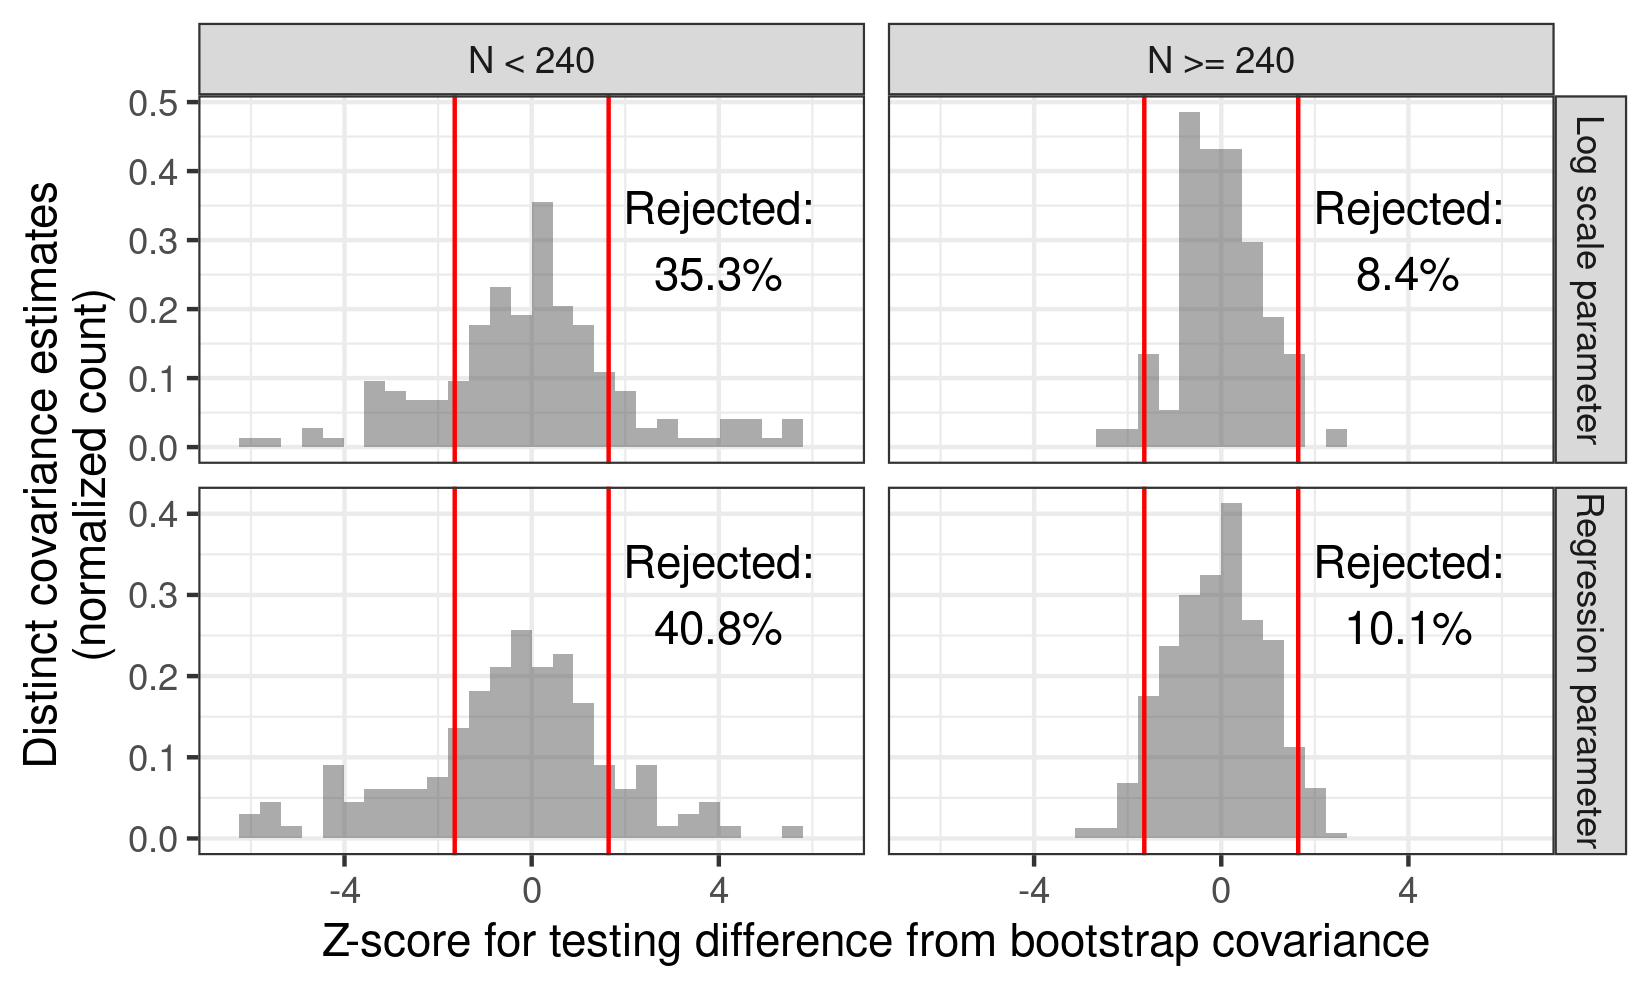
\includegraphics[width=0.98\linewidth,height=0.588\linewidth]{figure/relerr_graph-1} 

}

\caption[The distribution of the z-statistics $\zdiff$]{The distribution of the z-statistics $\zdiff$.  Red lines indicate the boundaries of a two-sided normal test for significance with level $0.1$, and ``Rejected'' gives the percentage of covariances in both sides of the rejection region.  The ``Log scale parameter'' panel includes all variances or covariances that involve at least one log scale parameter.}\label{fig:relerr_graph}
\end{figure}

\end{knitrout}
}


\def\ARMGraphDiff{
%

\begin{knitrout}
\definecolor{shadecolor}{rgb}{0.969, 0.969, 0.969}\color{fgcolor}\begin{figure}[!h]

{\centering 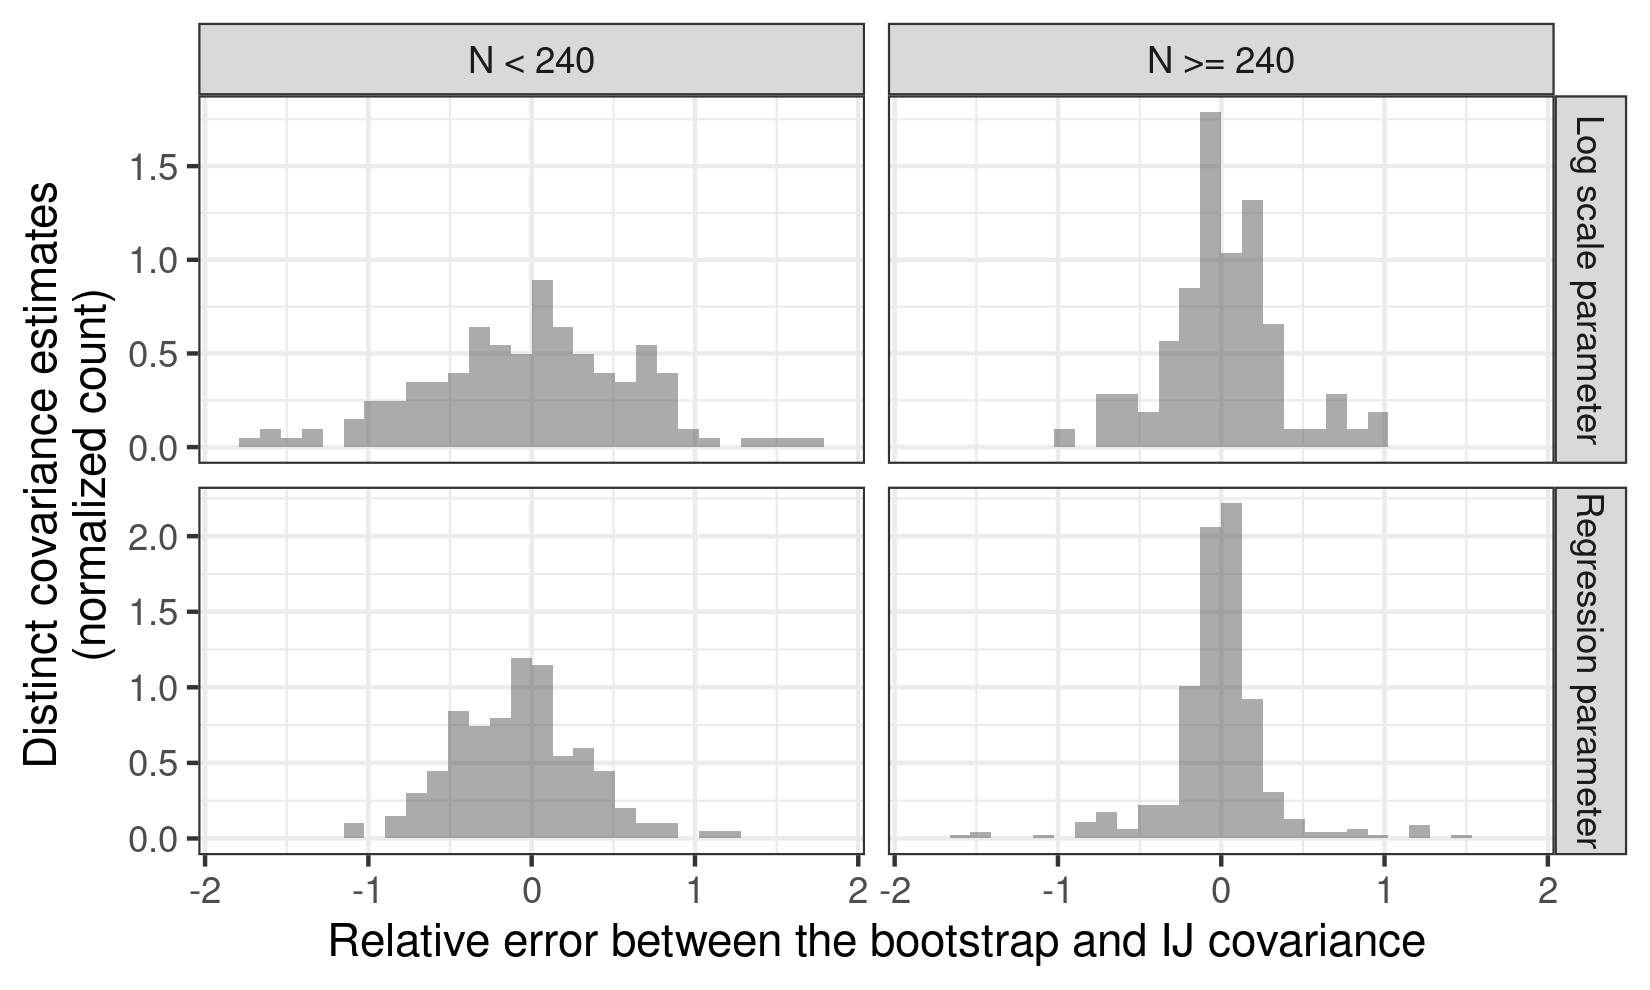
\includegraphics[width=0.98\linewidth,height=0.588\linewidth]{figure/normerr_graph-1} 

}

\caption[The distribution of the relative errors $\normdiffij$]{The distribution of the relative errors $\normdiffij$. The ``Log scale parameter'' panel includes all variances or covariances that involve at least one log scale parameter.}\label{fig:normerr_graph}
\end{figure}

\end{knitrout}
}



\def\ARMGraphPostDiff{
%

\begin{knitrout}
\definecolor{shadecolor}{rgb}{0.969, 0.969, 0.969}\color{fgcolor}\begin{figure}[!h]

{\centering 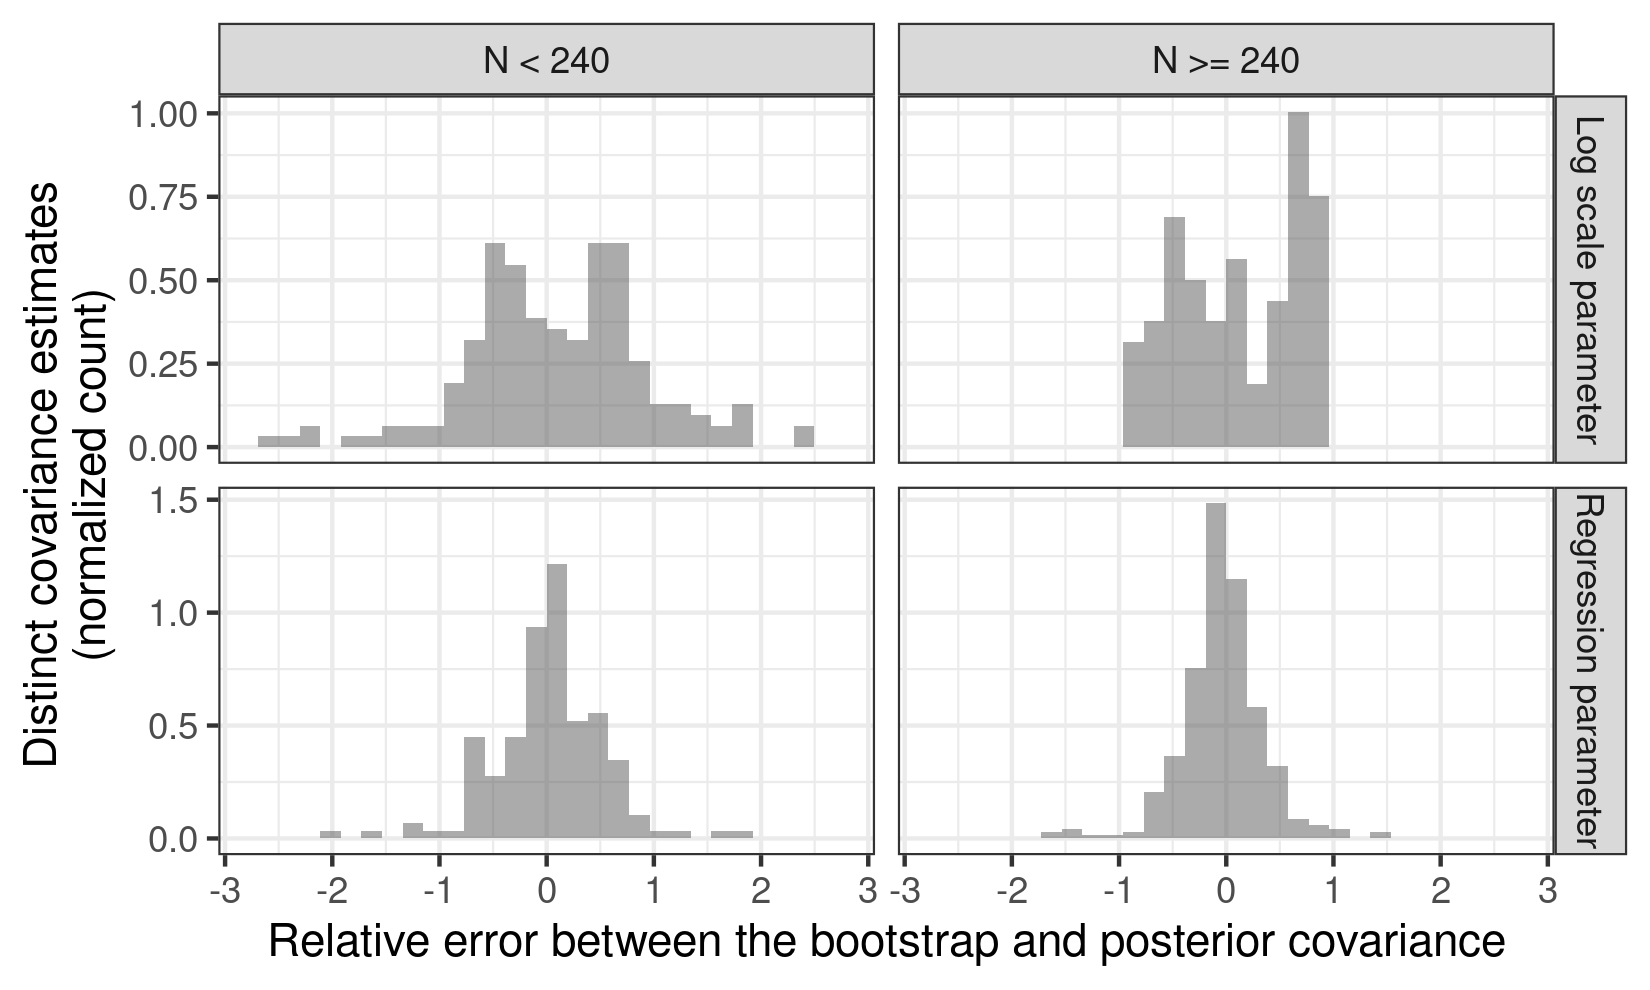
\includegraphics[width=0.98\linewidth,height=0.588\linewidth]{figure/normerr_post_graph-1} 

}

\caption[The distribution of the relative errors $\normdiffbayes$]{The distribution of the relative errors $\normdiffbayes$. The ``Log scale parameter'' panel includes all variances or covariances that involve at least one log scale parameter.}\label{fig:normerr_post_graph}
\end{figure}

\end{knitrout}
}



%%%%%%%%%%%%%%%%%%%%%%%%%%%%%%%%%%%%%%%%%%%%%%%%%%%%%%%%%%%%%%%%%%%%%%%%%
%%%%%%%%%%%%%%%%%%%%%%%%%%%%%%%%%%%%%%%%%%%%%%%%%%%%%%%%%%%%%%%%%%%%%%%%%
%%%%%%%%%%%%%%%%%%%%%%%%%%%%%%%%%%%%%%%%%%%%%%%%%%%%%%%%%%%%%%%%%%%%%%%%%

\def\SingularResultsGraph{

\begin{knitrout}
\definecolor{shadecolor}{rgb}{0.969, 0.969, 0.969}\color{fgcolor}\begin{figure}[!h]

{\centering 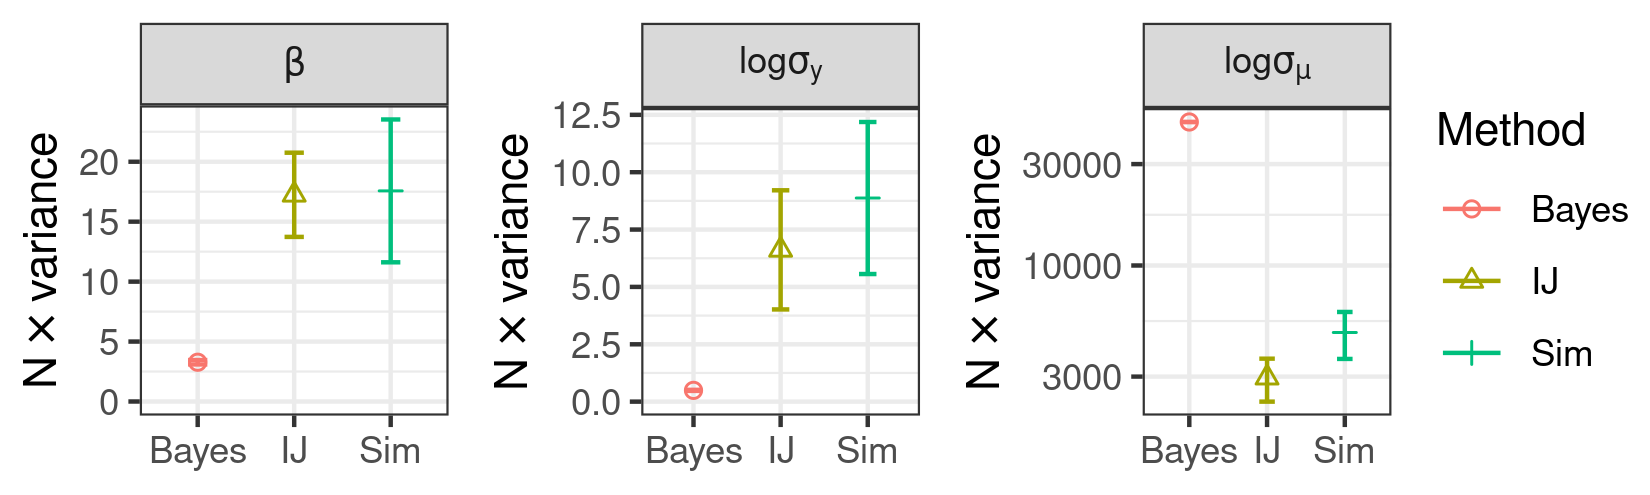
\includegraphics[width=0.98\linewidth,height=0.294\linewidth]{figure/simple_sim_result-1} 

}

\caption[The simulation, IJ, and Bayesian variance estimates, each scaled by $N$]{The simulation, IJ, and Bayesian variance estimates, each scaled by $N$. The right panel uses a log scale.  Error bars show two standard errors.  For the IJ and Bayesian estimates, these include both MCMC error and frequentist sampling error; for the simulation, they reflect the finite number of simulated datasets.  No error bar is shown for the Bayesian posterior variance of $\log \sigma_\mu$.}\label{fig:simple_sim_result}
\end{figure}

\end{knitrout}
%
}



%%%%%%%%%%%%%%%%%%%%%%%%%%%%%%%%%%%%%%%%%%%%%%%%%%%%%%%%%%%%
%%%%%%%%%%%%%%%%%%%%%%%%%%%%%%%%%%%%%%%%%%%%%%%%%%%%%%%%%%%%%%%%%%%%%%%%%
%%%%%%%%%%%%%%%%%%%%%%%%%%%%%%%%%%%%%%%%%%%%%%%%%%%%%%%%%%%%%%%%%%%%%%%%%
%
% <<sim_ar_vars>>=
% sim_ar <- 1.
% sim_img_over_legend <- 2
% sim_r_width <- 2.7
% @

\newcommand{\MRPGraph}{

\begin{knitrout}
\definecolor{shadecolor}{rgb}{0.969, 0.969, 0.969}\color{fgcolor}\begin{figure}[!h]

{\centering 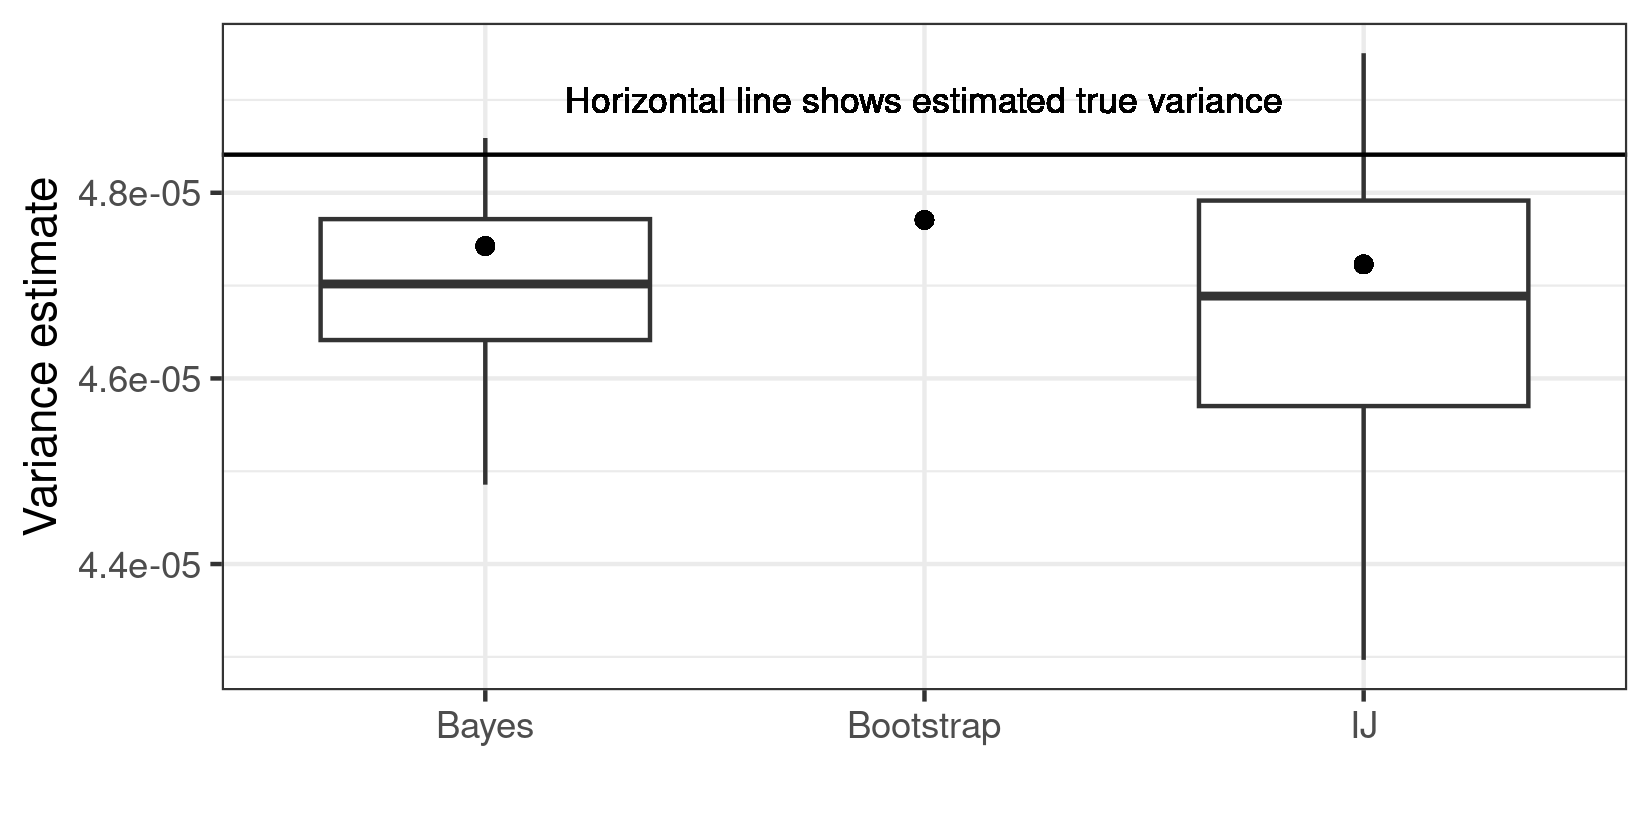
\includegraphics[width=0.98\linewidth,height=0.490\linewidth]{figure/mrp_graph-1} 

}

\caption[Covariance estimates for the MrP model]{Covariance estimates for the MrP model. The dots are the estimates computed on the single dataset chosen as the basis for bootstrapping. The boxplots show the spread of the IJ and posterior covariance across simulations, which includes both frequentist and MCMC variability. The horizontal line shows the true sampling variance as estimated by simulation.}\label{fig:mrp_graph}
\end{figure}

\end{knitrout}
}


\newcommand{\MRPMAPGraph}{

\begin{knitrout}
\definecolor{shadecolor}{rgb}{0.969, 0.969, 0.969}\color{fgcolor}\begin{figure}[!h]

{\centering 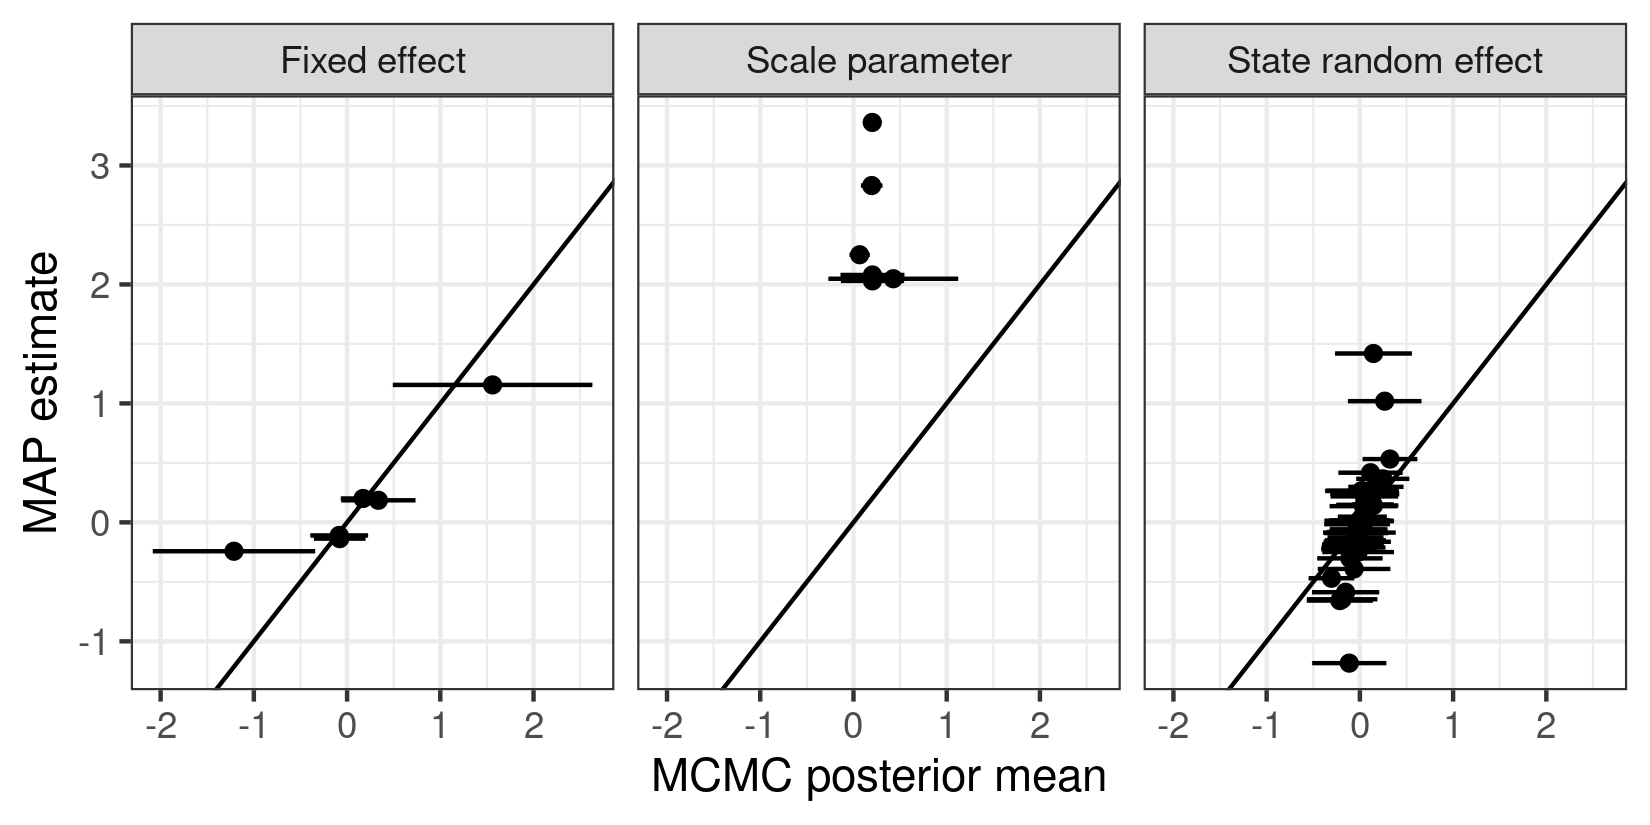
\includegraphics[width=0.98\linewidth,height=0.490\linewidth]{figure/mrp_map_graph-1} 

}

\caption[MAP versus MCMC for the MrP model]{MAP versus MCMC for the MrP model}\label{fig:mrp_map_graph}
\end{figure}

\end{knitrout}
}




\newcommand{\MRPLMERGraph}{

\begin{knitrout}
\definecolor{shadecolor}{rgb}{0.969, 0.969, 0.969}\color{fgcolor}\begin{figure}[!h]

{\centering 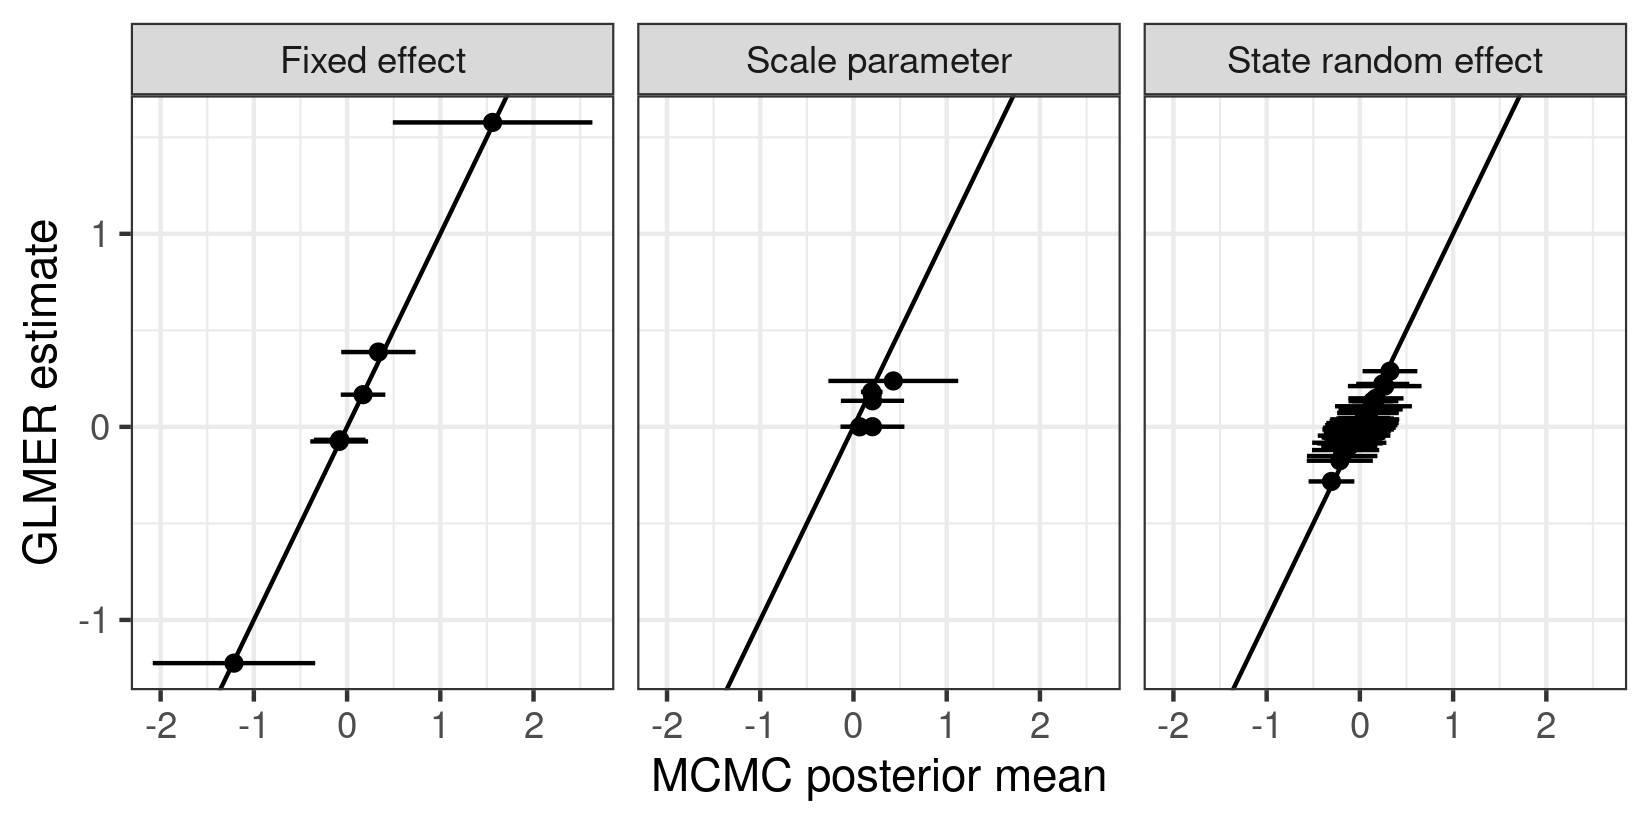
\includegraphics[width=0.98\linewidth,height=0.490\linewidth]{figure/mrp_lmer_graph-1} 

}

\caption[GLMER versus MCMC for the MrP model]{GLMER versus MCMC for the MrP model}\label{fig:mrp_lmer_graph}
\end{figure}

\end{knitrout}
}


\newcommand{\MRPLMERSdGraph}{

\begin{knitrout}
\definecolor{shadecolor}{rgb}{0.969, 0.969, 0.969}\color{fgcolor}\begin{figure}[!h]

{\centering 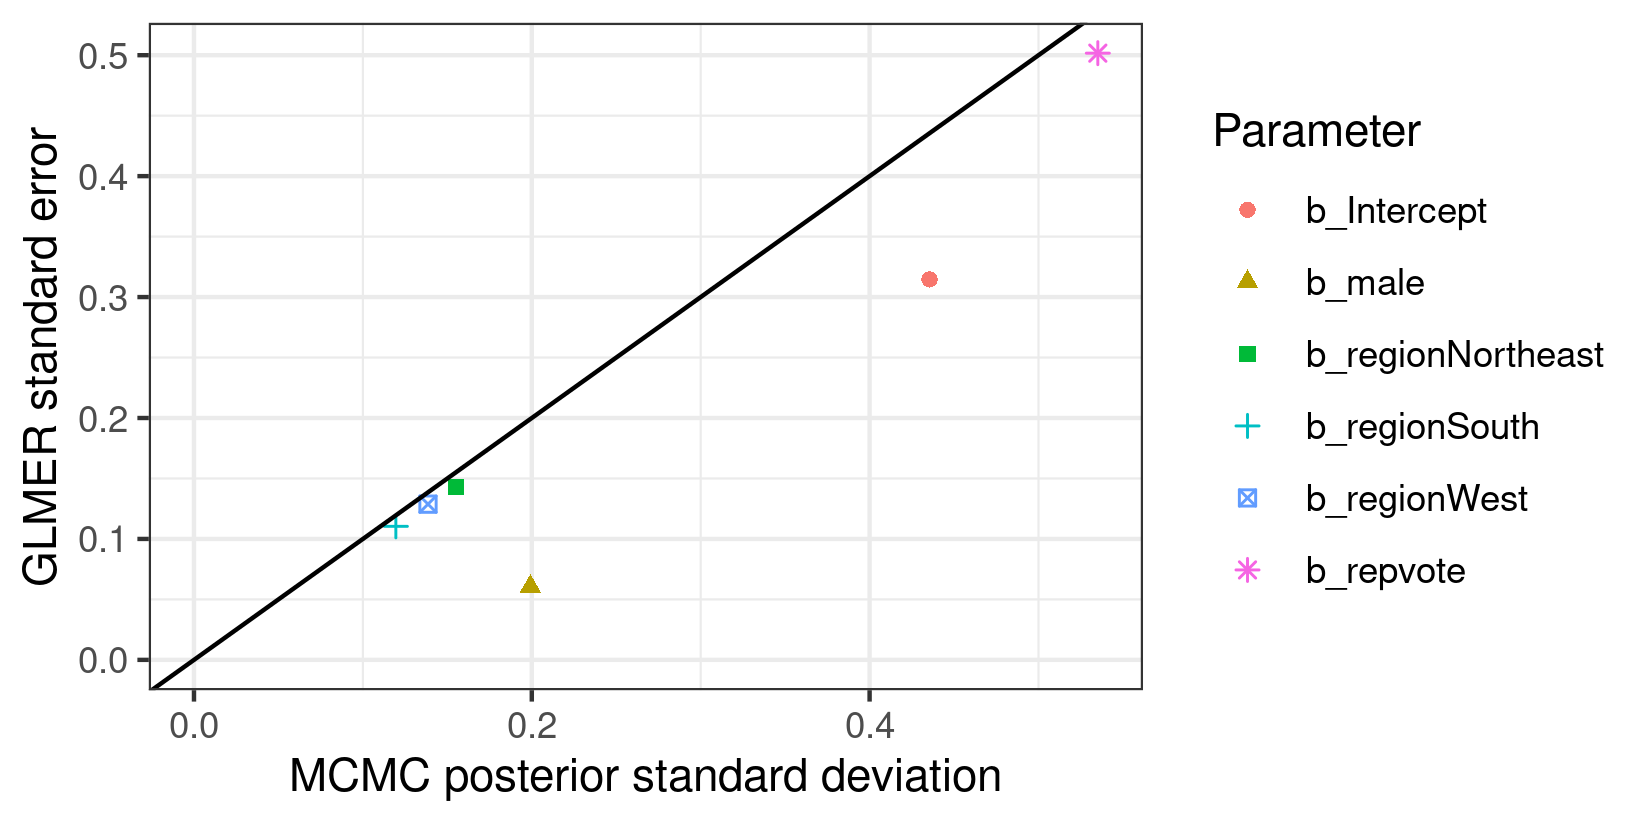
\includegraphics[width=0.98\linewidth,height=0.490\linewidth]{figure/mrp_lmer_sd_graph-1} 

}

\caption[GLMER versus MCMC standard errors for the MrP model]{GLMER versus MCMC standard errors for the MrP model}\label{fig:mrp_lmer_sd_graph}
\end{figure}

\end{knitrout}
}



% \usepackage{lineno}
% \linenumbers



\externaldocument{main}

\begin{document}

\section*{The Bayesian Infinitesimal Jackknife for Variance: Supplemental information and proofs}

\begin{center}
    Ryan Giordano (\texttt{rgiordano@berkeley.edu})
    and\\
    Tamara Broderick (\texttt{tbroderick@mit.edu})
\end{center}

% Prefix the supplement's numbers with "S" so that cross-references between
% the separately compiled main paper and supplement (via xr) are unambiguous.
\renewcommand{\thefigure}{S\arabic{figure}}
\renewcommand{\thetable}{S\arabic{table}}
\renewcommand{\theequation}{S\arabic{equation}}
\renewcommand{\thealgorithm}{S\arabic{algorithm}}
\renewcommand{\theassu}{S\arabic{assu}}
\renewcommand{\thedefn}{S\arabic{defn}}
\renewcommand{\thelem}{S\arabic{lem}}
\renewcommand{\theex}{S\arabic{ex}}
\renewcommand{\thethm}{S\arabic{thm}}
\renewcommand{\theprop}{S\arabic{prop}}
\renewcommand{\thecor}{S\arabic{cor}}
\renewcommand{\thecond}{S\arabic{cond}}
\renewcommand{\theconj}{S\arabic{conj}}




%%%%%%%%%%%%%%%%%%%%%%%%%%%%%%%%%%%%%%%%%%%%%%%%%%%
%%%%%%%%%%%%%%%%%%%%%%%%%%%%%%%%%%%%%%%%%%%%%%%%%%%
% Appendices
%%%%%%%%%%%%%%%%%%%%%%%%%%%%%%%%%%%%%%%%%%%%%%%%%%%
%%%%%%%%%%%%%%%%%%%%%%%%%%%%%%%%%%%%%%%%%%%%%%%%%%%


\appendix

\section{A simple closed-form example}
\applabel{normal_example}
\def\thetagen{\theta_{\mathrm{True}}}
\def\xbar{\tilde{\x}}

In this section, we illustrate verification of our assumptions and the
consistency of the IJ covariance with a simple closed form example, that of
inferring a univariate normal mean with a misspecified variance. More elaborate
examples can be found in \appref{simple_examples_appendix}, including a Poisson
model in the presence of overdispersed data and multilinear regression in the
presence of heteroskedasticity.

For some fixed $\thetagen \in \rdom{}$ and $\sigma^2 \ne 1$, let us
consider the following data generating process and model:
%
\begin{align*}
%
\textrm{Data generating process:}\quad&&
x_n &\iid \normdist(\cdot | \thetagen, \sigma^2) \\
\textrm{Model:}\quad&&
x_n \vert \theta &\iid \normdist(\cdot | \theta, 1) &
\theta &\sim \normdist(\cdot | 0, 1).
%
\end{align*}
%
We will take $\theta$ to be our quantity of interest, so $\g(\theta) = \theta$.
Since $\sigma^2 \ne 1$ the model is misspecified, and so we expect the scaled posterior
variance $N \cov{\post}{\theta}$ to differ from $\gcovtrue$, even asymptotically.

For this simple model, the posterior is available in closed form:
%
\begin{align*}
    \post = \normdist\left( \theta \vert \xbar, (N + 1)^{-1} \right)
    \quad\textrm{where}\quad
    \xbar :={} \frac{1}{N+1} \sumn \x_n.
\end{align*}
%
From this, we can see that $\thetatrue = \lim_{N \rightarrow \infty}
\expect{\post}{\theta} = \thetagen$. It happens in this simple example that
$\thetatrue$ is ``consistent'' for the true mean $\expect{\fdist(\xn)}{\xn}$,
though in general this need not be the case.  For example, the model's trivial
``estimate'' of $\var{\fdist(\xn)}{\xn}$ is $1$, which is never equal to the
true value of $\sigma^2$.

One can readily verify that \assuref{bayes_clt,bclt_okay} are satisfied for this
model and this particular value of $\thetatrue$. Arguably the most challenging
condition is the final part of \assuref{bayes_clt} \itemref{strict_opt}, which
one can show via strong concavity of the log likelihood, together with
convergence of $\frac{1}{N} \sumn \ellgrad{1}(\x_n \vert \thetatrue) \plim 0$ by
the ordinary law of large numbers.  Using special structure of a particular
problem (like strong concavity) to establish a condition like
\assuref{bayes_clt} \itemref{strict_opt} is common in the literature --- see,
for example, textbook proofs of the consistency of M-estimators on unbounded
domains (e.g.~Theorem 9.11 of \citet{keener:2010:theoretical} or Chapter 6.2 of
\citep{huber:2011:robust}).

We begin by establishing \corref{bayes_expectation_dist} and identifying our target,
$\gcovtrue$. By the ordinary CLT applied to our closed-form expression for
$\expect{\post}{\theta}$, we have that
$$
\sqrt{N}\left(\expect{\post}{\theta} - \thetatrue\right) \dlim
\normdist\left(\cdot \vert 0, \sigma^2 \right),
$$
from which we see that $\gcovtrue = \sigma^2$.  It happens, in this case, that
the variance of the limiting distribution is also the limit of the variance,
since
$$
N \var{\xfdist}{\expect{\post}{\theta}} =
    \frac{N^2}{(N+1)^2}\sigma^2 \rightarrow \sigma^2 = \gcovtrue.
$$
The asymptotic equivalence between the variance of the limit and the limit of
the variance occurs in this case because the rescaled squared errors
$N \left(\expect{\post}{\theta} - \thetatrue\right)^2$ are uniformly
integrable in $N$ (Theorem 10.3.6 of \citet{dudley:2018:realanalysis}).
%
We emphasize, however, that our theorems do
not assume uniform integrability, and we aim to estimate the variance of the
limiting normal distribution, not the limiting value of the variance, as
discussed in the text surrounding \eqref{gtrue}.

To complete \corref{bayes_expectation_dist}, we need to show that the expression
for $\gcovtrue$ is correct. In this case, $\ggrad{1}(\theta) = 1$, and the
remaining quantities are (up to constants not depending on
$\theta$):
\begin{align}
%
\log \pi(\theta) ={}& -\frac{1}{2}\theta^2 + \textrm{Constant}
\quad\textrm{and}\quad
% \nonumber\\
\likhat(\theta) ={}
    -\frac{1}{2N} \sumn \left(x_n^2 - 2x_n \theta + \theta^2\right)
    -\frac{1}{2N} \theta^2 + \textrm{Constant} \Rightarrow \nonumber \\
\thetahat ={}& \xbar
\quad\textrm{,}\quad
\ellgrad{1}(\x_n \vert \theta) ={} x_n - \theta
\quad\textrm{and}\quad
\likhatk{2}(\theta) ={} -\frac{N+1}{N} \Rightarrow \nonumber \\
\scorecovhat ={}& \meann \left(x_n - \xbar\right)^2
\quad\textrm{,}\quad
\infohat ={} \frac{N+1}{N}
\quad\textrm{and}\quad
\gcovhat ={} \infohat^{-1} \scorecovhat \infohat^{-1} =
    \frac{N^2}{(N + 1)^2} \scorecovhat.
\eqlabel{normal_gcovhat}
%
\end{align}
%
It is readily verified that $\gcovhat \plim \sigma^2 = \gcovtrue$,
so we have verified the conclusion of \corref{bayes_expectation_dist}.

Finally, we manually verify \thmref{ij_consistent}. The influence score is given by:
%
\begin{align*}
%
\infl_n ={}& N \cov{\post}{
    \theta, -\frac{1}{2} \left(\x_n^2 - 2\x_n \theta + \theta^2 \right)} \\
={}&
 -\frac{1}{2}  N \cov{\post}{\theta, 1} \x_n^2 +
 N \cov{\post}{\theta, \theta} \x_n
 -\frac{1}{2} N  \cov{\post}{\theta, \theta^2}
={} \frac{N}{N+1} \x_n + \textrm{Constant},
%
\end{align*}
%
where the constant in the final line is the same for all $\x_n$.  Since the IJ covariance
depends only on the difference $\infl_n - \bar{\infl}$, quantities that are the
same for each $n$ can be neglected in the IJ covariance computation. Therefore
the IJ covariance estimate is given by
%
\begin{align*}
%
\gcovij ={}& \meann \left(\infl_n - \bar{\infl} \right)^2
={} \frac{N^2}{(N + 1)^2} \meann \left(\x_n - \bar{\x}\right)^2
\plim \sigma^2 = \gcovtrue,
\quad\textrm{where}\quad
\bar{\x} := \meann \x_n.
%
\end{align*}
%
Since $\scorecovhat = \meann \left(\x_n - \bar{\x}\right)^2 + \left(\bar{\x} -
\xbar\right)^2$ and $\bar{\x} - \xbar = \bar{\x} / (N + 1) = O_p(N^{-1})$,
$\gcovij$ differs from the $\gcovhat$ given in \eqref{normal_gcovhat} only by
a term of order $O_p(N^{-2})$.  So, like $\gcovhat$, $\gcovij$ is a
consistent estimator of the asymptotic variance $\gcovtrue$.


%%%%%%%%%%%%%%%%%%%%%%%%%%%%%%%%%%%%%%

\section{Notation key}
For ease of reference, we provide here a table of key quantities
defined and used through the course of our proofs.

\begin{table}[!h]
\begin{tabular}{|c|c|c|}
\hline
Symbol & Description & Definition \\
\hline
$\infl_n$ & Influence score of the $n$--th observation & \eqref{ij_terms}\\
\hline
$\indexset$ & A set of sets of data indices & \defref{index_sets} \\
\hline
$\xvec_s$ & The observations corresponding to $s \in \indexset$ & \defref{index_sets} \\
\hline
$\phi(\theta, \xvec_s)$ &
    A function of interest depending on $\theta$ and a set of datapoints &
    \defref{bclt_okay_index} \\
\hline
$\thetaball{\delta}$ & A $\delta$-ball around $\thetatrue$ & \assuref{bayes_clt} \\
\hline
$\tresid{k}{\phi, \thetahat, \theta}$ & The $k$--th order Taylor series residual term for $\phi$ &
    \defref{taylor_residual} \\
\hline
$\normhatarg{\tau}$ & Gaussian density with covariance $\infohat^{-1}$  & \defref{gaussian_defs} \\
\hline
$\normresid{\lambda}{S}(\tau)$ &
    Isotropic Gaussian density with precision $\lambda$ truncated to set $S$ &
    \defref{gaussian_defs} \\
\hline
$\normalizer$ & Normalizing constant for $\normhatarg{\tau}$& \defref{gaussian_defs} \\
\hline
$\infoev,\infoevhat$ & Minimum eigenvalues of $\info$, $\infohat$ & \defref{loglik_details_def} \\
\hline
$\tau$ & Centered and scaled parameter $\sqrt{N}(\theta - \thetahat)$ & \eqref{tau_defn} \\
\hline
$R_1,R_2,R_3$ & Inner, middle, and outer regions of integration & \defref{region_division} \\
\hline
$\delta_1$ & Scale of boundary between $R_1$ and $R_2$ & \defref{region_division} \\
\hline
$\delta_2$ & Scale of boundary between $R_2$ and $R_3$ & \defref{region_division} \\
\hline
$I(\phi)$ & The integration functional of $\phi$ & \eqref{integral_funcational} \\
\hline
$I_k(\phi)$ & Integration functional restricted to region $R_k$ &
    \eqref{region_integration_functional} \\
\hline
$\regevent$ & The event that the problem is ``regular'' & \lemref{regular_event} \\
\hline
$\epsilon_U$ & Arbitrarily small accuracy parameter for the regular event & \lemref{regular_event} \\
\hline
$\epsilon_L$ & Log likelihood lower bound in regular event & \lemref{regular_event} \\
\hline
$\resid{\phi}(\xvec_s)$ & The BCLT residual for $\expect{\post}{\phi(\theta, \xvec_s)}$ &
    \defref{bclt_resid} \\
\hline
$\resid{k}(\xvec_s)$ & The $k$--th component of the BCLT residual & \defref{bclt_resid} \\
\hline
\end{tabular}
\caption{Notation key}\label{tab:notation_key}
\end{table}


\section{Setup and Preliminaries}

\subsection{Derivative arrays}


Throughout our proofs, we will be forming and manipulating higher-order
Taylor expansions of functions of $\theta$.  The arrays of derivatives
in these expressions will always be summed against a direction, typically
$\tau = \sqrt{N}(\theta - \thetahat)$.  In order to avoid cumbersome
summation notation for all such terms, we will implicitly sum derivative arrays
against $\tau$ or $\theta$.  For example, for
a function $\psi(\theta, \x_n) \in \rdom{D_\psi}$, we will write
%
\begin{align*}
\psigrad{3}(\thetahat, \x_n)\tau^3 =
\sum_{a=1}^D \sum_{b=1}^D \sum_{c=1}^D
    \fracat{\partial^3 \psi(\theta, \x_n)}
           {\partial\theta_{a} \partial\theta_{b} \partial\theta_{c}}
           {\thetahat} \tau_{a} \tau_{b} \tau_{c}.
\end{align*}
%
Occasionally we will need to sum several derivative arrays against $\tau$,
particularly in \secref{region_r1}.  Since the directions $\tau$ will always be
the same, we will combine the $\tau$ in such expressions with no ambiguity. For
example, for the term involving $\likhatk{3}(\thetahat)$ in the statement of
\thmref{bayes_clt_main}, we will write
%
\begin{align*}
%
\psigrad{1}(\thetahat, \x) \likhatk{3}(\thetahat) \tau^4 =
\sum_{a=1}^{D} \sum_{b=1}^{D} \sum_{c=1}^{D} \sum_{d=1}^{D}
    \psigrad{1:a}(\thetahat, \x) \likhatk{3:b,c,d}(\thetahat)
    \tau_a \tau_b \tau_c \tau_d.
%
\end{align*}
%

When necessary, higher
derivatives will be indexed in the parentheses.  For example,
$\psigrad{2:i,j}(\theta, \x_n)$ will denote the length--$D_\psi$ vector
%
\begin{align*}
%
\fracat{\partial^2 \psi(\theta, \x_n)}
    {\partial\theta_i \partial\theta_j}{\theta}.
%
\end{align*}
%
%\end{defn}

We denote by $\ind{A}$ the indicator function taking value $1$ when the
event $A$ occurs and $0$ otherwise.

% Order notation
We will use order notation to describe the behavior of quantities as $N
\rightarrow \infty$.  For example, we will use $z = O(\phi(N))$ to mean there
exists an $N^*$ and an $A > 0$ such that $N > N^* \Rightarrow z < A \phi(N)$. In
our notation, $A$ and $N^*$ in this definition will never depend on the data,
$\xvec$, though they may depend on unobserved population quantities.
%
Dependence on the data $\xvec$ in order notation will always be represented with
$O_p$ notation.  For example, $z = O_p(\phi(N))$ will mean that there exists an
$A > 0$ such that for any $\epsilon > 0$, there is a corresponding $N^*$ and
such that
%
\begin{align*}
%
N > N^* \quad\Rightarrow\quad
    \expect{\xfdist}{\ind{z < A \phi(N)}} > 1 - \epsilon.
%
\end{align*}
%
Here, $A$ does not depend on $\epsilon$.  The meaning is that the event $z =
O(\phi(N))$ occurs with arbitrarily high probability as $N$ goes to infinity.
The notation $\tilde{O}$ and $\tilde{O}_p$ will have the same meaning as $O$ and
$O_p$ notation respectively, but with factors of $\log N$ possibly ignored.


\subsection{General index sets}\seclabel{index_sets}

%%%%%%%%%%%%%%%%%%%%%%%%%%%%%%%%%%%%%%%%%%%%%%%%%%%%%
% Index sets

To succinctly state our theorems for double sums, it will be convenient to
introduce a more general index notation.

\begin{defn}\deflabel{index_sets}
    %
    Let $\indexset$ denote a set of sets of data indices, where each member $s \in
    \indexset$ has the same cardinality, and for $s \in \indexset$, let $\xvec_s$
    denote the set of corresponding datapoints.  We write $\phi(\xvec_s)$ for a
    function that depends on $|s|$ datapoints.  For example, if $\indexset = \{1,
    \ldots, N \} =: [N]$, then $\xvec_s = \x_s$, and $\means \phi(\xvec_s) = \meann
    \phi(\x_n)$.  Similarly, if $\indexset = [N] \times [N]$, then $\xvec_s =
    (\x_{s_1}, \x_{s_2})$, and $\means \phi(\xvec_s) = \frac{1}{N^2} \sum_{n=1}^N
    \sum_{m=1}^N \phi(\x_n, \x_m)$.
    %
\end{defn}

We now state a generalization of \defref{bclt_okay} that applies to 
generic index sets as defined in \defref{index_sets}.

\begin{defn}\deflabel{bclt_okay_index}
%
For an index set $\indexset$, a data-dependent function
$\phi(\theta, \xvec_s)$ is $K$-th order BCLT-okay if
%
\begin{enumerate}
%
\item\itemlabel{bclt_okay_as_index}
    $\theta \mapsto \phi(\theta, \xvec_s)$
    is $K$ times continuously differentiable $\fdist$--almost surely.
%
\item\itemlabel{prior_op1_index}
    $\means \expect{\prior(\theta)}{\norm{\phi(\theta, \xvec_s)}^2_2} = O_p(1)$.
%
\item\itemlabel{grad_op1_index}
For some $\delta > 0$, and for each $k = 0, \ldots, K$,
$\sup_{\theta \in \thetaball{\delta}}
    \means \norm{\phigrad{k}(\theta, \xvec_s)}^2_2 = O_p(1)$.
%
\end{enumerate}
%
\end{defn}


Note that a function is BCLT-okay according to \defref{bclt_okay} precisely if
it is BCLT-okay according to \defref{bclt_okay_index} with index set $\indexset
= [N]$.  Although $\indexset = [N]$ and $\indexset = [N]\times[N]$ will be the
only examples of $\indexset$ we will use in the present paper, we believe it is
clearer to keep the notation general.   

In particular, \thmref{bayes_clt_main} is stated in terms of $\indexset = [N]$,
but we will prove that it holds for generic index sets of the form
\defref{bclt_okay_index}.  Formally, we will prove \thmref{bayes_clt_main} under
the following \assuref{core_bclt_assu}, noting that \assuref{core_bclt_assu} is
assumed by \thmref{bayes_clt_main} for $\indexset = [N]$.

\begin{assu}\assulabel{core_bclt_assu}
%
Assume that $\phi(\theta, \xvec_s)$ is third-order BCLT-okay
according to \defref{bclt_okay_index}, and that \assuref{bayes_clt} holds.
%
\end{assu}


\subsection{Taylor series expansions and their asymptotics}\applabel{loglik_asymptotics}
The proofs below repeatedly rely on two key ideas: Taylor series
expansions, and uniform asymptotic control on the terms that arise.
In this section, we introduce these ideas and prove two key
lemmas.  The first, \lemref{taylor_residual}, gives the form
of a Taylor series expansion.  The second, \lemref{ulln},
controls the asymptotic behavior of the log likelihood
and its derivatives in a neighborhood of $\thetatrue$.


%%%%%%%%%%%%%%%%%%%%%%%%%%%%%%%%%%%%%%%%%
%%%%%%%%%%%%%%%%%%%%%%%%%%%%%%%%%%%%%%%%%
%%%%%%%%%%%%%%%%%%%%%%%%%%%%%%%%%%%%%%%%%


\subsubsection{Taylor series expansions}

Our analysis is based strongly on Taylor series expansions.
We will use the following two minor variants of standard analysis tools.
The first is a multivariate version of the integral form of the Taylor series
residual for a vector-valued function.

\begin{defn}\deflabel{taylor_residual}
%
For a $k$-times differentiable function $\phi(\theta)$, a fixed $\thetahat$,
and $\theta$, define the residual functional
%
\begin{align*}
%
\tresid{k}{\phi, \thetahat, \theta} :=
    \frac{1}{(k-1)!} \int_0^1 (1 - t)^{k-1}
        \phigrad{k}(\thetahat + t (\theta - \thetahat)) dt.
%
\end{align*}
%
\end{defn}
%
The residual $\tresid{k}{\phi, \thetahat, \theta}$ is an array of the same
dimension as the $k$-th order derivative, $\phigrad{k}(\theta)$.  Observe that,
for any norm $\norm{\cdot}$,
%
\begin{align*}
    %
    \norm{\tresid{k}{\phi, \thetahat, \theta}} \le
        \frac{1}{(k-1)!} \sup_{\thetatil: \norm{\thetatil - \thetahat}_\infty \le
                                          \norm{\theta - \thetahat}_\infty}
                            \norm{\phigrad{k}(\thetatil)}.
    %
\end{align*}
%
\begin{lem}\lemlabel{taylor_residual}
%
A $K$-times continuously differentiable function $\phi(\theta)$ has Taylor
series residual
%
\begin{align*}
\phi(\theta) =
    \sum_{k=0}^{K-1} \frac{1}{k!} \phigrad{k}(\thetahat) (\theta - \thetahat)^k +
    \tresid{K}{\phi, \thetahat, \theta} (\theta - \thetahat)^K.
\end{align*}
%
\begin{proof}
%
Let $\phi_d(\theta)$ denote the $d$-th component of the vector $\phi(\theta)$
(contrast this notation with the $d$-th order derivative
$\phigrad{d}(\theta)$). Consider the scalar to scalar map $t \mapsto
\phi_d(\thetahat + t (\theta - \thetahat))$. Taking the integral remainder form
of the $K - 1$-th order Taylor series expansion of this scalar map
\citep[Appendix B.2]{dudley:2018:analysis} and stacking the result into a vector
gives the desired result.
%
\end{proof}
%
\end{lem}



%%%%%%%%%%%%%%%%%%%%%%%%%%%%%%%%%%%%%%%%%
%%%%%%%%%%%%%%%%%%%%%%%%%%%%%%%%%%%%%%%%%
%%%%%%%%%%%%%%%%%%%%%%%%%%%%%%%%%%%%%%%%%

\subsubsection{Log likelihood asymptotics}

To use \lemref{taylor_residual} to study $\likhat(\theta)$, we will need to
expand \defref{loglik_def} with the following quantities.

%%%%%%%%%%%%%%%%%%%%%%%%%%%%%%%%%%%%%%%%
%%%%%%%%%%%%%%%%%%%%%%%%%%%%%%%%%%%%%%%%
\begin{defn}\deflabel{loglik_details_def}
\begin{align*}
%
\likhatk{k}(\theta) :={}&
   \frac{1}{N} \sumn \ellgrad{k}(\x_n \vert \theta) +
    %\frac{1}{N} \frac{\prior_{(k)}(\theta)}{\prior(\theta)} % NOT CORRECT
    \frac{1}{N} \logpriorgrad{k}(\theta)
&
\likk{k}(\theta) :={}& \int \ellgrad{k}(\xn \vert \theta) d\fdist(\xn)
\\
\infoev :={}& \textrm{The minimum eigenvalue of }\info &
\infoevhat :={}& \textrm{The minimum eigenvalue of }\infohat
%
\end{align*}
%
Note that, following our convention, $\likhatk{k}(\theta)$ is the $k$--th
partial derivative of $\likhat(\theta)$ with respect to $\theta$.

The term $\likk{k}(\theta)$ is a potential abuse of notation, since it is only
the partial derivative of $\lik(\theta)$ under the assumption that we can
interchange integration and differentiation.  Though we will in fact be assuming
sufficient conditions for this interchange (\assuref{bayes_clt}
\itemref{loglik_ulln}), our proofs will simply use the above definition of
$\likk{k}(\theta)$ directly.
\end{defn}
%
Using \lemref{taylor_residual}, we can then form a Taylor series expansion
around $\thetahat$, an expression that we will analyze carefully in
\appref{bayes_clt_proof}:
%
\begin{align}
\likhat(\theta) ={}&
    \likhat(\thetahat) +
    \likhatk{1}(\thetahat)(\theta - \thetahat) +
    \frac{1}{2}\likhatk{2}(\thetahat)(\theta - \thetahat)^2 +
\nonumber
\\&
    \frac{1}{6}\likhatk{3}(\thetahat)(\theta - \thetahat)^3 +
    \tresid{4}{\likhat, \thetahat, \theta} (\theta - \thetahat)^4.
    \eqlabel{loglik_series_example}
\end{align}
%

We now turn to the task of controlling the kinds of terms that arise in
\eqref{loglik_series_example}. One of our key tools in the proof of
\lemref{ulln} will be \emph{uniform laws of large numbers} (ULLNs), a concept
which we make concrete in \defref{ulln}. Typically, ULLNs require that the
sample average $\meann \phi(\x_n, \theta)$ converge to
$\expect{\fdist(\xn)}{\phi(\x_n, \theta)}$ uniformly over $\theta$ in some
compact set.
%
%%%%%%%%%%%%%%%%%%%%%%%%%%%%%%%%%%%%%%%%%%%%%
%%%%%%%%%%%%%%%%%%%%%%%%%%%%%%%%%%%%%%%%%%%%%
\begin{defn}\deflabel{ulln}
%
Recall the definition of $\thetaball{\delta}$ from \assuref{bayes_clt}. We say a
``uniform law of large numbers'', or ``ULLN'', holds for a function
$\phi(\theta, \xn)$ if, for some $\delta > 0$,
%
\begin{align*}
%
\sup_{\theta \in \thetaball{\delta}}
\norm{\meann \phi(\theta, \x_n) -
\expect{\fdist(\xn)}{\phi(\theta, \xn)}}_2
\plim 0,
%
\end{align*}
%
where $\expect{\fdist(\xn)}{\phi(\theta, \xn)}$ is finite.
%
\end{defn}
%%%%%%%%%%%%%%%%%%%%%%%%%%%%%%%%%%%%%%%%%%%%%

In general, a ULLN requires that the set of functions $\left\{\theta \mapsto
\phi(\theta, \xvec): \norm{\theta - \thetatrue}_2 < \delta \right\}$ be a
``Glivenko-Cantelli class'' with finite covering number (Chapter 19 of
\citet{van:2000:asymptotic}, \citet{vaart:2013:empiricalprocesses}). A simple
condition for a uniform law of large numbers to hold is that $\phi(\theta, \xn)$
be dominated by an absolutely integrable function of $\xn$ alone in a compact
neighborhood of $\thetatrue$ (Example 19.7 of \citet{van:2000:asymptotic}).

We now state a key lemma controlling the asymptotic behavior of the log
likelihood and its derivatives.

%%%%%%%%%%%%%%%%%%%%%%%%%%%%%%%%%%%%%%%%%%%%%%%%%%%
%%%%%%%%%%%%%%%%%%%%%%%%%%%%%%%%%%%%%%%%%%%%%%%%%%%
%%%%%%%%%%%%%%%%%%%%%%%%%%%%%%%%%%%%%%%%%%%%%%%%%%%

\begin{lem}\lemlabel{ulln}
%
Suppose that there exists $\deltaulln > 0$, $M(\xn)$, and $K \ge 1$ such that
%
\begin{align}
%
\sup_{\theta \in \thetaball{\deltaulln}}
    \norm{\ellgrad{K}(\xn \vert \theta)}_2 \le M(\xn)
\quad\textrm{with}\quad
\expect{\fdist(\xn)}{M(\xn)^2} < \infty.
\eqlabel{bounded_lipschitz}
%
\end{align}
%
Additionally assume that $\pi(\theta)$ is non-zero and $K-1$ times
continuously differentiable in $\thetaball{\deltaulln}$.  Assume also that
%
\begin{align}
    \expect{\fdist(\xn)}{\norm{\ellgrad{k}(\xn \vert \thetatrue)}^2_2} < \infty
    \textrm{ for }k=0,\ldots, K-1.
    \eqlabel{ellgrad_bounded_moments}
\end{align}
%
Then the following results hold.  First, for $k \in \{0, \ldots, K\}$,
%
\begin{align}
\sup_{\theta \in \thetaball{\deltaulln}}
    \meann \norm{\ellgrad{k}(\x_n \vert \theta)}_2^2
     &={} \ordp{1}
% \nonumber\\&\hspace{-3em}
     \eqlabel{means_op1}.
%
\end{align}
%
Then, for $k \in \{0, \ldots, K - 1\}$,
%
\begin{align}
%
\sup_{\theta \in \thetaball{\deltaulln}}
    \norm{\meann \left( \ellgrad{k}(\x_n \vert \theta) -
           \expect{\fdist(\xn)}{\ellgrad{k}(\xn \vert \theta)} \right)
           }_2 &\plim{} 0
         \eqlabel{glivenko_cantelli} \\
%
% \sup_{\theta \in \thetaball{\deltaulln}}
%     \norm{\frac{1}{\sqrt{N}} \sumn \left( \ellgrad{k}(\x_n \vert \theta) -
%            \expect{\fdist(\xn)}{\ellgrad{k}(\xn \vert \theta)}\right)
%            }_2 &={} \ordp{1}
%            \eqlabel{donsker} \\
%
\sup_{\theta \in \thetaball{\deltaulln}}
    \norm{\likhatk{k}(\theta) - \likk{k}(\theta)}_2 &\plim{} 0.
         \eqlabel{ulln}
%
\end{align}
%
%%%%%%%%%%%%%%%%%%%%%%%%%%%%%%%%%%%%%%%%%%
%%%%%%%%%%%%%%%%%%%%%%%%%%%%%%%%%%%%%%%%%%
\begin{proof}
%
First, note that
%
\begin{align*}
%
\sup_{\theta \in \thetaball{\deltaulln}}
    \meann \norm{\ellgrad{K}(\x_n \vert \theta)}_2^2 \le{}&
\meann \sup_{\theta \in \thetaball{\deltaulln}}
    \norm{\ellgrad{K}(\x_n \vert \theta)}_2^2
\quad\textrm{and}\\
\expect{\fdist(\xn)}{
    \sup_{\theta \in \thetaball{\deltaulln}}
        \norm{\ellgrad{K}(\xn \vert \theta)}^2_2
} \le{}& \expect{\fdist(\xn)}{M(\xn)^2} < \infty,
%
\end{align*}
%
so \eqref{means_op1} holds for $k = K$ by the strong law of large numbers.

We now prove the remaining relations inductively. For a scalar--valued,
differentiable function $f(\theta)$, and any two $\theta, \theta'$ in
$\thetaball{\deltaulln}$, we can write
%
\begin{align*}
%
\abs{f(\theta) - f(\theta')} ={}&
\abs{
    \int_0^1 \fracat{\partial f(\theta' + \t (\theta - \theta'))}
                    {\partial \t}{\t} d\t
}
\\={}&
\abs{
    \int_0^1 f_{(1)}(\theta' + \t (\theta - \theta')) (\theta - \theta') d\t
}
\\\le{}&
    \norm{\theta - \theta'}_2
    \sup_{\thetatil \in \thetaball{\deltaulln}}
        \norm{f_{(1)}(\thetatil)}_2.
%
\end{align*}
%
Applying the previous formula componentwise to $\ellgrad{K-1}(\xn \vert
\theta)$, and loosening the right hand side to contain all of
$\norm{\ellgrad{K}(\xn \vert \thetatil)}_2$ rather than only a particular
component, gives
%
\begin{align}
%
\norm{\ellgrad{K-1}(\xn \vert \theta) - \ellgrad{K-1}(\xn \vert \theta')}_\infty \le{}&
    \norm{\theta - \theta'}_2
    \sup_{\thetatil \in \thetaball{\deltaulln}}
        \norm{\ellgrad{K}(\xn \vert \thetatil)}_2
\nonumber \\\le{}&
\norm{\theta - \theta'}_2 M(\xn). \eqlabel{ellgrad_linf_bound}
%
\end{align}
%
It follows that each component of $\ellgrad{K-1}(\xn \vert \theta)$ is
Glivenko-Cantelli, and so \eqref{glivenko_cantelli} holds for
$k = K - 1$, using also \eqref{bounded_lipschitz} and
\eqref{ellgrad_bounded_moments} for square integrability
(see \cite[Example 19.7]{van:2000:asymptotic},
as well as the discussion in \defref{ulln} above).  Further, evaluating
\eqref{ellgrad_linf_bound} at $\theta' = \thetatrue$ and taking the
supremum gives
%
\begin{align*}
\sup_{\theta \in \thetaball{\deltaulln}}
    \norm{\ellgrad{K-1}(\xn \vert \theta)}^2_2
\le{}&
\thetadim^{K-1}
\sup_{\theta \in \thetaball{\deltaulln}}
    \norm{\ellgrad{K-1}(\xn \vert \theta)}_\infty^2
\\\le{}&
2 \thetadim^{K-1}
\sup_{\theta \in \thetaball{\deltaulln}}
    \norm{
        \ellgrad{K-1}(\xn \vert \theta) -
        \ellgrad{K-1}(\xn \vert \thetatrue)}_\infty^2 +
2 \thetadim^{K-1}
 \norm{\ellgrad{K-1}(\xn \vert \thetatrue)}_\infty^2
\\\le{}&
2 \thetadim^{K-1}
\sup_{\theta \in \thetaball{\deltaulln}}
\norm{\theta - \thetatrue}^2_2 M(\xn)^2 +
2 \thetadim^{K-1}
 \norm{\ellgrad{K-1}(\xn \vert \thetatrue)}_2^2
\\\le{}&
2 \deltaulln^2 \thetadim^{K-1} M(\xn)^2 +
2 \thetadim^{K-1} \norm{\ellgrad{K-1}(\xn \vert \thetatrue)}_2^2.
\end{align*}
%
It follows from \eqref{bounded_lipschitz} and \eqref{ellgrad_bounded_moments}
with $k = K - 1$ that
$$
\expect{\fdist(\xn)}{\sup_{\theta \in \thetaball{\deltaulln}}
    \norm{\ellgrad{K-1}(\xn \vert \theta)}^2_2} < \infty,
$$
and so \eqref{means_op1} holds for $k = K - 1$ by applying the LLN
to the envelope function
$\sup_{\theta \in \thetaball{\deltaulln}}
    \norm{\ellgrad{K-1}(\xn \vert \theta)}^2_2$.

Since \eqref{bounded_lipschitz} holds for $k=K-1$ with the envelope
$M_{K-1}(\xn) := \left(\sup_{\theta \in \thetaball{\deltaulln}}
\norm{\ellgrad{K-1}(\xn \vert \theta)}^2_2\right)^{1/2}$ in place of $M(\xn)$,
the remaining results follow
by proceeding inductively on $K-1$, $K-2$, and so on.

Finally, by continuity of $\prior(\theta)$
(\assuref{bayes_clt} \itemref{prior_smooth}) and compactness of
$\thetaball{\deltaulln}$, we have that, as $N \rightarrow \infty$,
$$
\frac{1}{N} \sup_{\theta \in \thetaball{\deltaulln}} \norm{\logpriorgrad{k}(\theta)}_2^2  \rightarrow 0.
$$
Then \eqref{ulln} follows from the preceding display, Cauchy-Schwarz, and \eqref{glivenko_cantelli}.
%
\end{proof}
%

\end{lem}


\subsection{Consistency results}\applabel{freq_clt_proof}
Finally, we prove known results on the frequentist behavior
of key quantities using our own assumptions and notation.

%%%%%%%%%%%%%%%%%%%%%
%%%%%%%%%%%%%%%%%%%%%
\begin{lem}\lemlabel{thetahat_consistent}
%
Under \assuref{bayes_clt}, $\thetahat \plim \thetatrue$, and
$\norm{\infohat^{-1}}_{op} < 2 \infoev^{-1}$, with probability approaching one.
%
\begin{proof}
%
% For any $\epsilon >0$, let $A_\delta$ denote the event
% $\norm{\thetahat - \thetatrue}_2 > \delta$.
% By \assuref{bayes_clt} \itemref{strict_opt}, $\thetahat \in \thetaball{\delta}$
% with probability approaching one for any $\delta > 0$.

First, by strict optimality of the log likelihood (\assuref{bayes_clt}
\itemref{strict_opt}) and the boundedness of the prior density
(\assuref{bayes_clt} \itemref{prior_smooth}), we must have $\thetahat \in
\thetaball{\delta}$ with probability approaching one as $N\rightarrow \infty$,
since
%
\begin{align*}
\MoveEqLeft
\inf_{\theta \in \thetadom \setminus \thetaball{\delta}}
\left(
    \likhat(\thetatrue) - \likhat(\theta)
\right)
\\&=
\inf_{\theta \in \thetadom \setminus \thetaball{\delta}}
\left(
    \meann \ell(\x_n \vert \thetatrue) - \meann \ell(\x_n \vert \theta) +
        \frac{1}{N} \logprior(\thetatrue) - \frac{1}{N} \logprior(\theta)
\right)
\\&\ge
    \inf_{\theta \in \thetadom \setminus \thetaball{\delta}}
    \left(
        \meann \ell(\x_n \vert \thetatrue) - \meann \ell(\x_n \vert \theta)
    \right) +
\\{}&\quad
    \frac{1}{N} \left(
        \logprior(\thetatrue) -
        \sup_{\theta \in \thetadom} \ind{\prior(\theta) \ge 1} \logprior(\theta)
    \right)
\\&\ge
    \varepsilon +
    \frac{1}{N} \left(
        \logprior(\thetatrue) -
        \sup_{\theta \in \thetadom} \ind{\prior(\theta) \ge 1} \logprior(\theta)
    \right)
    & \textrm{(\assuref{bayes_clt} \itemref{strict_opt})}
\\&\ge
    \varepsilon + \ord{N^{-1}}.
    & \textrm{(\assuref{bayes_clt} \itemref{prior_smooth})}
\end{align*}
%
By definition of $\thetahat$, $\likhat(\thetatrue) - \likhat(\thetahat) \le 0$,
and so $\thetahat \notin \thetadom \setminus \thetaball{\delta}$ for
sufficiently large $N$.  It therefore suffices to consider the behavior of
$\thetahat \in \thetaball{\delta}$.

Next, fix any $\delta' \in (0, \delta)$.  We will show that,
conditioned on $\thetahat \in \thetaball{\delta}$,
with probability approaching one,
we must also have $\thetahat \in \thetaball{\delta'}$.  Define

\def\annulusmap{\thetaball{\delta} \setminus \thetaball{\delta'}}
$$
3 \eta := \inf_{\theta \in \annulusmap} \left(\lik(\thetatrue) - \lik(\theta)\right) > 0.
$$
We know that $\eta > 0$ since the closure of $\annulusmap$ is compact,
$\lik(\theta)$ is continuous on $\thetaball{\delta}$,
$\thetatrue$ is not in the closure of $\annulusmap$, and that
$\thetatrue$ is the unique maximum of $\lik(\theta)$
(\assuref{bayes_clt} \itemref{loglik_smooth,strict_opt}).  Note
that $\eta$ depends only on $\delta$, $\delta'$, and population parameters,
and not on the data. By a
ULLN (\lemref{ulln} with $k = 0$), we can choose $N$ large enough so that, with arbitrarily
high probability,
%
\begin{align}
\sup_{\theta \in \thetaball{\delta}} \abs{\likhat(\theta) - \lik(\theta)} < \eta.
\eqlabel{thetamapulln}
\end{align}
%
Then, on the event that \eqref{thetamapulln} holds,
$$
\begin{aligned}
\MoveEqLeft
\inf_{\theta \in \annulusmap} \left(\likhat(\thetatrue) - \likhat(\theta) \right)
\\\ge{}&
- \abs{\likhat(\thetatrue) - \lik(\thetatrue)} +
\inf_{\theta \in \annulusmap}
    \left(\lik(\thetatrue) - \lik(\theta) \right) -
\sup_{\theta \in \annulusmap}
    \abs{\lik(\theta) - \likhat(\theta)}
\\\ge{}&
\inf_{\theta \in \annulusmap}
    \left(\lik(\thetatrue) - \lik(\theta) \right) -
2 \sup_{\theta \in \thetaball{\delta}}
    \abs{\likhat(\theta) - \lik(\theta)}
\\\ge{}&
3 \eta - 2 \eta > 0.
\end{aligned}
$$
However, as argued above, $\likhat(\thetatrue) - \likhat(\thetahat) \le 0$,
and so when \eqref{thetamapulln} holds, $\thetahat \notin \annulusmap$.  So it
must be the case that $\thetahat \in \thetaball{\delta'}$, and since $\delta'$
was arbitrary, it must be the case that $\thetahat \plim \thetatrue$.

It remains to bound $\norm{\infohat^{-1}}_{op}$, where $\infohat =
-\likhatk{2}(\thetahat)$.  By \assuref{bayes_clt} \itemref{strict_opt}, $\info$
is positive definite with $\norm{\info^{-1}}_{op} =
\norm{\likk{2}(\thetatrue)^{-1}}_{op} = \infoev^{-1}$. Since $\delta'$ above was
arbitrary, we may choose $\delta'$ small enough that, by continuity of the
operator norm,
%
\begin{align*}
%
\sup_{\theta \in \thetaball{\delta'}}
    \norm{\likk{2}(\theta)^{-1}}_{op} < \sqrt{2} \infoev^{-1}.
%
\end{align*}
%
Next, by the ULLN of
\assuref{bayes_clt} \itemref{loglik_ulln} and \lemref{ulln},
%
\begin{align*}
%
\sup_{\theta \in \thetaball{\delta'}}
    \norm{\likhatk{2}(\theta)^{-1}}_{op} < 2 \infoev^{-1},
%
\end{align*}
%
with probability approaching one.  Since $\thetahat \in \thetaball{\delta'}$
with probability approaching one, it follows that $\norm{\infohat^{-1}}_{op} <
2 \infoev^{-1}$ with probability approaching one.


% Combining the above results, the minimum eigenvalue of the
% matrix $\tresid{2}{\likhat, \thetahat, \thetatrue}$ is controlled by
% %
% \begin{align*}
% %
% \inf_{v: \norm{v}_2=1}
%     v^T \tresid{1}{\likhat, \thetahat, \thetatrue} v ={}&
% \inf_{v: \norm{v}_2=1}
%     \int_0^1 (1 - t)
%         v^T \likhatk{2}(\thetahat + t (\thetatrue - \thetahat)) v dt \\
% \ge&
%     \inf_{v: \norm{v}_2=1}
%     \inf_{\theta \in \thetaball{\delta'}} v^T \likhatk{2}(\theta) v \\
% \ge& \frac{\infoev}{2}.
% %
% \end{align*}
% %
% Consequently, the matrix $\tresid{1}{\likhat, \thetahat, \thetatrue}$ is invertible
% with $\norm{\tresid{2}{\likhat, \thetahat, \thetatrue}^{-1}}_{op} \le
% 2 \infoev^{-1}$. Applying to the Taylor expansion
% \eqref{likscore_taylor_expansion}, and using the fact that
% $\likhatk{1}(\thetahat) = 0$, gives that
% %
% \begin{align*}
% %
% \norm{\thetahat - \thetatrue}_2 \le 2 \infoev^{-1} \norm{\likhatk{1}(\thetatrue)}_2.
% %
% \end{align*}
% %
% Finally, by a LLN applied to $\likhatk{1}$, we have
% $\likhatk{1}(\thetatrue) \plim \likk{1}(\thetatrue) = 0$.

%
\end{proof}
%
\end{lem}
%%%%%%%%%%%%%%%%%%%%%


\paragraph{Proof of \propref{freq_clt}.}
\begin{proof}
%

By \lemref{thetahat_consistent}, $\thetahat \in \thetaball{\delta}$ with
probability approaching one.  On this event,
using \lemref{taylor_residual} to Taylor expand $\likhatk{1}$ around
$\thetahat$ and evaluate at $\thetatrue$ gives
%
\begin{align}\eqlabel{likscore_taylor_expansion}
%
\likhatk{1}(\thetatrue) ={}&
    \likhatk{1}(\thetahat) +
    \tresid{1}{\likhatk{1}, \thetahat, \thetatrue} (\thetatrue - \thetahat).
\end{align}
%
Now, let $\delta_N := \norm{\thetahat - \thetatrue}_2$,
so that, by \lemref{thetahat_consistent}, $\delta_N \plim 0$.
Then, conditional on $\delta_N < \delta$, observe that
%
\begin{align*}
%
\MoveEqLeft
\norm{\tresid{1}{\likhatk{1}, \thetahat, \thetatrue} - \likk{2}(\thetatrue)}_2
\\={}&
\norm{\int_0^1
\left(
    \likhatk{2}(t (\thetatrue - \thetahat) + \thetahat) - \likk{2}(\thetatrue)
\right) dt
}_2
\\ \le&
\sup_{\theta \in \thetaball{\delta_N}}
    \norm{\likhatk{2}(\theta) - \likk{2}(\thetatrue)}_2
\\ \le&
\sup_{\theta \in \thetaball{\delta}}
    \norm{\likhatk{2}(\theta) - \likk{2}(\theta)}_2 +
\sup_{\theta \in \thetaball{\delta_N}}
    \norm{\likk{2}(\theta) - \likk{2}(\thetatrue)}_2
\\ &\plim 0,
%
\end{align*}
%
where the limit to zero follows from the ULLN via \assuref{bayes_clt}
\itemref{loglik_ulln} and \lemref{ulln} for the first term, and, for the second
term, from $\delta_N \plim 0$ together with the continuity of the non-random
function $\likk{2}$ at $\thetatrue$ (\assuref{bayes_clt}
\itemref{loglik_smooth}).
It follows that
%
\begin{align*}
%
\tresid{1}{\likhatk{1}, \thetahat, \thetatrue}^{-1} \plim
    \likk{2}(\thetatrue)^{-1} = -\info^{-1}.
%
\end{align*}

Next, by \assuref{bayes_clt} \itemref{loglik_ulln},
$\expect{\fdist(\x)}{\norm{\ellgrad{1}(\x \vert \thetatrue)}^2_2}$ is finite,
so $\cov{\fdist(\x)}{\ellgrad{1}(\x \vert
\thetatrue)} = \scorecov$ is finite. By smoothness of $\lik$
(\assuref{bayes_clt} \itemref{loglik_smooth}) and the definition of
$\thetatrue$, $\expect{\fdist(\x)}{\ellgrad{1}(\x \vert \thetatrue)} = 0$. The
$\x_n$ are IID, so, by a central limit theorem,
%
\begin{align*}
%
\sqrt{N} \likhatk{1}(\thetatrue) =
    \frac{1}{\sqrt{N}} \sumn \ellgrad{1}(\x_n \vert \thetatrue) +
    \frac{1}{\sqrt{N}} \logpriorgrad{1}(\thetatrue)
\dlim \normdist(\cdot | 0, \scorecov),
%
\end{align*}
%
where the prior term is $O(N^{-1/2})$ because the prior is continuously
differentiable and non-zero at $\thetatrue$ (\assuref{bayes_clt}
\itemref{prior_smooth}), so the limit follows from Slutsky's theorem.
By \eqref{likscore_taylor_expansion} and $\likhatk{1}(\thetahat) = 0$,
with probability approaching one,
%
\begin{align*}
%
\sqrt{N}(\thetahat - \thetatrue) ={}&
    -\tresid{1}{\likhatk{1}, \thetahat, \thetatrue}^{-1}
        \sqrt{N} \likhatk{1}(\thetatrue) \\
&\dlim \normdist(\cdot | 0, \info^{-1} \scorecov \info^{-1}),
%
\end{align*}
%
where the final line follows from Slutsky's theorem.  Finally, $\g(\theta)$ is
continuously differentiable by \assuref{bclt_okay}, so the delta method
\citep[Theorem 3.1]{van:2000:asymptotic} gives
%
\begin{align*}
%
\sqrt{N}\left(\g(\thetahat) - \g(\thetatrue)\right) \dlim
    \normdist\left(\cdot | 0,
        \ggrad{1}(\thetatrue) \info^{-1} \scorecov \info^{-1}
        \ggrad{1}(\thetatrue)^\trans\right)
    = \normdist\left(\cdot | 0, \gcovtrue \right).
%
\end{align*}
%
\end{proof}




\section{Proof of \thmref{bayes_clt_main}}\applabel{bayes_clt_proof}


The proof of \thmref{bayes_clt_main} will be broken up into several parts. Our
first step is to derive an explicit series expansion for posterior expectations
of the form $\expect{\post}{\phi(\theta)}$, culminating in \lemref{bayes_clt}.
In \lemref{resid_op1}, we then consider the dependence of $\phi(\theta)$ on a
subset of datapoints, writing $\phi(\theta, \xvec_s)$ (recalling
\defref{index_sets}), and showing that the results of \lemref{bayes_clt} can be
summed over $\indexset$. The residual of the expansion in \lemref{bayes_clt} is
designed so that \lemref{resid_op1} follows easily.

To prove \lemref{bayes_clt}, we follow classical proofs of the BCLT, keeping
explicit track of the residual.  We first express the desired expectation as the
ratio of integrals with respect to $\tau$.  We then divide the domain of
integration into three regions according to their distance from $\thetahat$ and
treat each separately. Finally, we combine the bounds on the integrals over
different regions for our final result.

Throughout, we will use the change of variable
%
\begin{align}
%
\theta := \thetahat + N^{-1/2} \tau
\quad\Leftrightarrow\quad
\tau = \sqrt{N} (\theta - \thetahat).
\eqlabel{tau_defn}
%
\end{align}
%
We will switch the domain of integration between $\tau$ and $\theta$ without
re-writing the arguments.  For example, for some function $\phi(\theta)$, we
will write the shorthand $\int \phi(\theta) d\tau$ for the more precise $\int
\phi\left(N^{-1/2} \tau + \thetahat\right) d\tau$. Similarly, we will overload
set notation: if $A$ is a set of $\theta$, we will write $\tau \in A$ as a
shorthand for $\tau \in \left\{\tau: \thetahat + N^{-1/2} \tau \in A \right\}$.
Although slight abuses of notation, these conventions will keep our expressions
more compact, as well as serve as a reminder of the $\theta$ domain in which the
integrand is smooth by assumption.


%%%%%%%%%%%%%%%%%%%%%%%%%%%%%%%%%%%%%%
\subsection{Ratio of integrals}\seclabel{bclt_ratio}
We need to consider the asymptotic behavior of $\expect{\post}{\phi(\theta, \xvec_s)}$,
which can be written as the ratio of the integrals
%
\begin{align*}
    %
\expect{\post}{\phi(\theta, \xvec_s)} ={}&
\frac{\int \phi(\theta, \xvec_s)
        \exp\left(N \likhat(\theta)\right)
        d \theta}
  {\int \exp\left(N\likhat(\theta)\right) d \theta}.
 %
\end{align*}
%
Recall that $\thetahat := \mathrm{argmax}_\theta \likhat(\theta)$ and
define $\thetatil(t) := t (\theta - \thetahat) + \thetahat$.  We will
employ the following Taylor series expansion:
\begin{align}
\likhat(\theta) ={}&
    \likhat(\thetahat) +
    \likhatk{1}(\thetahat)(\theta - \thetahat) +
    \frac{1}{2}\likhatk{2}(\thetahat)(\theta - \thetahat)^2 +
\nonumber
\\&
    \frac{1}{6}\likhatk{3}(\thetahat)(\theta - \thetahat)^3 +
    \tresid{4}{\likhat, \thetahat, \theta} (\theta - \thetahat)^4,
    \eqlabel{taylor_expansion}
\end{align}
%
recalling the definition of the integral form of the Taylor series residual
$\tresid{4}{\likhat, \thetahat, \theta}$ given in \defref{taylor_residual}.

Note that $\likhat(\thetahat)$ is constant in $\theta$, and that
$\likhatk{1}(\thetahat) = 0$.  Plugging in and changing the domain of
integration to $\tau$, we see
%
\begin{align*}
\expect{\post}{\phi(\theta, \xvec_s)}
={}&
\frac{\int \phi(\theta, \xvec_s)
       \exp\left(
            N \likhat(\theta) - N \likhat(\thetahat)
        \right)
       d \theta}
     {\int
     \exp\left(
        N \likhat(\theta) - N \likhat(\thetahat)
     \right) d \theta}
\\={}&
\frac{\int \phi(\theta, \xvec_s)
       \exp\left(
            N \likhat(\theta) - N \likhat(\thetahat)
        \right)
       N^{-\thetadim/2} d \tau}
     {\int
     \exp\left(
        N \likhat(\theta) - N \likhat(\thetahat)
     \right) N^{-\thetadim/2} d \tau}.
% =\\{}&
% \frac{\int \phi(\theta, \xvec_s)
%        \exp\left(
%             \frac{1}{2} \likhatk{2}(\thetahat)\tau^2 +
%             N^{-1/2} \frac{1}{6}\likhatk{3}(\thetahat) \tau^3 +
%             N^{-1} \tresid{4}{\likhat, \thetahat, \theta} \tau^4
%         \right)
%        d \tau}
%      {\int
%      \exp\left(
%          \frac{1}{2} \likhatk{2}(\thetahat)\tau^2 +
%          N^{-1/2} \frac{1}{6}\likhatk{3}(\thetahat) \tau^3 +
%          N^{-1} \tresid{4}{\likhat, \thetahat, \theta} \tau^4
%      \right) d \tau}.
\end{align*}
%
Since the factor of $N^{-\thetadim/2}$ cancels in the preceding display, it will suffice
to consider the following generic integral.
%
\begin{defn}\deflabel{bclt_integral}
%
For a target function $\phi$, define the integral functional
%
\begin{align}
I(\phi) :={}&
\int \phi(\theta, \xvec_s)
   \exp\left(
       N \likhat(\theta) - N \likhat(\thetahat)
   \right)
   d \tau \\
={}&
\int \phi(\theta, \xvec_s) \times
\\&\quad
   \exp\left(
       \frac{1}{2} \likhatk{2}(\thetahat)\tau^2 +
       N^{-1/2} \frac{1}{6}\likhatk{3}(\thetahat) \tau^3 +
       N^{-1} \tresid{4}{\likhat, \thetahat, \theta} \tau^4
   \right)
   d \tau.
   \eqlabel{integral_funcational}
\end{align}
%
\end{defn}
%
Under \defref{bclt_integral}, $\expect{\post}{\phi(\theta, \xvec_s)} = I(\phi) /
I(1)$.  We will now consider the behavior of $I(\phi)$ for a
generic third-order BCLT-okay $\phi$,
returning to consider the behavior of the ratio in \secref{bclt_region_comb}.


%%%%%%%%%%%%%%%%%%%%%%%%%%%%%%%%%%%%%%
\subsection{Regions}
For some $\delta_1$ and $\delta_2$ to be determined later, we will divide
consideration of $I(\phi)$ into the following three disjoint regions.

\begin{defn}\deflabel{region_division}
%
For any $\delta_1 > 0$ and $\delta_2 > 0$ and $N$ sufficiently large, define
the disjoint regions
%
\begin{align*}
R_1 :={}& \left\{\theta:
    \norm{\theta - \thetahat}_2 < \delta_1 \frac{\log N}{\sqrt{N}} \right\}\\
R_2 :={}& \left\{\theta:
    \delta_1 \frac{\log N}{\sqrt{N}} \le
        \norm{\theta - \thetahat}_2 < \delta_2 \right\} \\
R_3 :={}& \left\{\theta:
    \delta_2 \le \norm{\theta - \thetahat}_2  \right\}.
\end{align*}
%
Recalling our slight abuse of set notation, the same regions in the domain of $\tau$
are,
%
\begin{align*}
\tau \in R_1 \Rightarrow{}& \tau \in \left\{\tau:
    \norm{\tau}_2 < \delta_1 \log N \right\}\\
\tau \in R_2 \Rightarrow{}& \left\{\tau:
    \delta_1 \log N \le
        \norm{\tau}_2 < \delta_2 \sqrt{N} \right\} \\
\tau \in R_3 \Rightarrow{}& \left\{\tau:
    \delta_2 \sqrt{N} \le \norm{\tau}_2  \right\}.
\end{align*}
%
Similarly, we will use the regions as domains of integration for $\tau$ as well
as $\theta$. Correspondingly, we can define
%
\begin{align}
I_1(\phi) :={}& \int_{R_1} \phi(\theta, \xvec_s)
   \exp\left(N \likhat(\theta) - N \likhat(\thetahat)\right) d \tau \nonumber\\
I_2(\phi) :={}& \int_{R_2} \phi(\theta, \xvec_s)
  \exp\left(N \likhat(\theta) - N \likhat(\thetahat)\right) d \tau \nonumber\\
I_3(\phi) :={}& \int_{R_3} \phi(\theta, \xvec_s)
 \exp\left(N \likhat(\theta) - N \likhat(\thetahat)\right) d \tau.
 \eqlabel{region_integration_functional}
\end{align}
%
\end{defn}
%
Since the boundaries of the regions coincide, $I(\phi) = I_1(\phi) + I_2(\phi) +
I_3(\phi)$ whenever the regions $R_1$, $R_2$, and $R_3$ are disjoint, which
will occur for $N$ sufficiently large (see \lemref{regular_event} below for more
discussion of this point). Note that the union $R_1 \bigcup R_2$ is a $\delta_2$
ball around $\thetahat$, and that $R_1$ shrinks to $\thetahat$ as $N \rightarrow
\infty$.

Throughout the proof, we will be choosing $\delta_1$ and $\delta_2$ to satisfy
certain conditions.  Our assumptions will always take the form of assuming that
$\delta_1$ is \textit{large enough}, and that $\delta_2$ is \textit{small
enough}.  For any particular $\delta_1$ and $\delta_2$, we then will require
that $N$ is large enough that the regions are disjoint.

% With the regions so defined, we will be able to choose, independently of $\xvec$,
% $\delta_1$ to be large enough and $\delta_2$ small enough that we can make the
% integral $I_1(\phi)$ contain all nonzero terms up to polynomial order in $N$
% with high probability as $N \rightarrow \infty$.  In other words, only the
% behavior of the integral $I_1(\phi)$ will matter to leading order.  Because the
% region $R_1$ is shrinking in size as $N$ grows, the integral $I_1(\phi)$ will be
% arbitrarily well approximated by a Taylor series expansion around $\thetahat$.


%%%%%%%%%%%%%%%%%%%%%%%%%%%%%%%%%%%%%%
\subsection{Nearly certain events}
Our entire analysis will be conditioned on the occurrence of several events,
each of which occurs with probability approaching one as $N$ goes to infinity.
Outside of these events we provide no guarantees.  As a consequence, the
residuals of our approximation can be used to show convergence in probability
or distribution (via Slutsky's theorem), but not convergence in expectation
nor almost sure convergence.

% \begin{defn}\deflabel{regular_event}
%

% \end{defn}

%%%%%%%%%%%%%%%%%%%%%%%%%%%%%%%%%%%%%%%%%%%
%%%%%%%%%%%%%%%%%%%%%%%%%%%%%%%%%%%%%%%%%%%

\begin{lem}\lemlabel{regular_event}
    %
For any $\epsilon_U > 0$, let $\regevent$
denote the event that all of the following occur
for a particular $N$, $\delta_1$, $\delta_2$.
(``R'' is for ``regular''.)
%
\begin{enumerate}
%
\item \eventlabel{disjoint_regions} The regions $R_1$, $R_2$, and $R_3$ are
disjoint, and $I(\phi) = I_1(\phi) + I_2(\phi) + I_3(\phi)$.
%
\item \eventlabel{thetahat_close}
$\norm{\thetahat - \thetatrue}_2 < \epsilon_U$.
%
\item \eventlabel{prior_close}
    $|\prior(\thetahat) - \prior(\thetatrue)| < \epsilon_U$.
%
\item \eventlabel{ulln} For each $k \in \{0, \ldots, 4\}$,
$\sup_{\theta \in R_1 \bigcup R_2}
    \norm{\likhatk{k}(\theta) - \likk{k}(\theta)}_2 \le \epsilon_U$.
%
\item \eventlabel{infoev} $\infoevhat > \infoev / 2$ and
$\norm{\infohat}_{op} < 2\norm{\info}_{op}$.
%
\item \eventlabel{strict_opt} There exists $\epsilon_L > 0$ such that
%
%\begin{align*}
$\inf_{\theta \in R_3}
\left( \sumn \ell(\x_n \vert \thetahat) -
       \sumn \ell(\x_n \vert \theta)
\right) > N \epsilon_L$.
%\end{align*}
\end{enumerate}

Let \assuref{bayes_clt} hold with $\delta = \deltaulln$. For any $\delta_1 > 0$,
any $\pi_0 \in (0,1)$, and any $\delta_2 > 0$ and $\epsilon_U > 0$ satisfying
$\deltaulln > \epsilon_U + \delta_2$ and $\delta_2 / 2 \ge \epsilon_U$, there
exists an $N^*$ such $N > N^*$ implies that event $\regevent$ occurs with
$\fdist$-probability at least $1 - \pi_0$.
%
\begin{proof}
%
\Eventref{disjoint_regions} follows from the fact that, for any positive
$\delta_1$ and $\delta_2$, eventually $\delta_2 \sqrt{N} > \delta_1 \log N$.

\Eventref{thetahat_close} follows from \lemref{thetahat_consistent}.

\Eventref{prior_close} follows from the fact that the prior density is
continuous by \assuref{bayes_clt} \itemref{prior_smooth} and,
by \lemref{thetahat_consistent}, we can take
$\thetahat$ to be arbitrarily close to $\thetatrue$.

For \eventref{ulln}, observe that $\norm{\thetahat - \thetatrue}_2 < \epsilon_U$
implies that
%
\begin{align*}
%
\theta \in& R_1 \bigcup R_2 \Rightarrow\\
\norm{\theta - \thetahat}_2 \le& \delta_2 \Rightarrow\\
\norm{\theta - \thetatrue}_2 \le&
    \norm{\theta - \thetahat}_2 + \norm{\thetahat - \thetatrue}_2
\le \delta_2 + \epsilon_U \le \deltaulln.
%
\end{align*}
%
Therefore, for each $k \in \{0, \ldots, 4\}$,
%
\begin{align*}
%
\sup_{\theta \in R_1 \bigcup R_2}
    \norm{\likhatk{k}(\theta) - \likk{k}(\theta)}_2 \le&
\sup_{\theta \in \thetaball{\deltaulln}}
    \norm{\likhatk{k}(\theta) - \likk{k}(\theta)}_2 \plim 0.
%
\end{align*}
%
For $k \le 3$, the limit is \eqref{ulln} of \lemref{ulln} with $K = 4$.  For
$k = 4$, $\theta \mapsto \ellgrad{4}(\xn \vert \theta)$ is continuous on the
compact set $\thetaball{\deltaulln}$ with integrable envelope $M(\xn)$
(\assuref{bayes_clt} \itemref{loglik_smooth,loglik_ulln}), so it satisfies a
ULLN \citep[Example 19.8]{van:2000:asymptotic}, and
$\frac{1}{N} \sup_{\theta \in \thetaball{\deltaulln}}
\norm{\logpriorgrad{4}(\theta)}_2 \rightarrow 0$ by \assuref{bayes_clt}
\itemref{prior_smooth}.  Since there are finitely many $k$, all of these bounds
hold simultaneously with probability approaching one.



\Eventref{infoev} follows from \lemref{thetahat_consistent}, together with
the fact that $\infohat = -\likhatk{2}(\thetahat) \plim \info$ by
$\thetahat \plim \thetatrue$, the ULLN of \lemref{ulln}, the continuity of
$\likk{2}$, and the continuity of matrix eigenvalues.


For \eventref{strict_opt}, we have to convert \assuref{bayes_clt}
\itemref{strict_opt} into a statement about $\thetahat$ and $R_3$.  First,
%
\begin{align}
\MoveEqLeft
\inf_{\theta \in R_3}
\left( \frac{1}{N} \sumn \ell(\x_n \vert \thetahat) -
       \frac{1}{N} \sumn \ell(\x_n \vert \theta)
\right)
% =\nonumber \\&
%     \left( \frac{1}{N} \sumn \ell(\x_n \vert \thetahat) -
%         \frac{1}{N} \sumn \ell(\x_n \vert \thetatrue)
%     \right) +
%     \inf_{\theta \in R_3}
%     \left( \frac{1}{N} \sumn \ell(\x_n \vert \thetatrue) -
%         \frac{1}{N} \sumn \ell(\x_n \vert \theta)
%     \right)
= \nonumber \\&
\frac{1}{N} \sumn \ell(\x_n \vert \thetahat) -
       \frac{1}{N} \sumn \ell(\x_n \vert \thetatrue)
 + \inf_{\theta \in R_3}
    \left( \frac{1}{N} \sumn \ell(\x_n \vert \thetatrue) -
        \frac{1}{N} \sumn \ell(\x_n \vert \theta)
    \right).
    \eqlabel{lemmafourrthreebound}
\end{align}
%

We begin by controlling the second term in
\eqref{lemmafourrthreebound}.
Since $\norm{\thetahat - \thetatrue}_2 < \epsilon_U \le \delta_2 / 2$ by
\eventref{thetahat_close} of the present lemma,
%
\begin{align*}
%
\theta \in& R_3 \Rightarrow\\
\norm{\theta - \thetatrue + \thetatrue - \thetahat}_2 \ge & \delta_2 \Rightarrow\\
\norm{\theta - \thetatrue}_2 + \norm{\thetatrue - \thetahat}_2
    \ge& \delta_2 \Rightarrow\\
\norm{\theta - \thetatrue}_2 >& \delta_2 - \frac{\delta_2}{2} = \frac{\delta_2}{2},
%
\end{align*}
%
It follows that the set $R_3$ is contained in
$\thetadom \setminus \thetaball{\delta_2 / 2}$, and
$$
\inf_{\theta \in R_3}
    \left( \frac{1}{N} \sumn \ell(\x_n \vert \thetatrue) -
        \frac{1}{N} \sumn \ell(\x_n \vert \theta)
    \right) \ge
\inf_{\theta \in \thetadom \setminus \thetaball{\delta_2 / 2}}
    \left( \frac{1}{N} \sumn \ell(\x_n \vert \thetatrue) -
        \frac{1}{N} \sumn \ell(\x_n \vert \theta)
    \right).
$$
Now, applying \assuref{bayes_clt} \itemref{strict_opt}, we have
$$
\inf_{\theta \in \thetadom \setminus \thetaball{\deltaulln}}
    \left( \frac{1}{N} \sumn \ell(\x_n \vert \thetatrue) -
        \frac{1}{N} \sumn \ell(\x_n \vert \theta)
    \right) > \varepsilon,
$$
for some $\varepsilon > 0$.

It remains to control the annulus
\def\annulus{\thetaball{\deltaulln} \setminus \thetaball{\delta_2 / 2}}
$$
\begin{aligned}
\MoveEqLeft
\inf_{\theta \in \annulus}
    \left( \frac{1}{N} \sumn \ell(\x_n \vert \thetatrue) -
        \frac{1}{N} \sumn \ell(\x_n \vert \theta)
    \right)
\\={}&
\inf_{\theta \in \annulus}
    \left(
        \likhat(\thetatrue) - \likhat(\theta) -
        \frac{1}{N} \log \prior(\thetatrue) +
        \frac{1}{N} \log \prior(\theta)
    \right)
\\\ge{}&
\inf_{\theta \in \annulus}
    \left(
        \likhat(\thetatrue) - \likhat(\theta)
    \right) -
\frac{2}{N} \sup_{\theta \in \thetaball{\deltaulln}} \abs{
    \log \prior(\theta)
}.
\end{aligned}
$$
Define $\eta$ to satisfy
$$
4 \eta := \inf_{\theta \in \annulus} \left(\lik(\thetatrue) - \lik(\theta)\right) > 0
$$
Since $\thetatrue$ is a unique maximizer of $\lik$, $\lik(\theta)$ is
continuous, and the closure of $\annulus$ is a compact set not containing
$\thetatrue$, we have that $\eta > 0$.

We now bound the remaining terms by $\eta$.
Since the prior is continuous and nonzero on the
compact set $\thetaball{\deltaulln}$,
and because $\thetaball{\deltaulln}$ is fixed by
$\deltaulln$, $\sup_{\theta \in \thetaball{\deltaulln}} \abs{\log \prior(\theta)}$ is a
finite constant and we can take
$N^*$ large enough that
%
\begin{align}
\frac{2}{N} \sup_{\theta \in \thetaball{\deltaulln}} \abs{
    \log \prior(\theta)
} < \eta.
\eqlabel{lemmafourpriorbound}
\end{align}
%
By \lemref{ulln} (with $k = 0$), there exists an $N^*$ such that,
with arbitrarily high probability,
$$
\sup_{\theta \in \thetaball{\deltaulln}}
    \abs{\likhat(\theta) - \lik(\theta)} \le    \eta.
$$
Combining,
$$
\begin{aligned}
\MoveEqLeft
\inf_{\theta \in \annulus}
    \left( \frac{1}{N} \sumn \ell(\x_n \vert \thetatrue) -
        \frac{1}{N} \sumn \ell(\x_n \vert \theta)
    \right)
\\\ge{}&
\inf_{\theta \in \annulus}
    \left(
        \likhat(\thetatrue) - \lik(\thetatrue) +
        \lik(\thetatrue) - \lik(\theta) +
        \lik(\theta) - \likhat(\theta)
    \right)
    -
\\{}&
    \frac{2}{N} \sup_{\theta \in \thetaball{\deltaulln}} \abs{
        \log \prior(\theta)
    }
\\\ge{}&
\inf_{\theta \in \annulus} \left(\lik(\thetatrue) - \lik(\theta) \right) -
2 \sup_{\theta \in \thetaball{\deltaulln}} \abs{\likhat(\theta) - \lik(\theta)}
- \eta
\\\ge{}&
4 \eta - 3 \eta = \eta > 0.
\end{aligned}
$$
Combining,
%
\begin{align}
\inf_{\theta \in R_3}
    \left( \frac{1}{N} \sumn \ell(\x_n \vert \thetatrue) -
        \frac{1}{N} \sumn \ell(\x_n \vert \theta)
    \right) \ge \textrm{min}(\eta, \varepsilon) > 0.
\eqlabel{lemmafourullnbound}
\end{align}

Finally, we control the first term
in \eqref{lemmafourrthreebound}.  Since $\thetahat$ maximizes
$\likhat(\theta)$, and on the event that $\thetahat$ is in
$\thetaball{\deltaulln}$ (which holds under \eventref{thetahat_close}, since
$\norm{\thetahat - \thetatrue}_2 < \epsilon_U < \deltaulln$),
$$
\begin{aligned}
\frac{1}{N} \sumn \ell(\x_n \vert \thetahat) -
       \frac{1}{N} \sumn \ell(\x_n \vert \thetatrue) ={}&
\likhat(\thetahat) - \likhat(\thetatrue) - \frac{1}{N} \log \prior(\thetahat) +
\\{}&
\frac{1}{N} \log \prior(\thetatrue)
\\\ge{}&
-\frac{2}{N}  \sup_{\theta \in \thetaball{\deltaulln}} \abs{\log \prior(\theta)}.
\end{aligned}
$$
As argued above in \eqref{lemmafourpriorbound}, we can take
$N^*$ even larger so that
$$
\frac{2}{N} \sup_{\theta \in \thetaball{\deltaulln}} \abs{
    \log \prior(\theta)
} < \frac{1}{2} \textrm{min}(\eta, \varepsilon).
$$
Combining with \eqref{lemmafourullnbound} and \eqref{lemmafourrthreebound},
and multiplying by $N$, gives the desired result with
$\epsilon_L = \frac{1}{2} \textrm{min}(\varepsilon, \eta)$.  The argument
uses the event in \assuref{bayes_clt} \itemref{strict_opt}, the ULLN event, and
\eventref{thetahat_close}; each holds with probability approaching one, so all
three hold jointly with probability approaching one, and we can take $N^*$
large enough that this joint probability is at least $1 - \pi_0$.



\end{proof}
%
\end{lem}

Note that \lemref{regular_event} requires $\delta_2$ to be sufficiently small (so that
$\deltaulln > \delta_2$), which in turn requires $\epsilon_U$ to be small (so
that $\deltaulln > 3 \epsilon_U$).  For any particular $\deltaulln > \delta_2$,
we can always apply \lemref{regular_event} with arbitrarily small $\epsilon_U$, at the
cost of requiring a large enough $N^*$ so that the probability convergence
results apply.
%
Throughout, we will choose $\epsilon_U$ \textit{small enough} that we obtain our
desired results.



%%%%%%%%%%%%%%%%%%%%%%%%%%%%%%%%%%%%%
\subsection{Region $R_3$}

The integral over $R_3$ goes to zero by strict optimality of $\thetatrue$
and the proper behavior of the prior.

\begin{lem}\lemlabel{region_r3}
%
Under \assuref{core_bclt_assu}, when $\regevent$ occurs with
$\epsilon_U < \prior(\thetatrue) / 2$,
%
\begin{align*}
%
\norm{I_3(\phi)}_2 =
O(N^{\thetadim/2} \exp(-N \epsilon_L)) \expect{\prior(\theta)}{\norm{ \phi(\theta, \xvec_s) }_2 }.
%
\end{align*}
%
\begin{proof}
%
We have
%
\begin{align*}
\norm{I_3(\phi)}_2
={}& N^{\thetadim/2} \norm{ \int_{R_3} \phi(\theta, \xvec_s)
       \exp\left(
            N \likhat(\theta) - N \likhat(\thetahat)
        \right)
       d \theta }_2 \\
\le&
N^{\thetadim/2}
\sup_{\theta \in R_3}
\exp\Bigg(
    N \Bigg(
         \frac{1}{N} \sumn \ell(\x_n \vert \theta) -
         \frac{1}{N} \sumn \ell(\x_n \vert \thetahat)
     \Bigg)
 \Bigg) \times
 \int_{R_3} \norm{\phi(\theta, \xvec_s)}_2
 \frac{\prior(\theta)}{\prior(\thetahat)} d \theta \\
\le{}&
    N^{\thetadim/2} \exp(-N \epsilon_L)
    \frac{1}{\prior(\thetahat)}
    \expect{\prior(\theta)}{
        \norm{\phi(\theta, \xvec_s)}_2 \mathbb{I}(\theta \in R_3)
    }
    \quad\textrm{(\lemref{regular_event}, \eventref{strict_opt})}\\
\le&
    N^{\thetadim/2} \exp(-N \epsilon_L)
    \frac{1}{\prior(\thetatrue) - \epsilon_U}
    \expect{\prior(\theta)}{\norm{\phi(\theta, \xvec_s)}_2 \mathbb{I}(\theta \in R_3)}
\quad\textrm{(\lemref{regular_event}, \eventref{prior_close})}\\
\le&
N^{\thetadim/2} \exp(-N \epsilon_L) 2 \prior(\thetatrue)^{-1}
\expect{\prior(\theta)}{\norm{\phi(\theta, \xvec_s)}_2 }.
\end{align*}
%
The factor $N^{\thetadim/2}$ in the first line is the Jacobian of the change of
variables \eqref{tau_defn}, since $I_3(\phi)$ is an integral over $\tau$
(\defref{region_division}). In the last step, we take $\epsilon_U < \prior(\thetatrue) / 2$ in $\regevent$
(specifically, \lemref{regular_event} \eventref{prior_close}).
%
\end{proof}
%
\end{lem}
%
We note that the form of the bound in \lemref{region_r3} is designed to
take advantage of the prior mean assumption \defref{bclt_okay} \itemref{prior_op1},
or its more general version \defref{bclt_okay_index} \itemref{prior_op1_index}.


%%%%%%%%%%%%%%%%%%%%%%%%%%%%%%%%%%%%%
\subsection{Gaussian definitions}

For regions $R_1$ and $R_2$, and the combination of the regions, we will make
use of the following compact notation for key Gaussian densities.

%%%%%%%%%%%%%%%%%%%%%%%%%%%%%%%%%%%%%%%%
%%%%%%%%%%%%%%%%%%%%%%%%%%%%%%%%%%%%%%%%
\begin{defn}\deflabel{gaussian_defs}

Write the Gaussian density with mean $0$  and covariance $\infohat^{-1}$
and its normalizing constant as
\begin{align*}
\normhatarg{\tau} :={}&
    \normalizer^{-1} \exp\left(-\frac{1}{2} \infohat \tau^2 \right)
    = \normdist(\tau \vert 0, \infohat^{-1}) \quad\textrm{ where }\quad
\normalizer :={} \det\left(2\pi \infohat^{-1} \right)^{1/2}.
\end{align*}
%
Additionally,
let $\normresid{\lambda}{S}(\tau)$ denote the $\normdist\left(\tau | 0,
\lambda^{-1} I_{\thetadim} \right)$ distribution truncated to the set $S$,
where $I_{\thetadim}$ denotes the $\thetadim \times \thetadim$ identity matrix.
Specifically,
%
\begin{align*}
%
\normresid{\lambda}{S}(\tau) :=
\frac{
    \exp\left( - \frac{\lambda}{2} \norm{\tau}_2^2 \right)
}{
    \int_{S}
        \exp\left( - \frac{\lambda}{2} \norm{\tau}_2^2 \right) d\tau
}.
%
\end{align*}
%
\end{defn}


%%%%%%%%%%%%%%%%%%%%%%%%%%%%%%%%%%%%%
\subsection{Region $R_2$}
Region $R_2$ is dealt with by choosing $\delta_2$ sufficiently small that
$I_2(\phi)$ is dominated by a particular Gaussian integral.  Then we will make
that Gaussian integral small by choosing $\delta_1$ sufficiently large.

\begin{lem}\lemlabel{region_r2}
%
Let \assuref{core_bclt_assu} hold. Take $\delta_1 \ge \sqrt{24 / \infoev}$.
There exist $\delta_2$ and $\epsilon_U$, defined as functions only of the
population quantities $\infoev$ and $\likk{k}(\theta)$, such that, for any
$\xvec$ such that $\regevent$ occurs,
%
\begin{align*}
%
\norm{I_2(\phi)}_2 \le&
    O\left(N^{-3}\right)
    \expect{\normresid{\infoev / 4}{R_1 \bigcup R_2}(\tau)}
           {\norm{\phi(\theta, \xvec_s)}_2 }.
\end{align*}
%
\end{lem}
%
\begin{proof} %%%%%%%%%%%%% proof of region_r2 lemma
%
The main part of the proof consists in showing that there exists a $\delta_2$
sufficiently small so that
%
\begin{align}\eqlabel{r2_target_bound}
%
\norm{I_2(\phi)}_2 \le& \int_{R_2}
    \exp\left(
        -\frac{\infoev}{4} \norm{\tau}_2^2
        \right) \norm{\phi(\theta, \xvec_s)}_2 d\tau,
%
\end{align}
%
The approach will be to bound the difference between $N \likhat(\theta) - N
\likhat(\thetahat)$ and $\frac{1}{2} \likk{2}(\thetatrue)$ so that the entire
expression inside the integral's exponent can be written as  $A \tau^2$ for a
positive definite matrix $A$.

For the duration of this proof, define the following residual matrix:
%
\begin{align*}
\Lambda(\theta, \xvec, N) :={}&
    \frac{1}{2} \left(\likhatk{2}(\thetahat) - \likk{2}(\thetatrue)\right) + \\
&   N^{-1/2} \frac{1}{6}\left(
            \likhatk{3}(\thetahat) -
            \likk{3}(\thetatrue)
        \right) \tau + \\
&    N^{-1/2} \frac{1}{6}\likk{3}(\thetatrue) \tau +
    N^{-1} \tresid{4}{\likhat, \thetahat, \theta} \tau^2.
\end{align*}
%
Under this definition, by \eqref{taylor_expansion},
%
\begin{align*}
%
N \likhat(\theta) - N \likhat(\thetahat) ={}&
\left( \frac{1}{2} \likk{2}(\thetatrue) + \Lambda(\theta, \xvec, N) \right) \tau^2.
%
\end{align*}
%
This expansion holds for all $\theta$, but we need to control the
residual only in $R_2$.  We do so by bounding the entries of the
$\thetadim \times \thetadim$ matrix $\Lambda(\theta, \xvec,
N)$.  When $\regevent$ occurs, we have
%
\begin{align*}
%
\norm{\likhatk{2}(\thetahat) - \likk{2}(\thetatrue)}_2 \le&
\norm{\likhatk{2}(\thetahat) - \likk{2}(\thetahat)}_2 +
\norm{\likk{2}(\thetahat) - \likk{2}(\thetatrue)}_2 \\
\le&
\sup_{\theta \in R_1 \bigcup R_2}
    \norm{\likhatk{2}(\theta) - \likk{2}(\theta)}_2 +
\sup_{\theta \in R_1 \bigcup R_2} \norm{\likk{3}(\theta)}_2
    \norm{\thetahat - \thetatrue}_2 \\
\le& \left(1 + \sup_{\theta \in R_1 \bigcup R_2} \norm{\likk{3}(\theta)}_2\right)
    \epsilon_U.
\quad\textrm{(\lemref{regular_event}, \eventref{ulln, thetahat_close})}
%
\end{align*}
%
Similarly,
%
\begin{align*}
%
\norm{\left(\likhatk{3}(\thetahat) - \likk{3}(\thetatrue)\right) \tau}_2
\le&
\norm{\likhatk{3}(\thetahat) - \likk{3}(\thetatrue)}_2
\norm{\tau}_2
\\
\le& \left(1 + \sup_{\theta \in R_1 \bigcup R_2} \norm{\likk{4}(\theta)}_2\right)
    \norm{\tau}_2 \epsilon_U.
%
\end{align*}
%
Next, applying Cauchy-Schwarz gives
%
\begin{align*}
%
\norm{\likk{3}(\thetatrue) \tau}_2 \le
    \norm{\likk{3}(\thetatrue)}_2 \norm{\tau}_2.
%
\end{align*}
%
Finally, let us consider the Taylor series residual term.  Let $\thetatil(t) = t
(\theta - \thetahat) + \thetahat$.  Because we can write
%
\begin{align*}
\tresid{4}{\likhat, \thetahat, \theta} ={}&
\frac{1}{6} \int_0^1 (1 - t)^3 \likhatk{4}(\thetatil(t)) dt \\
={}&
\frac{1}{6} \int_0^1 (1 - t)^3 \left(
    \likhatk{4}(\thetatil(t)) - \likk{4}(\thetatil(t))
\right) dt +
\frac{1}{6} \int_0^1 (1 - t)^3 \likk{4}(\thetatil(t)) dt,
\end{align*}
%
we have, when $\regevent$ occurs,
%
\begin{align*}
\sup_{\theta \in R_2}
\norm{\tresid{4}{\likhat, \thetahat, \theta} \tau^2 }_2 \le&
\norm{\tresid{4}{\likhat, \thetahat, \theta}}_2 \norm{\tau}_2^2 \\
\le&
\frac{1}{6} \left(
    \sup_{\theta \in R_1 \bigcup R_2}
        \norm{\likhatk{4}(\theta) - \likk{4}(\theta)}_2 +
    \sup_{\theta \in R_1 \bigcup R_2} \norm{\likk{4}(\theta)}_2 \right) \norm{\tau}_2^2 \\
\le&
\frac{1}{6} \left(
    \epsilon_U + \sup_{\theta \in R_1 \bigcup R_2} \norm{\likk{4}(\theta)}_2 \right)
    \norm{\tau}_2^2.
\quad\textrm{(\lemref{regular_event}, \eventref{ulln})}
\end{align*}
%

Combining the above results, together with the fact that, in $R_2$, $N^{-1/2}
\norm{\tau}_2 \le \delta_2$, gives
%
\begin{align}
%
\sup_{\theta \in R_2} \norm{\Lambda(\theta, \xvec, N)}_2 \le&
    \frac{1}{2} \norm{\likhatk{2}(\thetahat) - \likk{2}(\thetatrue)}_2 +
        \nonumber\\&
    N^{-1/2} \frac{1}{6}\norm{
        \likhatk{3}(\thetahat) -
        \likk{3}(\thetatrue)
    } \sup_{\theta \in R_2} \norm{\tau}_2 +
        \nonumber\\&
    N^{-1/2} \frac{1}{6} \norm{\likk{3}(\thetatrue)}_2
        \sup_{\theta \in R_2} \norm{\tau}_2 +
        \nonumber\\&
    N^{-1} \sup_{\theta \in R_2}
        \norm{\tresid{4}{\likhat, \thetahat, \theta}}_2 \norm{\tau}_2^2
\nonumber\\\le&
    \frac{1}{2} \left(1 + \sup_{\theta \in R_1 \bigcup R_2} \norm{\likk{3}(\theta)}_2\right)
        \epsilon_U + \nonumber\\
&   \frac{1}{6} \left(1 + \sup_{\theta \in R_1 \bigcup R_2} \norm{\likk{4}(\theta)}_2\right)
    \delta_2 \epsilon_U + \nonumber\\
&   \frac{1}{6} \norm{\likk{3}(\thetatrue)}_2 \delta_2 +
   \frac{1}{6} \left(
        \epsilon_U + \sup_{\theta \in R_1 \bigcup R_2} \norm{\likk{4}(\theta)}_2 \right)
    \delta_2^2. \eqlabel{r2_lambda_bound}
%
\end{align}
%
The preceding bound contains only $\epsilon_U$, $\delta_2$, and the
population quantities $\infoev$ and $\sup_{\theta \in R_1 \bigcup R_2}
\norm{\likk{k}(\theta)}_2$ for $k \in \{3, 4\}$.  The latter suprema depend on
$\delta_2$ themselves (since $R_1 \bigcup R_2$ does), but are finite and
decreasing in $\delta_2$.

Consequently, when $\regevent$ occurs, there exist an $\epsilon_U$ and
$\delta_2$ sufficiently small so that
%
\begin{align}\eqlabel{re2_lambda_inf_bound}
%
\sup_{\theta \in R_2} \norm{\Lambda(\theta, \xvec, N)}_2 \le \frac{\infoev}{4},
%
\end{align}
%
independently of $\xvec$ (except that $\regevent$ occurs). The bound
\eqref{re2_lambda_inf_bound} cannot necessarily be achieved simply by
setting $\epsilon_U$ to be small (i.e., by relying on the consistency of
$\thetahat$ and the ULLN) because of the terms $\sup_{\theta \in R_1 \bigcup R_2}
\norm{\likk{4}(\theta)}_2 \delta_2^2$ and $\norm{\likk{3}(\thetatrue)}_2
\delta_2$ in \eqref{r2_lambda_bound}---it is necessary to set $\delta_2$
small as well.
% However, using the bound
% \eqref{r2_lambda_bound}, when can choose $\epsilon_U$ and $\delta_2$ as a
% function only of population quantities to guarantee \eqref{re2_lambda_inf_bound}
% whenever $\regevent$ occurs.

Recall from \defref{loglik_def} that $\info =
-\likk{2}(\thetatrue)$, and from \defref{loglik_details_def} that
$\infoev > 0$ is the minimum eigenvalue of $\info$.  Since $\abs{\Lambda \tau^2}
\le \norm{\Lambda}_{op} \norm{\tau}_2^2 \le \norm{\Lambda}_2 \norm{\tau}_2^2$,
these facts, combined with \eqref{re2_lambda_inf_bound}, give that, for any
$\tau$,
%
\begin{align*}
%
\sup_{\theta \in R_2}
\left(\frac{1}{2}\likk{2}(\thetatrue) + \Lambda(\theta, \xvec, N)\right) \tau^2
    \le& -\frac{\infoev}{2} \norm{\tau}_2^2 + \frac{\infoev}{4} \norm{\tau}_2^2 \\
    ={}& -\frac{\infoev}{4} \norm{\tau}_2^2.
%
\end{align*}
%
Plugging into the definition of $I_2(\phi)$ given in \defref{region_division}
gives the desired \eqref{r2_target_bound}.

To complete the proof, we use the fact that the normal density is bounded
in $R_2$.

\begin{align*}
%
\norm{I_2(\phi)}_2
\le&
\int_{R_2}
    \exp\left(
        -\frac{\infoev}{4} \norm{\tau}_2^2
        \right) \norm{\phi(\theta, \xvec_s)}_2  d\tau
\\={}&
\int_{R_2}
    \exp\left(
        -\frac{\infoev}{8} \norm{\tau}_2^2
        -\frac{\infoev}{8} \norm{\tau}_2^2
        \right) \norm{\phi(\theta, \xvec_s)}_2 d\tau
\\\le&
\sup_{\tau \in R_2}
\exp\left(
    -\frac{\infoev}{8} \norm{\tau}_2^2
\right)
\int_{R_2}
    \exp\left(
        -\frac{\infoev}{8} \norm{\tau}_2^2
        \right) \norm{\phi(\theta, \xvec_s)}_2 d\tau
\\\le &
\exp\left(
    -\frac{\infoev}{8} \delta_1^2 \log N
\right)
\int_{R_1 \bigcup R_2}
    \exp\left(
        -\frac{\infoev}{8} \norm{\tau}_2^2
        \right) \norm{\phi(\theta, \xvec_s)}_2 d\tau.
%
\end{align*}
%
In the final line, we have used the fact that $(\log N)^2 \ge \log N$ for all $N
\ge 3$. Taking $\delta_1^2 \ge 24 / \infoev$ and multiplying by the $O(1)$
normalizer for the $\normresid{\infoev/4}{R_1 \bigcup R_2}(\tau)$ completes the proof.
%
\end{proof} %%%%%%%%%%%%% proof of region_r2 lemma

By inspecting the proof of \lemref{region_r2}, one can see that any
polynomial rate of convergence can be achieved by taking $\delta_1$ sufficiently
large. Indeed, if the boundary of $R_1$ were of the form $\tau \le
N^k$ for some $k < 1/2$, then $\norm{I_2(\phi)}_2$ would decay exponentially and
$R_1$ would still shrink to a point in the $\theta$ domain.  However, such a
rapidly growing boundary between $R_1$ and $R_2$ comes at a cost in the analysis
of region $R_1$.  In particular, the use of a logarithmically growing
boundary is what allows us to give polylog bounds in the subsequent
\lemref{region_r1_final_bound} and in the final result of
\thmref{bayes_clt_main}.


%%%%%%%%%%%%%%%%%%%%%%%%%%%%%%%%%%%%%
\subsection{Region $R_1$}\seclabel{region_r1}
It is region $R_1$ that will dominate the value of the integral $I(\phi)$.  We
will first perform a Taylor series expansion of all the terms around their
sample versions, and then take probability limits of the resulting expressions.

First, we will show that integrals over $\normhat$ in $R_1$ are sufficiently
close to the corresponding Gaussian integrals over $\rdom{\thetadim}$ for
sufficiently large $\delta_1$.

%%%%%%%%%%%%%%%%%%%%%%%%%%%%%%%%%%%%%%%%%%%%%%%%%%%%%%%%%%%%%%%%%%%%%%%%%
%%%%%%%%%%%%%%%%%%%%%%%%%%%%%%%%%%%%%%%%%%%%%%%%%%%%%%%%%%%%%%%%%%%%%%%%%
%%%%%%%%%%%%%%%%%%%%%%%%%%%%%%%%%%%%%%%%%%%%%%%%%%%%%%%%%%%%%%%%%%%%%%%%%

\begin{lem}\lemlabel{region_r1_gaussian_moments}
%
Let \assuref{core_bclt_assu} hold.  Let $\tau^k$ represent the
$\thetadim$-dimensional array of outer products of $\tau$.  When $\regevent$ occurs and
$\delta_1 \ge \sqrt{24 / \infoev}$ then, for any $k \ge 0$,
%
\begin{align*}
%
\int_{R_1} \normhatarg{\tau} \tau^k d\tau =
    \expect{\normhat}{\tau^k} + O(N^{-3}).
%
\end{align*}
%
\begin{proof}
%
By definition,
%
\begin{align*}
%
\int_{R_1} \normhatarg{\tau} \tau^k d\tau  - \expect{\normhat}{\tau^k}
={}&
\int_{R_2 \bigcup R_3} \normhatarg{\tau} \tau^k d\tau
%
\end{align*}
%
We will now use a technique similar to that of the proof of
\lemref{region_r2} to control the norm of the final integral.
Recall that, on $\regevent$, the minimum eigenvalue of $\infohat$, $\infoevhat$,
is at least $\frac{1}{2} \infoev$, and $\norm{\infohat}_{op} < 2 \norm{\info}_{op}$
(\lemref{regular_event} \eventref{infoev}). The latter bound implies that
$\normalizer^{-1} = O(1)$.
%
\begin{align*}
%
\MoveEqLeft
\norm{
    \int_{R_2 \bigcup R_3}
            \normhatarg{\tau} \tau^k d\tau
}_2
\\\le&
    \int_{R_2 \bigcup R_3}
            \normhatarg{\tau} \norm{\tau}^k_2 d\tau
\\={}&
\normalizer^{-1} \int_{R_2 \bigcup R_3}
        \exp\left(-\frac{1}{2} \infohat \tau^2 \right)
            \norm{\tau}^k_2 d\tau
\\\le&
\normalizer^{-1} \int_{R_2 \bigcup R_3}
        \exp\left(-\frac{1}{4} \infoev \norm{\tau}_2^2 \right)
            \norm{\tau}^k_2 d\tau
\\\le&
\sup_{\tau \in R_2 \bigcup R_3}
    \exp\left(-\frac{1}{8} \infoev \norm{\tau}_2^2 \right)
\normalizer^{-1} \int_{R_2 \bigcup R_3}
        \exp\left(-\frac{1}{8} \infoev \norm{\tau}_2^2 \right)
            \norm{\tau}^k_2 d\tau
\\={}&
\exp\left(-\frac{1}{8} \infoev \delta_1^2 (\log N)^2 \right)
\normalizer^{-1} \int_{R_2 \bigcup R_3}
        \exp\left(-\frac{1}{8} \infoev \norm{\tau}_2^2 \right)
            \norm{\tau}^k_2 d\tau
\\={}& O(N^{-3}),
%
\end{align*}
%
where the final line takes $\delta_1^2 \ge \frac{24}{\infoev}$, that $\log N <
(\log N)^2$ for $N \ge 3$, that $\normalizer^{-1} = O(1)$, and that normal
moments are finite.
%
\end{proof}
%
\end{lem}

%%%%%%%%%%%%%%%%%%%%%%%%%%%%%%%%%%%%%%%%%%
%%%%%%%%%%%%%%%%%%%%%%%%%%%%%%%%%%%%%%%%%%
%%%%%%%%%%%%%%%%%%%%%%%%%%%%%%%%%%%%%%%%%%

Next, we series expand the likelihood term.

% Note that you need a standalone lemma for the log likelihood expansion
% to deal with the normalizing constant.
\begin{lem}\lemlabel{region_r1_loglik_expansion}
%
Let \assuref{core_bclt_assu} hold.  For any $\xvec$ such that $\regevent$
occurs, and for $\theta \in R_1$,
%
\begin{align*}
%
\MoveEqLeft
\exp\left(N \likhat(\theta) - N \likhat(\thetahat)\right) = \\
& \exp\left(-\frac{1}{2} \infohat \tau^2 \right) \times
\left( 1 + N^{-1/2} \frac{1}{6} \likhatk{3}(\thetahat) \tau^3 +
    \ordlog{N^{-1}} \right).
%
\end{align*}
%
\begin{proof}
%

Using \eqref{taylor_expansion}, write the log likelihood term as
%
\begin{align}
%
\MoveEqLeft
\exp\left(N \likhat(\theta) - N \likhat(\thetahat)\right) =  \nonumber \\
& \exp\left(\frac{1}{2} \likhatk{2}(\thetahat) \tau^2 \right) \times \nonumber \\
& \exp\left(
        N^{-1/2} \frac{1}{6} \likhatk{3}(\thetahat) \tau^3 +
        N^{-1} \tresid{4}{\likhat(\theta), \thetahat, \theta} \tau^4
    \right). \eqlabel{r1_loglike_term_factorization}
%
\end{align}
%
We will expand the second term of \eqref{r1_loglike_term_factorization} using
the expansion of the  exponential function around 0, which holds for all
$z$:
%
\begin{align*}
\exp(z) ={}& 1 + z + \frac{1}{2} z^2 + \frac{1}{2} \int_0^1 (1 - t)^2 \exp(tz) dt z^3 \\
={}& 1 + z + O(|z|^2).
\end{align*}
%
To match \eqref{r1_loglike_term_factorization}, we need to evaluate at
%
\begin{align*}
%
z = N^{-1/2} \frac{1}{6} \likhatk{3}(\thetahat) \tau^3 +
    N^{-1} \tresid{4}{\likhat(\theta), \thetahat, \theta} \tau^4.
%
\end{align*}
%
When $\regevent$ occurs (\lemref{regular_event} \eventref{ulln}), we
have
%
\begin{align*}
%
\norm{N^{-1} \tresid{4}{\likhat(\theta), \thetahat, \theta} \tau^4}_2 \le&
N^{-1} \sup_{\theta \in R_1}
    \norm{\tresid{4}{\likhat(\theta), \thetahat, \theta}}_2
    \sup_{\tau \in R_1}\norm{\tau}_2^4 \\
={}& \ordlog{N^{-1}}\\
%
\norm{N^{-1/2} \frac{1}{6} \likhatk{3}(\thetahat) \tau^3}_2 \le&
N^{-1/2} \frac{1}{6} \norm{\likhatk{3}(\thetahat)}_2
    \sup_{\tau \in R_1}\norm{\tau^3}_2\\
={}& \ordlog{N^{-1/2}} \Rightarrow\\
|z| ={}& \ordlog{N^{-1/2}},
%
\end{align*}
%
so that
%
\begin{align}
%
\exp\left(
        N^{-1/2} \frac{1}{6} \likhatk{3}(\thetahat) \tau^3 +
        N^{-1} \tresid{4}{\likhat(\theta), \thetahat, \theta} \tau^4
    \right) = \nonumber\\
1 + N^{-1/2} \frac{1}{6} \likhatk{3}(\thetahat) \tau^3 +
    \ordlog{N^{-1}}
. \eqlabel{r1_exp_expansion}
%
\end{align}
%
Combining \eqref{r1_loglike_term_factorization, r1_exp_expansion} and
recognizing the definition of $\infohat$ gives the desired result.
%
\end{proof}
%
\end{lem}


%%%%%%%%%%%%%%%%%%%%%%%%%%%%%%%%%%%%%%%%%%%%%%%%%%%%%%%%%%%%
%%%%%%%%%%%%%%%%%%%%%%%%%%%%%%%%%%%%%%%%%%%%%%%%%%%%%%%%%%%%
%%%%%%%%%%%%%%%%%%%%%%%%%%%%%%%%%%%%%%%%%%%%%%%%%%%%%%%%%%%%

\begin{lem}\lemlabel{r1_normalizer_expansion}
%
Let \assuref{core_bclt_assu} hold.  When $\regevent$ occurs and $\delta_1$ is as
given in \lemref{region_r1_gaussian_moments},
%
\begin{align*}
%
\int_{R_1} \exp\left(
    N \likhat(\theta) - N \likhat(\thetahat)
\right) d\tau = \normalizer + \ordlog{N^{-1}}.
%
\end{align*}
%
\begin{proof}
%
Recall that, by definition,
%
\begin{align*}
%
\normalizer = \int \exp\left(-\frac{1}{2} \infohat \tau^2 \right) d\tau.
%
\end{align*}
%
Expanding using \lemref{region_r1_loglik_expansion} gives
%
\begin{align*}
%
\MoveEqLeft
\left| \int_{R_1} \exp\left(
    N \likhat(\theta) - N \likhat(\thetahat)
\right) d\tau - \normalizer \right|
\\={}&
\left|
\int_{R_1} \exp\left(-\frac{1}{2} \infohat \tau^2 \right)
\left( 1 + N^{-1/2} \frac{1}{6} \likhatk{3}(\thetahat) \tau^3 +
    \ordlog{N^{-1}} \right) d\tau -
\int \exp\left(-\frac{1}{2} \infohat \tau^2 \right) d\tau
\right|
%
\\={}&
\left|
\int_{R_1} \exp\left(-\frac{1}{2} \infohat \tau^2 \right)
\left( N^{-1/2} \frac{1}{6} \likhatk{3}(\thetahat) \tau^3 +
    \ordlog{N^{-1}} \right) d\tau -
\int_{R_2 \bigcup R_3} \exp\left(-\frac{1}{2} \infohat \tau^2 \right) d\tau
\right|
%
\\\le&
\frac{1}{6} N^{-1/2} \sup_{\theta \in R_1} \norm{
    \likhatk{3}(\theta) }_2
\expect{\normhat}{\ind{\tau \in R_1}\tau^3} +
\sup_{\tau \in R_2 \bigcup R_3}
    \exp\left(-\frac{1}{4} \infoev \norm{\tau}_2^2 \right) +
\ordlog{N^{-1}}
%
\\={}&
O(N^{-2}) +
\exp\left(-\frac{1}{4} \infoev \delta_1^2 (\log N)^2 \right) +
\ordlog{N^{-1}}
\\={}& \ordlog{N^{-1}},
\end{align*}
%
where, in the penultimate line, we use \lemref{region_r1_gaussian_moments},
including the given lower bound on $\delta_1$.
%
\end{proof}
%
\end{lem}

%%%%%%%%%%%%%%%%%%%%%%%%%%%%%%%%%%%%%%%%%%%%%%%%%%%%%%%%%%%%



%%%%%%%%%%%%%%%%%%%%%%%%%%%%%%%%%%%%%%%%%%
%%%%%%%%%%%%%%%%%%%%%%%%%%%%%%%%%%%%%%%%%%
%%%%%%%%%%%%%%%%%%%%%%%%%%%%%%%%%%%%%%%%%%




In \lemref{region_r1_final_bound} to follow, we integrate the result of
\lemref{region_r1_loglik_expansion} using \lemref{region_r1_gaussian_moments} to
produce our final results for region $R_1$. Recall from
\defref{gaussian_defs} that $\normhat = \normalizer^{-1}
\exp\left(-\frac{1}{2} \infohat \tau^2 \right)$ is the density of the Gaussian
distribution on $\tau$ with mean zero and covariance $\infohat^{-1} =
(-\likhatk{2}(\thetahat))^{-1}$.

Note that the statement of \lemref{region_r1_final_bound} combines vector-valued
quantities like $\phigrad{2}(\thetahat, \xvec_s) \expect{\normhat}{\tau^2}$ with
scalar--valued quantities like $\norm{\phigrad{2}(\thetahat, \xvec_s)}_2$.  This is
for notational convenience since the scalar-valued terms will simply become part
of the residual, and their component values do not matter.  Formally, the
equation can be taken to hold componentwise.
%
\begin{lem}\lemlabel{region_r1_final_bound}
%
Let \assuref{core_bclt_assu} hold.  When $\delta_1 \ge \sqrt{24 / \infoev}$, as in
\lemref{region_r2, region_r1_gaussian_moments}, then, for any $\xvec$ such that
$\regevent$ occurs,
%
\begin{align*}
%
\MoveEqLeft
I_1(\phi) =
    \phi(\thetahat, \xvec_s)
    \int_{R_1} \exp\left(
        N \likhat(\theta) - N \likhat(\thetahat)
    \right) d\tau +
\nonumber\\ &\quad
    N^{-1} \normalizer \left(
        \frac{1}{2} \phigrad{2}(\thetahat, \xvec_s) \expect{\normhat}{\tau^2} +
        \frac{1}{6} \likhatk{3}(\thetahat) \phigrad{1}(\thetahat, \xvec_s)
            \expect{\normhat}{\tau^4} \right) +
\nonumber\\ &\quad
    \ordlog{N^{-3/2}} \bigg(
        1 +
        \norm{\phigrad{1}(\thetahat, \xvec_s)}_2 +
        \norm{\phigrad{2}(\thetahat, \xvec_s)}_2 +
        \expect{\normresid{\infoev / 2}{R_1}(\tau)}{
            \norm{\tresid{3}{\phi(\cdot, \xvec_s), \thetahat, \theta}}_2}
    \bigg).
%
\end{align*}
%
\begin{proof}
%
The result will follow by Taylor expanding $\phi$, combining with
\lemref{region_r1_loglik_expansion}, and then integrating using the fact that
Gaussian integrals in region $R_1$ are approximately equal to Gaussian integrals
over the whole domain, as proved in \lemref{region_r1_gaussian_moments}.


%%%%%%%%%%%%%%%%%

We first Taylor expand $\phi(\theta, \xvec_s)$ around $\thetahat$ and substitute
$\tau = \sqrt{N}(\theta - \thetahat)$.
%
\begin{align}
\phi(\theta, \xvec_s) ={}&
    \phi(\thetahat, \xvec_s) +
    N^{-1/2} \phigrad{1}(\thetahat, \xvec_s) \tau + \nonumber \\
&
    N^{-1} \frac{1}{2} \phigrad{2}(\thetahat, \xvec_s) \tau^2 +
    N^{-3/2} \tresid{3}{\phi(\cdot, \xvec_s), \thetahat, \theta} \tau^3.
    \eqlabel{r1_phi_expansion}
\end{align}


%%%%%%%%%%%%%%%%%%%%%%%%

We will now combine \eqref{r1_phi_expansion} with
\lemref{region_r1_loglik_expansion}.
%
\begin{align}
\MoveEqLeft
\exp\left(N \likhat(\theta) - N \likhat(\thetahat)\right)
\left(
    \phi(\theta, \xvec_s) - \phi(\thetahat, \xvec_s)
\right) = \nonumber \\
%%%%%%%%%%%%%%%%%%%%%%%
\MoveEqLeft
\exp\left(
    -\frac{1}{2} \infohat \tau^2
\right) \times \nonumber\\
&
\left(
    N^{-1/2} \phigrad{1}(\thetahat, \xvec_s) \tau +
    N^{-1} \frac{1}{2} \phigrad{2}(\thetahat, \xvec_s) \tau^2 +
    N^{-3/2} \tresid{3}{\phi(\cdot, \xvec_s), \thetahat, \theta} \tau^3
\right)  \times \nonumber\\
&
\left(
    1 +
    N^{-1/2} \frac{1}{6} \likhatk{3}(\thetahat) \tau^3 +
    \ordlog{N^{-1}}
\right) = \nonumber\\
%%%%%%%%%%%%%%%%%%%%%%%
\MoveEqLeft
\exp\left(
    -\frac{1}{2} \infohat \tau^2
\right) \times \nonumber\\
&
\Bigg(
    N^{-1/2} \phigrad{1}(\thetahat, \xvec_s) \tau +
\nonumber\\ &\quad
    N^{-1} \left(
        \frac{1}{2} \phigrad{2}(\thetahat, \xvec_s) \tau^2 +
        \frac{1}{6} \likhatk{3}(\thetahat) \phigrad{1}(\thetahat, \xvec_s) \tau^4 \right) +
\nonumber\\ &\quad
    N^{-3/2} \left(
        \tresid{3}{\phi(\cdot, \xvec_s), \thetahat, \theta} \tau^3 +
        \frac{1}{12} \likhatk{3}(\thetahat)  \phigrad{2}(\thetahat, \xvec_s) \tau^5
    \right) +
\nonumber\\ &\quad
    \ordlog{N^{-3/2}} \bigg(
        \phigrad{1}(\thetahat, \xvec_s) \tau +
% \nonumber\\ &\quad\quad\quad
        N^{-1/2}  \frac{1}{2} \phigrad{2}(\thetahat, \xvec_s) \tau^2 +
        N^{-1} \tresid{3}{\phi(\cdot, \xvec_s), \thetahat, \theta} \tau^3
    \bigg)
\Bigg) = \nonumber\\
%%%%%%%%%%%%%%%%%%%%%%%
\MoveEqLeft
\exp\left(
    -\frac{1}{2} \infohat \tau^2
\right) \times \nonumber\\
&
\Bigg(
    N^{-1/2} \phigrad{1}(\thetahat, \xvec_s) \tau +
% \nonumber\\ &\quad
    N^{-1} \left(
        \frac{1}{2} \phigrad{2}(\thetahat, \xvec_s) \tau^2 +
        \frac{1}{6} \likhatk{3}(\thetahat) \phigrad{1}(\thetahat, \xvec_s) \tau^4 \right) +
\nonumber\\ &\quad
    \ordlog{N^{-3/2}} \bigg(
        \phigrad{1}(\thetahat, \xvec_s) \tau +
        \left( \ord{1} \tau^5 + \ord{N^{-1/2}}  \tau^2\right)
            \phigrad{2}(\thetahat, \xvec_s) +
\nonumber\\ &\quad\quad\quad\quad\quad\quad\quad
        \ord{1} \tresid{3}{\phi(\cdot, \xvec_s), \thetahat, \theta} \tau^3
    \bigg)
\Bigg).
\eqlabel{r1_product_expansion1}
\end{align}

In the final line of \eqref{r1_product_expansion1} we absorbed some higher-order
quantities into the lower-order $\ordlog{N^{-3/2}}$ term for convenience of
expression, and used the fact that, when $\regevent$ occurs, for $k=1,2,3$,
$\norm{\likhatk{k}(\thetahat)}_2 = \ord{1}$ when $\regevent$ occurs, since
%
\begin{align*}
%
\norm{\likhatk{k}(\thetahat) - \likk{k}(\thetahat)}_2 \le&
    \sup_{\theta \in R_1} \norm{\likhatk{k}(\theta) - \likk{k}(\theta)}_2 \le
    \epsilon_U,
%
\end{align*}
%
so
%
\begin{align*}
%
\norm{\likhatk{k}(\thetahat)}_2 \le&
    \norm{\likhatk{k}(\thetahat) - \likk{k}(\thetahat)}_2 +
    \norm{\likk{k}(\thetahat) - \likk{k}(\thetatrue)}_2 +
    \norm{\likk{k}(\thetatrue)}_2 \\
\le&
    \epsilon_U +
    \sup_{\theta \in R_1} \norm{\likk{k}(\theta) - \likk{k}(\thetatrue)}_2 + \norm{\likk{k}(\thetatrue)}_2
= \ord{1},
%
\end{align*}
%
by continuity of $\likk{k}(\theta)$.

Next, we integrate both sides of \eqref{r1_product_expansion1} using
\lemref{region_r1_gaussian_moments} to replace Gaussian integrals over $R_1$
with Gaussian moments over the whole domain, up to an order $N^{-3}$ which can
be absorbed in the $\ordlog{N^{-3/2}}$ error term.  (Note that the final term in
\eqref{r1_product_expansion1}, $\ord{1} \tresid{3}{\phi(\cdot, \xvec_s), \thetahat,
\theta} \tau^3$, is not an odd function of $\tau$ due to the
presence of the Taylor series residuals and so does not vanish
in the Gaussian expectation.)
%
\begin{align*}
%
I_1(\phi) ={}&
\int_{R_1} \phi(\theta, \xvec_s)
   \exp\left(N \likhat(\theta) - N \likhat(\thetahat)\right) d \tau
\\
={}&
\phi(\thetahat, \xvec_s)
\int_{R_1} \exp\left(
    N \likhat(\theta) - N \likhat(\thetahat)
\right) d\tau +
\\{}&
N^{-1} \normalizer \left(
    \frac{1}{2} \phigrad{2}(\thetahat, \xvec_s)
        \expect{\normhat}{\tau^2} +
    \frac{1}{6} \likhatk{3}(\thetahat) \phigrad{1}(\thetahat, \xvec_s)
        \expect{\normhat}{\tau^4} \right) +
\nonumber\\ &
    \ordlog{N^{-3/2}} \bigg(
        1 +
        \norm{\phigrad{1}(\thetahat, \xvec_s)}_2 +
        \norm{\phigrad{2}(\thetahat, \xvec_s)}_2 +
\nonumber\\ &
    \hspace{5em}
        \int_{R_1}
            \exp\left(-\frac{1}{2} \infohat \tau^2 \right)
            \tresid{3}{\phi(\cdot, \xvec_s), \thetahat, \theta}
            d\tau
\bigg).
%
\end{align*}

Finally, since $\tresid{3}{\phi(\cdot, \xvec_s), \thetahat, \theta}$ depends
explicitly on $\tau$, we must control this term in a more convenient form.  We
will argue as in \lemref{region_r1_gaussian_moments}.   Recall that, when
$\regevent$ occurs, $\infoevhat \ge \frac{\infoev}{2}$, so that $\normalizer =
O(1)$ and
%
\begin{align*}
%
\MoveEqLeft
\norm{\normalizer \int_{R_1} \exp\left(-\frac{1}{2} \infohat \tau^2 \right)
    \tresid{3}{\phi(\cdot, \xvec_s), \thetahat, \theta} d\tau }_2
\\\le&
\normalizer \int_{R_1} \exp\left(-\frac{1}{2} \infohat \tau^2 \right)
    \norm{\tresid{3}{\phi(\cdot, \xvec_s), \thetahat, \theta}}_2  d\tau
\\ \le&
\normalizer \int_{R_1} \exp\left(-\frac{\infoev}{4} \norm{\tau}_2^2 \right)
    \norm{\tresid{3}{\phi(\cdot, \xvec_s), \thetahat, \theta}}_2  d\tau.
% \\ \le&
% \normalizer \int_{R_1 \bigcup R_2}
%     \exp\left(-\frac{\infoev}{4} \norm{\tau}_2^2 \right)
%         \norm{\tresid{3}{\phi(\cdot, \xvec_s), \thetahat, \theta}}_2  d\tau.
%
\end{align*}
%
The result follows by multiplying by the $O(1)$ normalizer of
the $\normresid{\infoev / 2}{R_1}$ distribution.
%
\end{proof}
%
\end{lem}


%%%%%%%%%%%%%%%%%%%%%%%%%%%%%%%%%%%%%
\subsection{Combining the regions}\seclabel{bclt_region_comb}

We now combine the results of the previous three sections to evaluate
$I(\phi)$.
The accuracy of our BCLT expansion of $\expect{\post}{\phi(\theta, \xvec_s)}$ will
depend on the following residual function.
%
%%%%%%%%%%%%%%%%%%%%%%%%%%%%%%%%%%%%%%%%%
\begin{defn}\deflabel{bclt_resid}
%
Let $\infoev > 0$ denote the minimum eigenvalue of $\info$, and let $\delta > 0$
be an arbitrarily small number. For a function $\phi(\theta, \xvec_s)$ that
is third-order BCLT-okay, define the residual function
%
\begin{align*}
%
\resid{0}(\xvec_s) :={}&
    1 +
    \norm{\phi(\thetahat, \xvec_s)}_2 +
    \norm{\phigrad{1}(\thetahat, \xvec_s)}_2 +
    \norm{\phigrad{2}(\thetahat, \xvec_s)}_2
\\
%
\resid{1}(\xvec_s) :={}&
    \expect{\normresid{\infoev / 2}{R_1}(\tau)}{
        \norm{\tresid{3}{\phi(\cdot, \xvec_s), \thetahat, \theta}}_2}
\\
%
\resid{2}(\xvec_s) :={}&
    \expect{\normresid{\infoev / 4}{R_1 \bigcup R_2}(\tau)}{\norm{\phi(\theta, \xvec_s)}_2}
\\
%
\resid{3}(\xvec_s) :={}& \expect{\prior(\theta)}{\norm{\phi(\theta, \xvec_s)}_2}
%
\\
\resid{\phi}(\xvec_s) :={}&
    \resid{0}(\xvec_s) + \resid{1}(\xvec_s) + \resid{2}(\xvec_s) + \resid{3}(\xvec_s).
%
\end{align*}
%
\end{defn}
%%%%%%%%%%%%%%%%%%%%%%%%%%%%%%%%%%%%%%%%%
%%%%%%%%%%%%%%%%%%%%%%%%%%%%%%%%%%%%%%%%%



%%%%%%%%%%%%%%%%%%%%%%%%%%%%%%%%%%%%%%%%%
%%%%%%%%%%%%%%%%%%%%%%%%%%%%%%%%%%%%%%%%%
%%%%%%%%%%%%%%%%%%%%%%%%%%%%%%%%%%%%%%%%%
%
\begin{lem}\lemlabel{bayes_clt}
%
Let \assuref{bayes_clt} hold, and assume that $\phi$ is third-order BCLT-okay.
With $\fdist$-probability approaching one,
%
\begin{align*}
%
\MoveEqLeft
\expect{\post}{\phi(\theta, \xvec_s)} - \phi(\thetahat, \xvec_s) =
\\&
N^{-1} \left(
    \frac{1}{2} \phigrad{2}(\thetahat, \xvec_s) \expect{\normhat}{\tau^2} +
    \frac{1}{6} \likhatk{3}(\thetahat) \phigrad{1}(\thetahat, \xvec_s)
        \expect{\normhat}{\tau^4} \right) +
\\&
\ordlog{N^{-3/2}} \resid{\phi}(\xvec_s),
%
\end{align*}
%
where $\resid{\phi}(\xvec_s)$ is given in \defref{bclt_resid}.
%
\begin{proof}
%
First, combine the results of \lemref{region_r3, region_r2, region_r1_final_bound},
consolidating higher orders into lower orders and expanding the domain of
integration in the residual $\resid{\phi}(\xvec_s)$.
%
\begin{align}
%
I(\phi) ={}&
    \phi(\thetahat, \xvec_s)
    \int_{R_1} \exp\left(
        N \likhat(\theta) - N \likhat(\thetahat)
    \right) d\tau +
\nonumber\\ &\quad
    N^{-1} \normalizer \left(
        \frac{1}{2} \phigrad{2}(\thetahat, \xvec_s) \expect{\normhat}{\tau^2} +
        \frac{1}{6} \likhatk{3}(\thetahat) \phigrad{1}(\thetahat, \xvec_s)
            \expect{\normhat}{\tau^4} \right) +
\nonumber\\ &\quad
    \ordlog{N^{-3/2}} \resid{\phi}(\xvec_s).
\eqlabel{i_phi_expansion}
%
\end{align}
%
For convenience in the final bound of \thmref{bayes_clt_main} we have included the
term $\norm{\phi(\thetahat, \xvec_s)}_2$ in the definition of the residual even
though it does not occur in \lemref{region_r1_final_bound}.

The final expectation is given by the ratio
%
\begin{align*}
\expect{\post}{\phi(\theta, \xvec_s)} ={}& \frac{I(\phi)}{I(1)}.
\end{align*}
%
For the remainder of this proof, for compactness of notation, we define
%
\begin{align*}
%
\zeta :={}&
    \int_{R_1} \exp\left(N \likhat(\theta) - N \likhat(\thetahat) \right) d\tau \\
={}& \normalizer + \ordlog{N^{-1}} \\
={}& \normalizer (1 + \ordlog{N^{-1}}),
%
\end{align*}
%
which follows from \lemref{r1_normalizer_expansion} and the fact that
$\normalizer$ is bounded away from zero when $\regevent$ occurs, since then
$\norm{\infohat}_{op} < 2 \norm{\info}_{op}$ (\lemref{regular_event}
\eventref{infoev}).

When $\phi(\theta, \xvec_s) \equiv 1$, we have $I_1(1) = \zeta$ exactly, by the
definition of $I_1$ (\defref{region_division}). Further, by
\lemref{region_r2, region_r3},
%
\begin{align*}
%
\norm{I_2(1)}_2 \le{}&
    O\left(N^{-3}\right)
    \expect{\normresid{\infoev / 4}{R_1 \bigcup R_2}(\tau)}{1}
    = O\left(N^{-3}\right)
\quad\textrm{and}\quad
\norm{I_3(1)}_2 = O(N^{\thetadim/2} \exp(-N \epsilon_L)) = O\left(N^{-3}\right).
%
\end{align*}
%
Since the regions are disjoint when $\regevent$ occurs (\lemref{regular_event}
\eventref{disjoint_regions}), $I(1) = I_1(1) + I_2(1) + I_3(1) = \zeta +
O(N^{-3})$. Finally, since $\zeta = \normalizer(1 + \ordlog{N^{-1}})$ and
$\normalizer$ is bounded away from zero, $\zeta$ is also bounded away from zero
for $N$ sufficiently large, so
%
\begin{align*}
%
I(1) = \zeta\left(1 + \ord{N^{-3}}\right).
%
\end{align*}
%
We now use the expansion, valid for $|z| < 1$ as $z \rightarrow 0$,
%
\begin{align}\eqlabel{inverse_expansion}
    \frac{1}{1 + z} = 1 - z + O(z^2).
\end{align}
%
Using \eqref{i_phi_expansion} for $I(\phi)$ and
applying \eqref{inverse_expansion} to $1 / I(1)$ and to $1 / \zeta$
gives
%
\begin{align*}
%
\frac{I(\phi)}{I(1)} ={}&
\frac{I(\phi)}{\zeta( 1 + \ord{N^{-3}})} \\
={}& \frac{I(\phi)}{\zeta} + \ord{N^{-3}} I(\phi) \\
={}&
\phi(\thetahat, \xvec_s) +
N^{-1} \frac{\normalizer}{\zeta} \left(
    \frac{1}{2} \phigrad{2}(\thetahat, \xvec_s) \expect{\normhat}{\tau^2} +
    \frac{1}{6} \likhatk{3}(\thetahat) \phigrad{1}(\thetahat, \xvec_s)
        \expect{\normhat}{\tau^4} \right) +
\\&
\ordlog{N^{-3/2}} \resid{\phi}(\xvec_s)
\\={}&
\phi(\thetahat, \xvec_s) +
N^{-1} \left(
    \frac{1}{2} \phigrad{2}(\thetahat, \xvec_s) \expect{\normhat}{\tau^2} +
    \frac{1}{6} \likhatk{3}(\thetahat) \phigrad{1}(\thetahat, \xvec_s)
        \expect{\normhat}{\tau^4} \right) +
\\&
\ordlog{N^{-3/2}} \resid{\phi}(\xvec_s).
%
\end{align*}
%
Note that we have absorbed terms from the expansion of $I(\phi)$ that are linear
in $\norm{\phigrad{1}(\thetahat, \xvec_s)}$ and $\norm{\phigrad{2}(\thetahat, \xvec_s)}$
into the residual $\resid{\phi}(\xvec_s)$.
To do so we have used the fact that, when $\regevent$ occurs,
$\likhatk{3}(\thetahat) = O(1)$.

Finally, the expansion holds with $\fdist$-probability approaching one by
\lemref{regular_event}.
%
\end{proof}
%
\end{lem}
%
%%%%%%%%%%%%%%%%%%%%%%%%%%%%%%%%%%%%%%%%%


%%%%%%%%%%%%%%%%%%%%%%%%%%%%%%%%%%%%%
\subsection{Proof that the BCLT residual is square-summable}\applabel{resid_proofs}

All that remains to prove \thmref{bayes_clt_main} is to show that the residual is
$O_p(1)$ when summed.  The form of $\resid{\phi}(\xvec_s)$ is awkward, but it is
designed specifically to commute with suprema over sums, allowing us to apply
ULLNs to the remainder of our BCLT, as stated formally in
\lemref{integral_commuting_sums,taylor_commuting_sums} below.

Observe that residual expressions of the form $\sup_{\theta \in R_1 \bigcup R_2}
\norm{\phi(\theta, \x)}_2$ would not be as useful, since
%
\begin{align*}
%
\meann \sup_{\theta \in R_1 \bigcup R_2} \norm{\phi(\theta, \x_n)}_2 \ge
\sup_{\theta \in R_1 \bigcup R_2} \meann \norm{\phi(\theta, \x_n)}_2,
\end{align*}
%
and ULLN bound on the latter does not imply a bound on the former, since the
supremum may depend on $\x_n$ in a way that causes the sample mean to diverge.

%%%%%%%%%%%%%%%%%%%%%%%%%%%%%%%%%%%%%%%%%%%%%%%%%%%%%%%%%%%%%%%%%%%%%%%
%%%%%%%%%%%%%%%%%%%%%%%%%%%%%%%%%%%%%%%%%%%%%%%%%%%%%%%%%%%%%%%%%%%%%%%
%%%%%%%%%%%%%%%%%%%%%%%%%%%%%%%%%%%%%%%%%%%%%%%%%%%%%%%%%%%%%%%%%%%%%%%

\begin{lem}\lemlabel{integral_commuting_sums}
%
The Gaussian integrals of \defref{bclt_resid} commute with sums.
%
For a scalar--valued function $\phi(\theta, \xvec_s)$ and an index set
$\indexset$,
%
\begin{align*}
%
\means \expect{\normresid{\infoev / 4}{R_1 \bigcup R_2}(\tau)}
              {\phi(\theta, \xvec_s)}^2
% \means \resid{2}(\xvec_s)
            \le
\sup_{\theta \in R_1 \bigcup R_2} \means \phi(\theta, \xvec_s)^2.
%
\end{align*}
%
\begin{proof}
%
\begin{align*}
%
\means \expect{\normresid{\infoev / 4}{R_1 \bigcup R_2}(\tau)}
              {\phi(\theta, \xvec_s)}^2
% \means \resid{2}(\xvec_s)
% ={}&
% \means \expect{\normresid{\infoev / 2}{R_1 \bigcup R_2}(\tau)}
%             {\phi(\theta, \xvec_s)^2}
\le{}&
\expect{\normresid{\infoev / 4}{R_1 \bigcup R_2}(\tau)}
              {\means \phi(\theta, \xvec_s)^2}
\\\le{}&
\sup_{\tau \in R_1 \bigcup R_2}
    \means \phi(\thetahat + \tau / \sqrt{N}, \xvec_s)^2
\\={}&
\sup_{\theta \in R_1 \bigcup R_2} \means \phi(\theta, \xvec_s)^2.
%
\end{align*}
%
\end{proof}
%
\end{lem}
%%%%%%%%%%%%%%%%%%%%%%%%%%%%%%%%%%%%%%%%%%%%%%%%%%%%%%%%%%%%%%%%%%%%%%%


%%%%%%%%%%%%%%%%%%%%%%%%%%%%%%%%%%%%%%%%%%%%%%%%%%%%%%%%%%%%%%%%%%%%%%%
%%%%%%%%%%%%%%%%%%%%%%%%%%%%%%%%%%%%%%%%%%%%%%%%%%%%%%%%%%%%%%%%%%%%%%%
%%%%%%%%%%%%%%%%%%%%%%%%%%%%%%%%%%%%%%%%%%%%%%%%%%%%%%%%%%%%%%%%%%%%%%%


\begin{lem}\lemlabel{taylor_commuting_sums}
%
The Taylor series residual of \defref{bclt_resid} commutes with sums.
%
When $\theta \in R_1 \bigcup R_2$, for a k-th order continuously differentiable
function $\phi(\theta, \xvec_s)$ and an index set $\indexset$,
%
\begin{align*}
%
\means \norm{\tresid{k}{\phi(\cdot, \xvec_s), \theta, \thetahat}}_2^2 \le
\sup_{\theta \in R_1 \bigcup R_2}
    \means \norm{\phi_{(k)}(\theta, \xvec_s)}_2^2.
%
\end{align*}
%
\begin{proof}
%
Recall from \defref{taylor_residual} that
%
\begin{align*}
%
\MoveEqLeft
\means \norm{\tresid{k}{\phi(\cdot, \xvec_s), \theta, \thetahat}}_2^2
=\\{}&
\means \norm{
    \frac{1}{(k-1)!} \int_0^1 (1 - t)^{k-1}
    \phi_{(k)}(\thetahat + t (\theta - \thetahat), \xvec_s) dt
}_2^2
\le\\&
\means \frac{1}{(k-1)!} \int_0^1
\norm{\phi_{(k)}(\thetahat + t (\theta - \thetahat), \xvec_s)}_2^2 dt
=\\&
\frac{1}{(k-1)!} \int_0^1
\means \norm{\phi_{(k)}(\thetahat + t (\theta - \thetahat), \xvec_s)}_2^2 dt
\le\\&
\frac{1}{(k-1)!}
\sup_{\theta \in R_1 \bigcup R_2}
    \means\norm{\phi_{(k)}(\theta, \xvec_s)}_2^2.
%
\end{align*}
%
The result follows because $k \ge 1$.
%
\end{proof}
%
\end{lem}

%%%%%%%%%%%%%%%%%%%%%%%%%%%%%%%%%%%%%%%%%%%%%%%%%%%%%%%%%%%%%%%%%%%%%%%


%%%%%%%%%%%%%%%%%%%%%%%%%%%%%%%%%%%%%%%%%%%%%%%%%%%%%%%%%%%%%%%%%%%%%%%
%%%%%%%%%%%%%%%%%%%%%%%%%%%%%%%%%%%%%%%%%%%%%%%%%%%%%%%%%%%%%%%%%%%%%%%
%%%%%%%%%%%%%%%%%%%%%%%%%%%%%%%%%%%%%%%%%%%%%%%%%%%%%%%%%%%%%%%%%%%%%%%

%
\begin{lem}\lemlabel{resid_op1}
%
Under \assuref{core_bclt_assu}, $\meann\resid{\phi}(\x_n)^2 = O_p(1)$.
%
\begin{proof}
%
% By \lemref{regular_event} (in particular \lemref{regular_event} \eventref{ulln}),
% together with

% TODO: it would be good to just apply the lemmas once to get a big
% expression in terms of suprema over \thetaball{\delta}.

We may take $\delta_2$ to be the smaller of the values required for
\defref{bclt_okay} \itemref{grad_op1} and
the region $R_2$ \lemref{region_r2} to
hold.  Then, by \defref{bclt_okay_index} \itemref{grad_op1_index},
for $k=0,1,2,3$,
%
\begin{align*}
%
\sup_{\theta \in R_1 \bigcup R_2}
    \meann \norm{\phigrad{k}(\theta, \x_n)}_2^2 = O_p(1),
%
\end{align*}
%

It follows immediately that $\meann
\norm{\phigrad{k}(\thetahat, \x_n)}_2 = O_p(1)$ and $\meann
\norm{\phigrad{k}(\thetahat, \x_n)}_2^2 = O_p(1)$ for $k=0, 1, 2, 3$. From this
and Cauchy-Schwarz it follows that $\meann \resid{0}(\x_n)^2 = O_p(1)$.

Applying \lemref{integral_commuting_sums} with $\indexset = \{1, \ldots, N \}$ and
$\phi(\theta, \xvec_s) = \norm{\phi(\theta, \x_n)}_2$ gives
$\meann \resid{2}(\x_n) = O_p(1)$ and $\meann \resid{2}(\x_n)^2 = O_p(1)$.

Similarly, $\meann \resid{1}(\x_n)^2 = O_p(1)$ follows from
\lemref{integral_commuting_sums} and then \lemref{taylor_commuting_sums}.

The terms $\meann \resid{3}(\x_n)$ and $\meann \resid{3}(\x_n)^2$ are controlled
by assumption in \defref{bclt_okay} \itemref{prior_op1}.

Finally, the fact that $\meann \resid{\phi}(\x_n)^2 = O_p(1)$ follows
by Cauchy-Schwarz, since $\resid{\phi}(\x_n)$ is the sum of products
of terms, the squares of each of which have $O_p(1)$ sum.
%
\end{proof}
%
\end{lem}
%
%%%%%%%%%%%%%%%%%%%%%%%%%%%%%%%%%%%%%%%%%%%%%%%%%%%%%%%%%%%%%%%%



\section{Proof of \thmref{ij_consistent}}\applabel{ij_consistent}
\begin{proof}
%
Throughout the proof, write $\hat\g := \g(\thetahat)$ and $\hat\ell_n :=
\ell(\x_n \vert \thetahat)$.

Apply \thmref{bayes_clt_main} three times, with $\phi_\g(\theta) :=
\g(\theta)$, $\phi_\ell(\theta, \x_n) := \ell(\x_n \vert \theta)$, and
$\phi_{\ell\g}(\theta, \x_n) := \g(\theta) \ell(\x_n \vert \theta)$, all of
which are third-order BCLT-okay by \assuref{bclt_okay}. Let the residuals be
denoted as $\resid{\g}$ (with no $\x_n$ dependence), $\resid{\ell}(\x_n)$, and
$\resid{\ell\g}(\x_n)$, respectively, and write the leading terms of the
expansions of $\phi_\g$ and $\phi_\ell$ as
%
\begin{align*}
%
L_\g :={}&
\frac{1}{2} \ggrad{2}(\thetahat) \infohat^{-1} +
\frac{1}{6} \ggrad{1}(\thetahat) \likhatk{3}(\thetahat) \normfourth
\\
L_\ell(\x_n) :={}&
\frac{1}{2} \ellgrad{2}(\x_n \vert \thetahat) \infohat^{-1} +
\frac{1}{6} \ellgrad{1}(\x_n \vert \thetahat) \likhatk{3}(\thetahat) \normfourth.
%
\end{align*}
%
The leading term of \eqref{bclt_expansion} is linear in $\phi$, so by the
product rule the leading term of the expansion of $\phi_{\ell\g}$ is
%
\begin{align*}
%
L_{\ell\g}(\x_n) :={}&
\hat\ell_n L_\g + \hat\g L_\ell(\x_n) +
\ggrad{1}(\thetahat) \infohat^{-1} \ellgrad{1}(\x_n \vert \thetahat).
%
\end{align*}
%
Under \assuref{bayes_clt}, $\thetahat \plim \thetatrue$  and $\infohat^{-1}$ has
bounded operator norm with probability approaching one (\lemref{thetahat_consistent}).
These facts, together with the continuity of $\ggrad{1}$ and $\ggrad{2}$,
imply that $\hat\g = \ordp{1}$ and $L_\g = \ordp{1}$, and, by
Cauchy-Schwarz and a ULLN (\assuref{bayes_clt} \itemref{loglik_ulln} and
\lemref{ulln}), that $\meann \norm{L_\ell(\x_n)}_2^2 = \ordp{1}$.

The three expansions give
%
\begin{align*}
%
\infl_n ={}&
N \left(
    \expect{\post}{\phi_{\ell\g}(\theta, \x_n)} -
    \expect{\post}{\phi_\g(\theta)} \expect{\post}{\phi_\ell(\theta, \x_n)}
\right)
\\={}&
N \Big(
    \hat\g \hat\ell_n +
    N^{-1} L_{\ell\g}(\x_n) +
    \ordlog{N^{-3/2}} \resid{\ell\g}(\x_n)
\Big) -
\\&
N \left( \hat\g + N^{-1} L_\g + \ordlog{N^{-3/2}} \resid{\g} \right)
\left( \hat\ell_n + N^{-1} L_\ell(\x_n) + \ordlog{N^{-3/2}} \resid{\ell}(\x_n) \right)
\\={}&
\left(N \hat\g \hat\ell_n + \hat\ell_n L_\g + \hat\g L_\ell(\x_n)\right) +
\ggrad{1}(\thetahat) \infohat^{-1} \ellgrad{1}(\x_n \vert \thetahat) +
\ordlog{N^{-1/2}} \resid{\ell\g}(\x_n) -
\\&
\left(N \hat\g \hat\ell_n + \hat\ell_n L_\g + \hat\g L_\ell(\x_n)\right) -
N^{-1} L_\g L_\ell(\x_n) +
\ordlog{N^{-1/2}} \left(
    \hat\g \resid{\ell}(\x_n) + \hat\ell_n \resid{\g}
\right) +
\\&
\ordlog{N^{-3/2}} \left(
    L_\g \resid{\ell}(\x_n) + L_\ell(\x_n) \resid{\g}
\right) +
\ordlog{N^{-2}} \resid{\g} \resid{\ell}(\x_n)
\\={}&
\ggrad{1}(\thetahat) \infohat^{-1} \ellgrad{1}(\x_n \vert \thetahat) +
\ordlog{N^{-1/2}} \resid{\infl}(\x_n),
%
\end{align*}
%
where the third line uses the definition of $L_{\ell\g}(\x_n)$, the two
terms in large parentheses cancel, and we have combined lower orders into
%
\begin{align*}
%
\resid{\infl}(\x_n) :={}&
\resid{\ell\g}(\x_n) +
\norm{\hat\g}_2 \resid{\ell}(\x_n) +
\abs{\hat\ell_n} \resid{\g} +
\\{}&
\norm{L_\g}_2 \norm{L_\ell(\x_n)}_2 +
\norm{L_\g}_2 \resid{\ell}(\x_n) +
\norm{L_\ell(\x_n)}_2 \resid{\g} +
\resid{\g} \resid{\ell}(\x_n).
%
\end{align*}

We now show that the residual is square summable. By
\thmref{bayes_clt_main}, each of $\meann \resid{\ell}(\x_n)^2$, $\meann
\resid{\ell\g}(\x_n)^2$, and $\resid{\g}$ are $O_p(1)$.  Further, $\meann
\hat\ell_n^2 = \ordp{1}$ by \eqref{means_op1} of \lemref{ulln} with $k = 0$.
Combining these with the bounds on $\hat\g$, $L_\g$, and $L_\ell(\x_n)$ above, and
using $(\sum_{i=1}^7 a_i)^2 \le 7 \sum_{i=1}^7 a_i^2$ to control
$\sumn \resid{\infl}(\x_n)^2$, gives $\meann
\resid{\infl}(\x_n)^2 = \ordp{1}$.

Similarly, $\meann \norm{\infohat^{-1} \ellgrad{1}(\x_n \vert \thetahat)}_2^2 =
\ordp{1}$ by a ULLN and the boundedness of the operator norm of $\infohat^{-1}$.
By repeated application of Cauchy-Schwarz, we can thus average $\infl_n$ and
$\infl_n \infl_n^\trans$ to get
%
\begin{align*}
%
\meann \infl_n ={}&
    \ggrad{1}(\thetahat) \infohat^{-1} \meann \ellgrad{1}(\x_n \vert \thetahat) +
    \ordlogp{N^{-1/2}}
    \\={}&
    -N^{-1} \ggrad{1}(\thetahat) \infohat^{-1} \logpriorgrad{1}(\thetahat) +
    \ordlogp{N^{-1/2}} = \ordlogp{N^{-1/2}} \\
\meann \infl_n \infl_n^\trans ={}&  \ggrad{1}(\thetahat) \infohat^{-1}
    \scorecovhat
    \infohat^{-1} \ggrad{1}(\thetahat)^\trans + \ordlogp{N^{-1/2}}
= \gcovmaphat + \ordlogp{N^{-1/2}}.
%
\end{align*}
%
Here we used the first-order condition $\likhatk{1}(\thetahat) = 0$, which gives
$\sumn \ellgrad{1}(\x_n \vert \thetahat) = -\logpriorgrad{1}(\thetahat)$.
It remains to show that $\gcovmaphat \plim \gcovtrue$, which follows from the
continuous mapping theorem and the following three facts.  First,
$\ggrad{1}(\thetahat) \plim \ggrad{1}(\thetatrue)$ by continuity of $\ggrad{1}$
and \lemref{thetahat_consistent}.  Second, $\infohat \plim \info$, as shown in
the proof of \lemref{regular_event} \eventref{infoev}, so that $\infohat^{-1}
\plim \info^{-1}$.  Third, each entry of $\ellgrad{1}(\x_n \vert \theta)
\ellgrad{1}(\x_n \vert \theta)^\trans$ is continuous in $\theta$ and bounded in
absolute value by $\sup_{\theta \in \thetaball{\deltaulln}}
\norm{\ellgrad{1}(\x_n \vert \theta)}_2^2$, which has finite expectation, as
shown in the proof of \lemref{ulln}.  Each entry therefore satisfies a ULLN
\citep[Example 19.8]{van:2000:asymptotic}, and, since $\thetahat \plim
\thetatrue$,
%
\begin{align*}
%
\scorecovhat \plim
\expect{\fdist(\xn)}{
    \ellgrad{1}(\xn \vert \thetatrue) \ellgrad{1}(\xn \vert \thetatrue)^\trans
} = \scorecov,
%
\end{align*}
%
where the final equality uses $\expect{\fdist(\xn)}{\ellgrad{1}(\xn \vert
\thetatrue)} = \likk{1}(\thetatrue) = 0$, which holds because $\thetatrue$
maximizes $\lik(\theta)$ and the interchange of differentiation and expectation
is justified (\assuref{bayes_clt} \itemref{loglik_smooth}).

\end{proof}


% \begin{proof}
%     %
%     We can re-arrange the covariance in the definition of $\infl_n$ as the product
%     of terms centered at $\thetahat$:
%     %
%     \begin{align*}
%     %
%     \infl_n ={}& N \expect{\post}{
%         (\g(\theta) - \g(\thetahat))
%         (\ell(\x_n \vert \theta) - \ell(\x_n \vert \thetahat))
%     } -
%     \\&
%     N \left(
%         \g(\thetahat) - \expect{\post}{\g(\theta)}
%     \right)
%     \left(
%         \ell(\x_n \vert \thetahat) - \expect{\post}{\ell(\x_n \vert \theta)}
%     \right).
%     %
%     \end{align*}
%     %
%     Apply \thmref{bayes_clt_main} three times, with $\phi_\g(\theta) :=
%     \g(\theta)$, $\phi_\ell(\theta, \x_n) := \ell(\x_n \vert \theta)$, and
%     $\phi_{\ell\g}(\theta, \x_n) := \g(\theta) \ell(\x_n \vert \theta) $, all of
%     which are third-order BCLT-okay by \assuref{bclt_okay}. Let the residuals be
%     denoted as $\resid{\g}$ (with no $\x_n$ dependence), $\resid{\ell}(\x_n)$, and
%     $\resid{\ell\g}(\x_n)$, respectively.

%     Let $\phi^c(\theta, \x_n) := (\g(\theta) - \g(\thetahat))
%     (\ell(\x_n \vert \theta) - \ell(\x_n \vert \thetahat))$ denote the centered
%     product in the first term of $\infl_n$.  Because $\phi^c$ depends on the
%     whole dataset through $\thetahat$, we do not apply \thmref{bayes_clt_main} to
%     it directly.  Instead, note that
%     %
%     \begin{align*}
%     %
%     \phi^c(\theta, \x_n) ={}&
%         \phi_{\ell\g}(\theta, \x_n) -
%         \g(\thetahat) \phi_\ell(\theta, \x_n) -
%         \ell(\x_n \vert \thetahat) \phi_\g(\theta) +
%         \g(\thetahat) \ell(\x_n \vert \thetahat),
%     %
%     \end{align*}
%     %
%     where the coefficients $\g(\thetahat)$ and $\ell(\x_n \vert \thetahat)$ do
%     not depend on $\theta$.  Both the posterior expectation and the leading term
%     of \eqref{bclt_expansion} are linear in $\phi$.  Further, $\phi^c$ and its
%     first derivative are zero at $\thetahat$, and its second derivative satisfies
%     $\frac{1}{2} \phi^c_{(2)}(\thetahat, \x_n) \infohat^{-1} =
%     \ggrad{1}(\thetahat) \infohat^{-1} \ellgrad{1}(\x_n \vert \thetahat)$.
%     Combining the three expansions therefore gives
%     %
%     \begin{align*}
%     %
%     \expect{\post}{\phi^c(\theta, \x_n)} ={}&
%         N^{-1} \ggrad{1}(\thetahat) \infohat^{-1} \ellgrad{1}(\x_n \vert \thetahat) +
%         \ordlog{N^{-3/2}} \resid{c}(\x_n),
%     \quad\textrm{where}
%     \\
%     \resid{c}(\x_n) :={}&
%         \resid{\ell\g}(\x_n) +
%         \norm{\g(\thetahat)}_2 \resid{\ell}(\x_n) +
%         \abs{\ell(\x_n \vert \thetahat)} \resid{\g}.
%     %
%     \end{align*}

%     Write the leading term in the expansion of $\phi_\ell(\theta,
%     \x_n)$ as
%     %
%     \begin{align*}
%     %
%     L(\x_n) :=
%     \frac{1}{2} \ellgrad{2}(\thetahat, \x_n) \infohat^{-1} +
%     \frac{1}{6} \ellgrad{1}(\thetahat, \x_n) \likhatk{3}(\thetahat) \normfourth.
%     %
%     \end{align*}
%     %
%     Under \assuref{bayes_clt}, $\thetahat \plim \thetatrue$  and $\infohat^{-1}$ has
%     bounded operator norm with probability approaching one (\lemref{thetahat_consistent}).
%     These facts imply that $\meann \norm{L(\x_n)}_2^2 = \ordp{1}$ by Cauchy-Schwarz
%     and a ULLN (\assuref{bayes_clt} \itemref{loglik_ulln} and \lemref{ulln}).

%     Then \thmref{bayes_clt_main}, together with the fact that $\thetahat = \ordp{1}$
%     and $\g(\theta)$ is continuous, gives
%     %
%     \begin{align*}
%     %
%     \infl_n ={}&
%     \ggrad{1}(\thetahat) \infohat^{-1} \ellgrad{1}(\x_n \vert \thetahat) +
%     \ordlog{N^{-1/2}} \resid{c}(\x_n) +
%     \\& N
%         \left( \ordp{N^{-1}} L(\x_n) + \ordlogp{N^{-2}} \resid{\ell}(\x_n) \right)
%         \left( \ordp{N^{-1}} + \ordlogp{N^{-2}} \resid{\g} \right)
%     \\=&
%     \ggrad{1}(\thetahat) \infohat^{-1} \ellgrad{1}(\x_n \vert \thetahat) +
%     \\&
%     \ordlog{N^{-1/2}} \left(
%     \resid{c}(\x_n) + L(\x_n) +
%     \resid{\g} L(\x_n) +  \resid{\ell}(\x_n) +
%     \resid{\ell}(\x_n) \resid{\g}
%     \right).
%     %
%     \end{align*}
%     %
%     In the final line, we have combined lower orders into the $\ordlog{N^{-1/2}}$ term
%     for conciseness of expression, and we write $\resid{\infl}(\x_n)$ for the sum
%     in parentheses.

%     We now show that the sums of the squares of the residuals in the preceding
%     display go to zero. By \thmref{bayes_clt_main}, each of $\meann
%     \resid{\ell}(\x_n)^2$, $\meann \resid{\ell\g}(\x_n)^2$, and $\resid{\g}$ are
%     $O_p(1)$.  Further, $\g(\thetahat) = \ordp{1}$, and $\meann \ell(\x_n \vert
%     \thetahat)^2 = \ordp{1}$ by \eqref{means_op1} of \lemref{ulln} with $k = 0$.
%     Since $(a + b + c)^2 \le 3 (a^2 + b^2 + c^2)$, it follows that
%     $\meann \resid{c}(\x_n)^2 = \ordp{1}$.
%     Similarly, $\meann \norm{\infohat^{-1} \ellgrad{1}(\x_n \vert \thetahat)}_2^2 =
%     \ordp{1}$ by a ULLN and the boundedness of the operator norm of $\infohat^{-1}$.
%     By Cauchy-Schwarz, we then have $\meann \ggrad{1}(\thetahat)^\trans
%     \infohat^{-1} \ellgrad{1}(\x_n \vert \thetahat) \resid{\infl}(\x_n) = O_p(1)$.

%     By repeated application of Cauchy-Schwarz, we
%     can thus sum $\infl_n$ and $\infl_n \infl_n^\trans$ to get
%     %
%     \begin{align*}
%     %
%     \sumn \infl_n ={}&
%      \ggrad{1}(\thetahat) \infohat^{-1} \sumn \ellgrad{1}(\x_n \vert \thetahat) +
%      \ordlogp{N^{-1/2}} = \ordlogp{N^{-1/2}} \\
%     \meann \infl_n \infl_n^\trans ={}&  \ggrad{1}(\thetahat) \infohat^{-1}
%      \scorecovhat
%      \infohat^{-1} \ggrad{1}(\thetahat)^\trans + \ordlogp{N^{-1/2}}
%     = \gcovmaphat + \ordlogp{N^{-1/2}}.
%     %
%     \end{align*}
%     %
%     Consistency of $\gcovij$ then follows from \corref{bayes_expectation_dist}.
%     %
% \end{proof}

\section{Weighting representation}\applabel{weights_higher_order}
\def\postg{\p(\gamma \vert \xvec)}
\def\postl{\p(\lambda \vert \xvec, \gamma)}


To derive \eqref{resid_term},
we first derive a general formula for the second derivative with 
respect to the data weights $\expect{\postw}{\g(\theta)}$, and then
use the Tower property on the resulting expression.  For compactness,
let $\ell_n(\theta) = \ell(\x_n \vert \theta)$.  Recall
that \eqref{infl_deriv} is a special case of the general
formula
%
$$
\begin{aligned}
    \fracat{\partial \expect{\postw}{a(\theta)}}{\partial \w_n}{\wvec}
    ={}&
    \cov{\postw}{a(\theta), \ell_n(\theta)}
    \\={}&
    \expect{\postw}{a(\theta) \ell_n(\theta)} -
    \expect{\postw}{a(\theta)} \expect{\postw}{\ell_n(\theta)},
    \eqlabel{first_deriv}
    \end{aligned}
$$
%
which we can apply recursively to itself using the chain rule as follows.

$$
\begin{aligned}
    \MoveEqLeft
\fracat{\partial^2 \expect{\postw}{a(\theta)}}{\partial \w_n \partial \w_m}{\wvec}
\\={}&
    \cov{\postw}{a(\theta) \ell_n(\theta), \ell_m(\theta)} -
    \\{}&
    \cov{\postw}{a(\theta), \ell_m(\theta)} \expect{\postw}{\ell_n(\theta)} -
    \cov{\postw}{\ell_n(\theta), \ell_m(\theta)} \expect{\postw}{a(\theta)}
\\={}&
    \expect{\postw}{a(\theta)\ell_n(\theta)\ell_m(\theta)} -
    \expect{\postw}{a(\theta) \ell_n(\theta)} \expect{\postw}{\ell_m(\theta)} -
\\{}&
    \expect{\postw}{a(\theta) \ell_m(\theta)} \expect{\postw}{\ell_n(\theta)} +
    \expect{\postw}{a(\theta)} \expect{\postw}{\ell_m(\theta)} \expect{\postw}{\ell_n(\theta)} -
\\{}&
    \expect{\postw}{\ell_n(\theta) \ell_m(\theta)} \expect{\postw}{a(\theta)} +
    \expect{\postw}{a(\theta)} \expect{\postw}{\ell_n(\theta)} \expect{\postw}{\ell_m(\theta)}.
\\={}&
    \expect{\postw}{a(\theta)\ell_n(\theta)\ell_m(\theta)} +
    2 \expect{\postw}{a(\theta)} \expect{\postw}{\ell_n(\theta)} \expect{\postw}{\ell_m(\theta)} -
\\{}&
    \expect{\postw}{a(\theta) \ell_n(\theta)} \expect{\postw}{\ell_m(\theta)} -
\\{}&
    \expect{\postw}{a(\theta) \ell_m(\theta)} \expect{\postw}{\ell_n(\theta)} -
\\{}&
    \expect{\postw}{\ell_n(\theta) \ell_m(\theta)} \expect{\postw}{a(\theta)}
\\={}&
\expect{\postw}{
    (a(\theta) - \expect{\postw}{a(\theta)})
    (\ell_n(\theta) - \expect{\postw}{\ell_n(\theta)})
    (\ell_m(\theta) - \expect{\postw}{\ell_m(\theta)})
}.
\end{aligned}
$$
%

Now suppose that $\theta = (\gamma, \lambda)$, and that $a(\theta) = \gamma$.  By applying
the Tower property to the second derivative,

$$
\begin{aligned}
    \fracat{\partial^2 \expect{\postw}{\gamma}}{\partial \w_n^2}{\onevec}
={}&
\expect{\p(\gamma \vert \xvec)}{
    (\gamma - \expect{\postg}{\gamma})
    \expect{\postl}{
        (\ell_n(\gamma, \lambda) - \expect{\post}{\ell_n(\gamma, \lambda)})^2
    }
}.
\end{aligned}
$$

Note that
%
$$
\begin{aligned}
\MoveEqLeft
    \expect{\p(\lambda \vert \gamma, \xvec)}{
        (\ell_n(\gamma, \lambda) - \expect{\post}{\ell_n(\gamma, \lambda)})^2
    }
\\={}&
\expect{\postl}{
    (\ell_n(\gamma, \lambda) -
    \expect{\postl}{\ell_n(\gamma, \lambda)} +
    \expect{\postl}{\ell_n(\gamma, \lambda)} -
    \expect{\post}{\ell_n(\gamma, \lambda)})^2
}
\\={}&
\cov{\postl}{\ell_n(\gamma, \lambda)} + 
\left(\expect{\postl}{\ell_n(\gamma, \lambda)} -  \expect{\post}{\ell_n(\gamma, \lambda)}\right)^2.
\end{aligned}
$$

If we assume that the third--order posterior cumulant

$$
\expect{\p(\gamma \vert \xvec)}{
    (\gamma - \expect{\postg}{\gamma})
    \left(\expect{\postl}{\ell_n(\gamma, \lambda)} -  \expect{\post}{\ell_n(\gamma, \lambda)}\right)^2
}
$$

is $\ordlogp{N^{-2}}$ --- as it would be if the corresponding moments of $\postg$ obeyed
an expansion like \thmref{bayes_clt_main} --- then \eqref{resid_term} follows.


\subsection{Derivatives of posterior expectations}\applabel{post_derivs}
\def\et#1{\expect{\p(\theta \vert \t)}{#1}}
\def\etzero#1{\expect{\p(\theta \vert \t_0)}{#1}}
\def\phibar{\bar{\phi}}

Consider an exponentially tilted distribution,
%
\begin{align*}
%
\p(\theta \vert \t) :=
    \frac{\exp\left(
        \ell(\theta) + \t \phi(\theta)
        \right)}
        {\int \exp\left(
            \ell(\theta') + \t \phi(\theta')
            \right) d\theta'}
%
\end{align*}
%
which we assume is defined for all $\t$ in a neighborhood of the zero vector.
When we can exchange the order of integration and differentiation,
%
\begin{align*}
%
\fracat{d \et{\g(\theta)}}{d \t}{\t}
={}&
\et{\g(\theta) \phi(\theta)} - \et{\g(\theta)} \et{\phi(\theta)}.
%
\end{align*}
%
Applying the previous formula to itself gives
%
\begin{align*}
%
\fracat{d^2 \expect{\p(\theta \vert \t)}{\g(\theta)}}{d \t^2}{\t}
={}&
\et{\g(\theta) \phi(\theta) \phi(\theta)} -
\et{\g(\theta) \phi(\theta)} \et{\phi(\theta)} -
\\&
\et{\g(\theta)} \left(
    \et{\phi(\theta) \phi(\theta)}  - \et{\phi(\theta)}\et{\phi(\theta)}
\right) -
\\&
\et{\phi(\theta)} \left(
    \et{\g(\theta) \phi(\theta)} - \et{\g(\theta)} \et{\phi(\theta)}
\right).
%
\end{align*}
%
If, for some $\t_0$, we set
%
\begin{align*}
%
\gbar(\theta) :={}& \g(\theta) - \expect{\p(\theta \vert \t_0)}{\g(\theta)} \\
\phibar(\theta) :={}& \phi(\theta) -
    \expect{\p(\theta \vert \t_0)}{\phi(\theta)},
%
\end{align*}
%
then the above formulas simplify at $\t_0$ to
%
\begin{align*}
%
\fracat{d \et{\g(\theta)}}{d \t}{\t=\t_0} ={}&
    \etzero{\gbar(\theta) \phibar(\theta)} \quad\textrm{and}\quad
\fracat{d^2 \expect{\p(\theta \vert \t)}{\g(\theta)}}{d \t^2}{\t=\t_0} ={}
    \etzero{\gbar(\theta) \phibar(\theta) \phibar(\theta)}.
%
\end{align*}
%
Importantly, the validity of the preceding expression for the second derivative
requires that the centering is at a fixed $\t_0$ --- the same $\t_0$ at which
the derivative is evaluated --- and does not depend on $\t$.


%%%%%%%%%%%%%%%%%%%%%%%%%%%%%%%%%%%%%%%%%%%%%%%%%%%
%%%%%%%%%%%%%%%%%%%%%%%%%%%%%%%%%%%%%%%%%%%%%%%%%%%


\newpage
\section{Experiment details and additional experiments}\applabel{experiments}

\subsection{Measuring sampling error}
\applabel{experiments_sampling_error}


Since our experiments use a finite $M$,
$\gcovbayeshat$ and $\gcovijhat$ are MCMC estimators of $\gcovbayes$ and
$\gcovij$, respectively.  Similarly, sampling with replacement from the rows of
$\xvec$ in \algrref{boot} is equivalent to drawing integer weights $\wvec \sim
\mathrm{Multinomial}(N; N^{-1}, \ldots, N^{-1})$ and computing the weighted
posterior expectation $\expect{\postw}{\g(\theta)}$ of \eqref{weighted_post}.
We therefore define the exact bootstrap covariance as the expectation under
multinomial resampling,
%
\begin{align*}
%
\gcovboot :={}& N \cov{\wvec \sim \mathrm{Multinomial}(N; N^{-1}, \ldots, N^{-1})}
    {\expect{\postw}{\g(\theta)}},
%
\end{align*}
%
of which $\gcovboothat$, computed with $B$ bootstrap samples and $M$ MCMC draws
for each, is a ``doubly Monte-Carlo'' estimator.  In general, for $B < \infty$,
we expect bootstrap sampling variability to remain even as $M \rightarrow
\infty$. Similarly, for $M < \infty$, we expect MCMC sampling variability to
remain even as $B \rightarrow \infty$.  We will shortly discuss how to estimate
these Monte Carlo errors.

Even when the conditions of \thmref{ij_consistent} are met and the IJ covariance
is consistent, we do not expect $\gcovij = \gcovboot$, even though $\gcovboot$ involves no Monte
Carlo error, since we have a finite number $N$ of data points, and the
bootstrap and IJ covariance are formally distinct (though each consistent)
estimators of $\gcovtrue$.  The difference $\gcovij - \gcovboot$ should decrease
as $N$ grows, but, for any finite $N$, the difference can be expected to exceed
Monte Carlo error for sufficiently large $M$ and $B$. Similarly, even in the
correctly specified case, we do not expect $\gcovbayes = \gcovij$, as, again,
these are distinct (though consistent) estimators of $\ggrad{1}(\thetatrue)
\info^{-1} \ggrad{1}(\thetatrue)^\trans$.

One might attempt to additionally account for frequentist sampling variability
of the original data from the target population in $\gcovij$ or $\gcovboot$ as
estimators of $\gcovtrue$, or of $\gcovbayes$ as an estimator of
$\ggrad{1}(\thetatrue) \info^{-1} \ggrad{1}(\thetatrue)^\trans$.
However, we expect the quantities $\gcovij$, $\gcovboot$, and $\gcovbayes$ to be
highly correlated under random sampling of the data from the population
distribution, and it is necessary to take this correlation into account when
computing the variability of, say, the IJ ``error'' $\gcovijhat - \gcovboothat$.
The authors do not see a simple, computationally tractable way to account for
this correlation, so we neglect this error in our experiments, and account only
for the Monte Carlo error of the preceding paragraph.  Since we consider the IJ
covariance  to succeed when the difference $\gcovijhat - \gcovboothat$ is small
relative to random variability, neglecting the frequentist sampling error is
conservative.

To estimate the Monte Carlo standard errors, we model the individual entries of
the matrices $\gcovbayeshat$, $\gcovijhat$, and $\gcovboothat$ as normal
distributions with Monte Carlo standard deviations given by the matrices
$\sebayes$, $\seij$, and $\seboot$, respectively.\footnote{Since both
$\gcovbayeshat$ and $\gcovijhat$ are based on the same MCMC samples, their Monte
Carlo errors are correlated, typically positively.  However, to avoid cumbersome
exposition of the experimental results, we will report standard errors for
$\gcovbayeshat$ and $\gcovijhat$ as if they were independent, since accounting
for this correlation will tend to reduce the standard errors of the difference
$\gcovbayeshat - \gcovijhat$, and the difference $\gcovbayeshat - \gcovijhat$
tends to be large in our experiments, even relative to the conservative estimate
of independent standard errors.
% Estimated standard errors of the difference
% $\gcovbayeshat - \gcovijhat$ taking this correlation into account are available
% in the online code for our experiments CITE GIT REPO.
}
%
To estimate $\sebayes$ and $\seij$, we block bootstrap the MCMC chains using
block sizes that are large relative to estimates of the MCMC mixing times.
Note that block bootstrapping here requires only re-arranging the original MCMC
chains, which is fast, and does not require drawing any new MCMC samples.  To
estimate $\seboot$, we use the fact that each bootstrap sample $\mathscr{G}^b$
from \algrref{boot} contains independent MCMC errors, and so the marginal
distribution of the $\mathscr{G}^b$ can be used to estimate the variability both
of the bootstrap sampling and the MCMC.  We do so using the delta method, as
follows.  For any two scalar random variables, $t_1$ and $t_2$ drawn according
to a joint distribution $p(t_1, t_2)$, we can define $h(a, b, c) :={} a - bc$
and write
%
\begin{align*}
%
\cov{p(t_1, t_2)}{t_1, t_2} &={}
    \expect{p(t_1, t_2)}{t_1 t_2} -
    \expect{p(t_1, t_2)}{t_1}\expect{p(t_1, t_2)}{t_2}\\
&={} h\left(\expect{p(t_1, t_2)}{t_1 t_2},
     \expect{p(t_1, t_2)}{t_1},
     \expect{p(t_1, t_2)}{t_2} \right).
%
\end{align*}
%
By applying the delta method to the function $h$, we can estimate the sampling
variability of $\cov{p(t_1, t_2)}{t_1, t_2}$ from the covariance of the vector
$(t_1 t_2, t_1, t_2)$, which, in turn, can be estimated from draws of $t_1$ and
$t_2$.  We apply the delta method in this way to each entry of the matrix
$\gcovboothat$.


\subsection{Applied regression modeling examples: details}
\applabel{experiment_arm_appendix}

\ARMTable{}


% What is the exchangeable unit?
For the ARM experiments of \secref{arm_experiments}, we needed to
make decisions about what was an exchangeable unit. For models with no random
effects, we define an exchangeable unit to be a tuple containing a particular
response and a regressor.  For random effects models, we had to choose an
exchangeable unit. When the random effect had many distinct levels, we
considered the groups of observations within a level to be a single exchangeable
unit.  For models whose random effects had few distinct levels, we took the
exchangeable unit to either be a more fine-grained partition of the data, or, in
some cases treated the observations as fully independent.

Although the posterior covariance is not of primary
interest, we compute it to investigate the possibility of differences between
the frequentist and posterior covariance estimates.
%
Given that most of the models in the ARM textbook are carefully selected by
highly experienced statisticians, one might expect there to be few instances of
misspecification.  Since the models are additionally mostly low-dimensional, we
might expect for the posterior covariance to typically provide a good
approximation to the frequentist covariance by the Bernstein--von Mises theorem.

To investigate this intuition, in \figref{normerr_post_graph} we reproduce
\figref{normerr_graph} but comparing the bootstrap and Bayesian posterior
covariance.  The metric plotted is the posterior version of
$\normdiffij_{ij}$ in \eqref{arm_metrics}:
$$
\normdiffbayes_{ij} :=
  \frac{\gcovbayeshat_{ij} - \gcovboothat_{ij}}
  {\left| \gcovboothat_{ij} \right| + \seboot_{ij}}.
$$

\ARMGraphPostDiff{}

Comparing with \figref{normerr_graph}, we see that the above intuition is mostly
correct, and that the frequentist and posterior covariances are largely similar.
The notable exception is for log scale parameters in models with relatively
large datasets, for which the IJ provides a markedly better approximation to the
bootstrap than does the posterior covariance.  This suggests the possibility of
using the difference between IJ and posterior covariances as a diagnostic for
model misspecification, as is sometimes done in the frequentist literature
\citep{white:1982:maximum}.  We leave this possibility as an interesting avenue
for future work.

\subsection{Multilevel regression and poststratification}
\seclabel{mrp_experiments}
For a more complex model, we consider an application of
``multilevel regression and post--stratification,'' or MrP 
\citep{park:2004:mrp}.  We studied an example from \citet{lopezmartin:2022:mrptutorial}
in which a subsample of a national survey is used to infer a prediction
on the entire population.  Since the textbook example involves simulated subsampling,
a ground truth is available for comparison.

MrP models can be motivated by the following survey sampling problem. Let $\zn$
denote a vector of regressors, and $\yn$ a binary survey response.  Suppose we
observe $N_{\survey}$ observations of the form $\x_n = (\z_n, \y_n)$ from a
``survey population,'' and $N_{\target}$ observations consisting only of $\z_m$
from a ``target population.''  We assume that $\expect{\p(\yn \vert \zn)}{\yn}$
is the same in both the survey and target populations, but that the marginal
distributions of $\zn$ may differ, perhaps due to biased survey sampling.  Let
$\p_\target(\cdot)$ denote the target population distribution.  We would like to
use the observed data to estimate $\expect{\p_\target(\yn)}{\yn} =
\expect{\p_\target(\zn)}{\expect{\p(\yn \vert \zn)}{\yn}}$ in the target
population.  The approach of MrP is to use the survey data to form a regression
estimate of $\zn \mapsto \expect{\p(\yn \vert \zn)}{\yn}$ (the ``multilevel
regression'' part of MrP) and then to average the regression's predictions using
the target population regressors (the ``post--stratification'' part of MrP).

A typical MrP model assumes that the expectation of the response conditional on
the regressors is given by a finitely parameterized regression model.  For example,
one might specify a logistic regression model for a binary survey response.  The
regression model gives an explicit expression for $\expect{}{\y | \z, \theta}$
which, by assumption, holds in both the survey and target populations.
Typically, the MrP model also specifies hierarchical, or ``multilevel'' prior
structure on the parameters, possibly including unknown hyperparameters. For
compactness of notation we assume that these unknown hyperparameters are also
included in $\theta$, even if they are not used directly in the computation of
$\expect{}{\y | \z, \theta}$.  For any particular value of $\theta$ we can form
the ``poststratified'' estimator of $\expect{\p_\target(\yn)}{\yn}$, which is
our quantity of interest:
%
\begin{align}
    \g(\theta) = \frac{1}{N_{\target}} \sum_{m=1}^{N_{\target}} \expect{}{\yn | \z_m, \theta}.
    \eqlabel{mrpg}
\end{align}
%
The expression for $\g(\theta)$ is motivated by the observation that if
$\expect{}{\yn | \z_m, \theta} = \expect{}{\yn | \z_m}$ at our particular
$\theta$, then $\g(\theta) \approx \expect{\p_\target(\yn)}{\yn}$ by the law of
large numbers, since $\z_m$ are drawn marginally from the target distribution of
regressors.  The Bayesian estimator integrates out our uncertainty in the
$\theta$, taking $\expect{\post}{\g(\theta)}$ as our posterior estimate of the
unknown $\expect{\p_\target(\yn)}{\yn}$.  See
\citet{park:2004:mrp,lopezmartin:2022:mrptutorial} for more details.

To assess our ability to estimate $\gcovtrue$ in MrP models, we replicate a
semi--simulated analysis from Chapter 1 of the MrP tutorial textbook,
\citet{lopezmartin:2022:mrptutorial}.  Although this MrP analysis is based on
real data, the survey population consists of a sample taken uniformly at random
from a \emph{superpopulation} for which complete data --- both regressors and
responses --- is available.  The MrP estimator $\expect{\post}{\g(\theta)}$,
which is formed using response variables only from the sampled survey population,
can then be compared to the known ground truth: namely, the average response in
the superpopulation. \citet{lopezmartin:2022:mrptutorial} use the
superpopulation to assess the accuracy of MrP methods.  In our case, we use
the superpopulation to estimate the ground truth $\gcovtrue$ by measuring the
sampling variability of $\expect{\post}{\g(\theta)}$ under repeated independent
draws of the survey population.

The superpopulation dataset provided by \citet{lopezmartin:2022:mrptutorial}
consists of $\mrpNTotalobs$ pairs of survey responses and regressors, from which
we sample $\mrpNobs$ uniformly at random without replacement to form simulated
survey populations.  The response $\yn$ is an indicator of whether a respondent
supports coverage of abortions in insurance plans, taken from the 2018
Cooperative Congressional Election Study \citep{schaffner:2018:cces}.  The
provided regressors, $\zn$, consist of discretized demographic information
measuring age, gender, ethnicity, education, and state.  We use the model given
by Chapter 1 of \citet{lopezmartin:2022:mrptutorial}, which consisted of a
hierarchical logistic regression with unknown hyperparameter variances.  We let
our parameter $\theta$ include both logistic regression coefficients and
hyperparameter variances; in total, the dimension of the parameter space was
$\thetadim = \mrpThetaDim$.

The details of our sampling and estimation procedure were as follows.  A draw of
the survey data $\xvec$ is produced by selecting $\mrpNobs$ regressor / response
pairs $\x_n = (\z_n, \y_n)$ uniformly at random without replacement from the
$\mrpNTotalobs$ observations in the superpopulation.  For each such $\xvec$, we
can compute $\post$ and so $\expect{\post}{\g(\theta)}$, using the
$\mrpNTotalobs - \mrpNobs$ remaining superpopulation observations as the target
population in $\g(\theta)$.\footnote{Technically there will be additional
variability due to the random selection of the target regressors in
\eqref{mrpg}, but we are justified in neglecting this variability since the
superpopulation is so large.} By simulating multiple draws of $\xvec$ and
computing $\expect{\post}{\g(\theta)}$ for each, we can estimate the ground
truth $\gcovtrue$.   In this way, we simulated $\mrpNSamples$ different survey
datasets $\xvec$.  For each dataset, we drew $M=\mrpNMCMC$ MCMC samples from
each posterior using the \texttt{R} package \texttt{brms}
\citep{burkner:2018:brms}. We then used these samples to compute an MCMC
estimate of $\expect{\post}{\g(\theta)}$ on each, the variance of which across
distinct simulated values of $\xvec$ provides a ground--truth estimate of
$\gcovtrue$.  On each set of MCMC draws, we computed $\gcovijhat$ and
$\var{\post}{\g(\theta)}$.  We randomly chose one of the samples as a basis for
$\mrpNBoot$ bootstrap replicates to compute a bootstrap variance estimate
$\gcovboothat$.

\MRPGraph{}

As shown in \figref{mrp_graph}, the IJ covariance and bootstrap covariance are
nearly identical.  In this case, the Bayesian posterior variance also coincides
with the frequentist variance.  The total computation time for all bootstrap
samples was $\mrpBootMinutes$ minutes, and the computation for the IJ covariance
on the same set of MCMC draws used for the bootstraps was $\mrpIJSec$
seconds.\footnote{ The computation time for the IJ covariance was dominated by a
single call to \texttt{brms::posterior\_linpred}, which took $\mrpLinpredSec$ of
the $\mrpIJSec$ seconds. The function \texttt{brms::posterior\_linpred} is only
computing the log odds for each observation and each MCMC draw, but is doing so
with a sequence of nested loops rather than vectorized operations, due to the
idiosyncrasies of \texttt{rstan} data objects.  In a different MCMC environment,
this computation could presumably be done much more efficiently.}

As we show in \appref{experiments_mrp_appendix}, on this problem the MAP
estimate provides a poor estimate of the posterior expectation, likely due to
the relatively high dimensionality of $\theta$ and the nonlinearity of the
model, particularly through estimation of the random effect variances.
Nevertheless, since $N / \thetadim \approx \mrpNperD$, it is plausible that the
posterior is concentrated enough in the nuisance parameters to avoid the
challenges for IJ in the high--dimensional regime we discussed in
\secref{data_weights}. In \appref{experiments_mrp_appendix}, we also compare
with marginal maximum likelihood estimates provided by the \texttt{R} function
\texttt{glmer} \citep{bates:2015:lme4}, noting that \texttt{glmer} does not
naturally provide estimates of $\gcovtrue$ for a complicated quantity depending
jointly on the random and fixed effects.





\subsubsection{Multilevel regression and poststratification details}
\applabel{experiments_mrp_appendix}
\MRPMAPGraph{}

\MRPLMERGraph{}

\MRPLMERSdGraph{}

In \figref{mrp_map_graph} we see that the MAP estimator provides poor point
estimates in the MrP model, likely due in part to the large number of random
effects to fit.  We note that the \texttt{rstan::optimizing} function in \texttt{R}
performed poorly, and we had to find the MAP by hand using a careful initialization
and small step size in order to avoid divergent estimates.

Although it is not strictly speaking a MAP estimate, the natural
optimization--based competitor for MCMC is not the MAP estimator but
marginal maximum likelihood estimation, such as the \texttt{glmer} function
in \texttt{R}.  As shown in \figref{mrp_lmer_graph}, \texttt{glmer} provides
better point estimates than MAP estimation on the MrP model.  However,
as shown in \figref{mrp_lmer_sd_graph}, the standard error estimates
provided by \texttt{glmer} can differ considerably from the Bayesian posterior
estimates, and most parameters do not have standard errors reported automatically.
In principle, one may be able to combine the frequentist sampling estimates of each
parameter to estimate the joint sampling distribution between the fixed and random effects
in order to estimate the sampling variance of $\expect{\post}{\g(\theta)}$,
but doing so would be quite cumbersome given the information exposed by \texttt{glmer}.
In contrast, the MCMC and IJ covariance estimates are extremely straightforward
to compute. 



%%%%%%%%%%%%%%%%%%%%%%%%%%%%%%%%%%%%%%%%%%%%%%%%%%%
%%%%%%%%%%%%%%%%%%%%%%%%%%%%%%%%%%%%%%%%%%%%%%%%%%%

\newpage
\section{Additional closed-form examples}
\applabel{simple_examples_appendix}

% \subsection{Simple examples}\applabel{simple_examples}
In this section we consider some simple illustrative examples. All the
models in this section will be toy problems for which the IJ is not necessary,
but they will serve to build intuition for harder, real-life problems.
%  which we consider
% in \secref{arm_experiments}.

In each of these examples we will go through the tedious effort to explicitly
compute $\infl(\x_n)$ and the limit of its sample variance.  We stress, however,
that we are only doing so for illustrative purposes.  In practice, one would
simply output $\ell(\x_n \vert \theta)$ from the MCMC algorithm and estimate the
posterior covariances using MCMC draws, for which none of the below analytic
derivations would be necessary.


\subsubsection{Sample mean}
Suppose we observe scalar data, $\x_n \in \rdom{}$, for $n=1,\ldots,N$.
We assume that $\x_n$ and $\x_n^2$ obey laws of large numbers, and that
$\x_n$ itself obeys a central limit theorem, with
%
\begin{align*}
%
\hat{\mu} := \meann x_n \plim& \mu\\
\hat{V}_{x} := \meann (x_n - \hat{\mu})^2 \plim& V_x\\
\sqrt{N}(\hat{\mu} - \mu) \dlim& \normdist\left(\cdot \vert 0, V_x \right).
%
\end{align*}
%
Suppose we use the data to compute a Bayesian posterior using
the following model, with fixed prior parameter $\sigma_\theta$, and
a fixed variance $\sigma^2$:
%
\begin{align*}
%
\theta &\sim \normdist(\cdot | 0, \sigma_\theta^2)\\
\x_n | \theta & \iid \normdist(\cdot | \theta, \sigma^2).
%
\end{align*}
%
We will take our parameter of interest to be $\theta$ itself, so $g(\theta) =
\theta$.  The posterior has a closed form, given by
%
\begin{align*}
%
\hat\theta :={}&
    \frac{\sigma^{-2} \sumn \x_n}{N \sigma^{-2} + \sigma_\theta^{-2}} =
    \frac{N}{N + \sigma^2 / \sigma_\theta^2} \hat{\mu}\\
p(\theta \vert \xvec) ={}& \normdist\left(
        \cdot | \hat\theta, \frac{\sigma^2}{N + \sigma^2 / \sigma_\theta^2}
    \right).
%
\end{align*}
%
Consequently,
%
\begin{align*}
%
N \var{\post}{\theta} \plim& \sigma^2\\
\sqrt{N}\left(\expect{\post}{\theta} - \mu \right) \dlim&
    \mathcal{N}\left(\cdot | 0, V_x \right).
%
\end{align*}
%
In this case, if $V_x \ne \sigma^2$---that is, if the model is misspecified---
then the limiting variance of the frequentist and Bayesian distributions
are different.

How does the IJ perform in this context?  In this case, the log likelihood is
given up to constants in $\theta$ by
%
\begin{align*}
%
\ell(\x_n \vert \theta) =
    -\frac{1}{2} \sigma^{-2} \left(\x_n^2 - 2 \x_n \theta + \theta^2\right) +
    Constant.
%
\end{align*}
%
So the influence scores are given by
%
\begin{align*}
%
\infl_n ={}&
    -N \frac{1}{2} \sigma^{-2} \cov{\post}{\theta, - 2 \x_n \theta + \theta^2} \\
={}& N \sigma^{-2} \cov{\post}{\theta} \x_n -
    N \frac{1}{2} \sigma^{-2} \cov{\post}{\theta, \theta^2}.
%
\end{align*}
%
To evaluate the second covariance, use the fact that, by normality,
%
\begin{align*}
%
\expect{\post}{(\theta - \hat\theta)^3} ={}& 0 \quad\quad\textrm{and}\quad\quad
\theta^2 = (\theta - \hat\theta)^2 + 2 \hat\theta \theta - \hat\theta^2 \Rightarrow\\
\cov{\post}{\theta, \theta^2} ={}& 2 \hat\theta \cov{\post}{\theta}.
%
\end{align*}
%
Combining the results, we see that
%
\begin{align*}
%
\infl_n ={}& N \sigma^{-2} \cov{\post}{\theta} (\x_n - \hat\theta)\\
={}& \frac{N}{N + \sigma^2 / \sigma_\theta^2}
    \left(\x_n - \frac{N}{N + \sigma^2 / \sigma_\theta^2} \hat{\mu}\right).
%
\end{align*}
%
Since $N / (N + \sigma^2 / \sigma_\theta^2) \rightarrow 1$, the sample variance
of $\infl_n$ converges to $V_x$ as desired, despite the fact that the underlying
model was misspecified.



\subsubsection{Overdispersed Poisson}
Let us now consider another simple non-normal misspecified model, an
over-dispersed Poisson distribution.
%
\begin{align*}
%
\textrm{Model:}\quad&&
\theta &\sim \mathrm{Gamma}(a, b)\\
&&x_n &\iid \mathrm{Poisson}(\theta)\\
\textrm{Data generating process (reality):}\quad&&
\theta &= \thetatrue\\
&&\expect{\xfdist}{x_n} &= \thetatrue \\
&&\var{\xfdist}{x_n} &= \sigma^2 > \thetatrue.
%
\end{align*}
%
The posterior has a closed form:
%
\begin{align*}
%
\bar{\x} :={}& \meann x_n\\
\hat{\sigma}^2 :={}& \meann x_n^2 - \bar{\x}^2\\
\expect{\post}{\theta} ={}& \frac{N\bar{\x} + a}{N + b}\\
\var{\post}{\theta} ={}& \frac{N\bar{\x} + a}{(N + b)^2} \Rightarrow\\
\var{\xfdist}{\expect{\post}{\theta}} ={}& \frac{N \sigma^2}{(N + b)^2}.
%
\end{align*}
%
Because $\x_n$ is over-dispersed, the posterior variance does not match
the frequentist variance $\var{\xfdist}{\expect{\post}{\theta}}$,
even asymptotically.

%
\begin{align*}
%
N \var{\xfdist}{\expect{\post}{\theta}} \plim& \sigma^2\\
N \var{\post}{\theta} \plim& \thetatrue < \sigma^2.
%
\end{align*}
%
The model and MAP are given by
%
\begin{align*}
%
\log \pi(\theta) ={}& (a - 1) \log \theta - b\theta + C\\
\likhat(\theta) ={}&
    \meann \left(x_n \log \theta - \theta \right) +
    \frac{1}{N} \log \pi(\theta) + C \Rightarrow \\
\thetahat ={}& \frac{N \bar{\x} + a - 1}{N + b}\\
\ellgrad{1}(\x_n \vert \theta) ={}& \frac{\x_n}{\theta} - 1 \\
\likhatk{2}(\theta) ={}& -\frac{\bar{\x} + (a - 1) / N}{\theta^2}.
%
\end{align*}
%
Here, the MAP and posterior expectation differ by $1 / (N + b)$,
though, as expected, the difference is $o_p(N^{-1/2})$. We
can now compute the sandwich covariance estimator:
%
\begin{align*}
%
\scorecovhat ={}& \meann \left(\frac{\x_n}{\thetahat} - 1\right)^2 =
    \frac{\hat\sigma^2 + (\bar{\x} - \thetahat)^2}{\thetahat^{2}} \\
\infohat ={}& -\likhatk{2}(\thetahat) = \frac{N + b}{N \thetahat}\\
\gcovhat ={}& \infohat^{-1} \scorecovhat \infohat^{-1}
= \frac{N^2}{(N + b)^2} \left(\hat\sigma^2 + (\bar{\x} - \thetahat)^2\right).
%
\end{align*}
%
As expected, the limits of $N \var{\xfdist}{\expect{\post}{\theta}}$ and
$\gcovhat$ are the same.

The influence function is given by
%
\begin{align*}
%
\infl(\x_n) ={}& N \cov{\post}{\theta, x_n \log \theta - \theta}\\
 ={}& N x_n \cov{\post}{\theta, \log \theta} - N \var{\post}{\theta} \\
 ={}& \frac{N}{N + b} x_n + C.
%
\end{align*}
%
where $C$ is the same for every $\x_n$, and where we have used the posterior
covariance $\cov{\post}{\theta, \log \theta}$ for the Gamma distribution, which
can be found by taking the mixed second-order partial derivative of the log
partition function.  It follows that
%
\begin{align*}
%
\gcovij = \meann \infl(\x_n)^2 - \bar{\infl}^2
    = \frac{N^2}{(N + b)^2} \hat\sigma^2,
%
\end{align*}
%
which is also a consistent estimator of $\sigma^2 = \gcovtrue$.  Since $\bar{\x} -
\thetahat = O_p(N^{-1})$, $\gcovij$ and $\gcovhat$ differ only by a term of
order $O_p(N^{-2})$.


\subsubsection{Multivariate regression}
We now consider multivariate regression with unknown variance.  This will
provide a simple multivariate example, draw a connection with robust frequentist
estimators, and allow us to discuss a point about conditioning on part of
the exchangeable unit.

The model and data generating process are
%
\begin{align*}
%
\textrm{Model:}\quad
&&\sigma^{-2} &\sim \mathrm{Gamma}(a, b)\\
%&&\beta &\sim \normdist(\cdot | 0, \sigma_\beta^2 I_D)\\
&&\beta \vert \sigma &\sim \normdist\left(\cdot \,\Big|\, 0, \frac{\sigma^2}{\sigma_\beta^2} I_D\right)\\
&&y_n &\iid \normdist(\cdot | \beta^T z_n, \sigma^2)\\
\textrm{Data generating process (reality):}\quad
&&&\textrm{The moments of }
    y_n z_n \textrm{, } z_n z_n^T \textrm{, } y_n^2 z_n z_n^T
    \textrm{, and } \norm{z_n}_2^4\\
&&&\textrm{are finite and obey a LLN, with}\\
&&&\textrm{invertible }\expect{\xfdist}{z_n z_n^T}.
%
\end{align*}
%
Here, $\theta = (\beta, \sigma)$ and $\x_n = (y_n, z_n)$.  We will consider
$g(\theta) = \beta$.  The full posterior has a closed form, but we will only
require the conditional posterior $p(\beta \vert \x, \sigma)$.
%
\begin{align*}
%
\hat{S}_z :={}& \meann z_n z_n^T + \frac{\sigma_\beta^2}{N} I_D\\
\hat\beta :={}& \hat{S}_z^{-1} \left(\meann z_n y_n\right)\\
p(\beta \vert \x, \sigma) ={}&
    \normdist\left(\beta \vert \hat\beta, \frac{\sigma^2}{N} \hat{S}_z^{-1} \right)\\
% p(\beta \vert \x, \sigma) ={}&
%     \normdist\left(\beta \vert \hat\beta, \sigma^2 \hat{S}_z \right)\\
\expect{\post}{\beta} ={}& \hat\beta\\
\cov{p(\beta \vert \x, \sigma)}{\beta} ={}& \frac{\sigma^2}{N} \hat{S}_z^{-1}
\quad\textrm{and}\quad
\cov{\post}{\beta} ={} \frac{\expect{\post}{\sigma^2}}{N} \hat{S}_z^{-1}.
%
\end{align*}

In order to consider the frequentist variance of $\expect{\post}{\beta}$, we
have to specify what is random.  Since $\x_n = (z_n, y_n)$, the analysis of
this paper appears to require that both $z_n$ and $y_n$ are random. However, the
generative process for the regressors $z_n$ are not part of the Bayesian model
given above.  Indeed, the generating process for the regressors is hardly
ever specified in Bayesian regression because the data generating
process for $z_n$ is ancillary to the parameters of interest, $\theta$.
However, precisely because $p(z_n)$ is ancillary for $\theta$, one could resolve
this apparent inconsistency by imagining including any data generating process
$p(z_n)$ to the Bayesian model, and observing that the Bayesian posterior is
unchanged no matter what $p(z_n)$ is.

Asymptotically, the difference between random $z_n$ and fixed $z_n$ does not
matter since sample moments over $z_n$ converge to their population
counterparts.  However, in finite sample, the difference can be important, and
it is easier to bootstrap pairs $(z_n, y_n)$ than keep $z_n$ fixed and resample
only $y_n$.  (We will not consider methods such as the residual bootstrap here.)
Unless otherwise stated, we will thus take the view in the present paper that
the full exchangeable pair is random.

Because of the term $\hat{S}_z^{-1}$ and the randomness of $z_n$, the variance
$N \var{\xfdist}{\expect{\post}{\beta}}$ does not have a closed form. However,
by a CLT applied to $\sqrt{N} \meann z_n (y_n - \beta_\infty^T z_n)$, where
$\beta_\infty := \expect{\xfdist}{z_n z_n^T}^{-1} \expect{\xfdist}{z_n y_n}$,
and Slutsky's theorem, the variance is consistently estimated by
%
\begin{align}
%
\hat\epsilon_n :={}& y_n - \hat\beta^T z_n \nonumber\\
N \var{\xfdist}{\expect{\post}{\beta}} \approx&
    \hat{S}_z^{-1} \left(
        \meann \hat\epsilon_n^2 z_n z_n^T \right)
    \hat{S}_z^{-1}.
    \eqlabel{regression_robust_cov}
%
\end{align}
%
If the model is correctly specified, and $\sigma = \sigma_0$, then
%
\begin{align*}
%
\meann z_n z_n^T \hat\epsilon_n^2 \plim \sigma_0^2 \expect{\xfdist}{z_n z_n^T},
%
\end{align*}
%
and $N \var{\xfdist}{\expect{\post}{\beta}}$ coincides asymptotically with $N
\cov{\post}{\beta}$.  However, if the variances of the residuals are correlated
with $z_n$, or the mean of $y_n$ is not linear in $z_n$, then the frequentist
and Bayesian covariance will not match, even asymptotically.  The covariance
estimate in \eqref{regression_robust_cov} is known in the frequentist regression
literature as a ``robust'' covariance estimate, and it is sometimes recommended
when there is concern about model misspecification (e.g. \cite[Section
5.5]{davidson:2004:econometric}).  In the present context, it is simply the
regression version of the plug-in sandwich covariance estimate $\gcovhat$ of
$\gcovtrue$.

The influence function in this case is given by
%
\begin{align*}
%
\infl(\x_n) ={}&
    N \cov{\post}{\beta,
    -\log \sigma
    -\frac{1}{2\sigma^2}\left(y_n^2 - 2 \beta^T z_n y_n +
                             \beta^T z_n z_n^T \beta \right)} \\
={}& N \cov{\post}{\beta, \sigma^{-2} \beta} z_n y_n -
N \cov{\post}{\beta, \log \sigma} -
\frac{N}{2} \cov{\post}{\beta, \sigma^{-2}} y_n^2 -
\\&
\frac{N}{2} \cov{\post}{\beta, \sigma^{-2} \beta^T z_n z_n^T \beta}.
%
\end{align*}
%
First,
%
\begin{align*}
%
\cov{\post}{\beta, \sigma^{-2} \beta} ={}&
\expect{\post}{
    \left(\beta - \hat\beta \right)
    \left(\sigma^{-2} \beta - \expect{\post}{\sigma^{-2} \beta}\right)}
\\ ={}&
\expect{\post}{\left(\beta - \hat\beta \right) \sigma^{-2} \beta}
\\ ={}&
\expect{\post}{
    \sigma^{-2}
    \expect{p(\beta \vert \x, \sigma)}{\left(\beta - \hat\beta \right) \beta}
    }
\\ ={}&
\frac{1}{N} \expect{\post}{\sigma^{-2} \sigma^2 \hat{S}_z^{-1}}
\\ ={}& \frac{1}{N} \hat{S}_z^{-1}.
%
\end{align*}
%
Now, the conditional posterior mean $\expect{p(\beta \vert \x, \sigma)}{\beta} =
\hat\beta$ does not depend on $\sigma$, so, for any function $f(\sigma)$ with
finite posterior variance (in particular, for $f(\sigma) = \sigma^{-2}$ and $f(\sigma)
= \log \sigma$),
%
\begin{align*}
%
\cov{\post}{\beta, f(\sigma)} ={}&
\expect{\post}{\left(\beta - \hat\beta\right)
               \left( f(\sigma) - \expect{\post}{f(\sigma)}\right)} \\
={}&
\expect{\post}{\expect{p(\beta \vert \x, \sigma)}{\beta - \hat\beta}
               \left( f(\sigma) - \expect{\post}{f(\sigma)}\right)} \\
={}& 0.
%
\end{align*}
%
Similarly, the third-order array of third-order covariances is identically zero:
%
\begin{align*}
%
\expect{\post}{\sigma^{-2}(
    \beta - \hat\beta)(\beta - \hat\beta)(\beta - \hat\beta)}
= 0.
%
\end{align*}
%
To use this in $\infl(\x_n)$, observe that
%
\begin{align*}
%
\beta^T z_n z_n^T \beta ={}&
    \left(\beta - \hat\beta\right)^T z_n z_n^T \left(\beta - \hat\beta\right) +
    2 \hat\beta^T z_n z_n^T \beta -
    \hat\beta^T z_n z_n^T \hat\beta,
%
\end{align*}
%
so that
%
\begin{align*}
%
\frac{N}{2} \cov{\post}{\beta, \sigma^{-2} \beta^T z_n z_n^T \beta} ={}&
N \cov{\post}{\beta, \sigma^{-2} \hat\beta^T z_n z_n^T \beta}
\\={}&
N \cov{\post}{\beta, \sigma^{-2} \beta} z_n z_n^T \hat\beta
\\={}&
\hat{S}_z^{-1} z_n z_n^T \hat\beta.
%
\end{align*}
%

%
%
Combining,
%
\begin{align*}
%
\infl(\x_n) = \hat{S}_z^{-1} z_n \left(y_n - z_n^T \hat\beta\right).
%
\end{align*}
%
We thus see that
%
\begin{align*}
%
\bar{\infl} ={}& \hat{S}_z^{-1} \meann z_n \hat\epsilon_n =
    \frac{\sigma_\beta^2}{N} \hat{S}_z^{-1} \hat\beta = O_p(N^{-1})\\
\gcovij ={}&
\meann \infl(\x_n) \infl(\x_n)^T -  \bar{\infl} \bar{\infl}^T =
    \hat{S}_z^{-1} \left(
        \meann \hat\epsilon_n^2 z_n z_n^T \right)
    \hat{S}_z^{-1} + O_p(N^{-2}),
%
\end{align*}
%
where the expression for $\bar{\infl}$ follows from the definition of $\hat\beta$,
which gives $\meann z_n y_n = \hat{S}_z \hat\beta$.  So $\gcovij$ matches the
frequentist covariance estimate given in \eqref{regression_robust_cov} up to a
term of order $O_p(N^{-2})$.








\printbibliography{}

\end{document}
